\documentclass{article}

\usepackage[hints, insection]{minitoc}%for mini table of contents - within each section
\setcounter{tocdepth}{1} %include sections in main Table of Contents
\mtcsetdepth{parttoc}{2} %include subsections in `part' Tables of Contents
\mtcsetdepth{secttoc}{3} %include subsubsections in `section' Tables of Contents

\usepackage{amssymb, amsmath, amsthm, bm}%maths symbols

\usepackage{forest}%for merkle tree drawings

\usepackage{geometry}%page dimensions and borders

\usepackage{graphicx}%for inserting images
\graphicspath{ {./images/} }%path of images

\usepackage{hyperref}%for hyperlinks:
\hypersetup{
    colorlinks=true,
    linkcolor=blue,
    filecolor=magenta,
    urlcolor=blue,
}
\urlstyle{same}

\usepackage{makecell}%for line breaks within a cell of a `tabular'

% \usepackage{enumitem}%allows us to end{enumerate} and then resume where we left off (counter-wise) when re restart: begin{enumerate}[resume]
\newcounter{ongoingEnumCounter}%will allow us to end and then begin an enumeration again

\usepackage{mdframed}%allows us to colour in the framed boxes (e.g. for warnings)

\usepackage{caption}%allows us to continue figures over more than one page
\DeclareCaptionLabelFormat{cont}{#1~#2\alph{ContinuedFloat}}
\captionsetup[ContinuedFloat]{labelformat=cont}

\usepackage{float}%to force a figure to be exactly where I say.

\usepackage[skip=1pt]{caption} % for setting vertical distance between a figure and its caption

\usepackage{listings, xcolor}% for json formatting (bero is optional: just to have a nice mono-spaced font)

\usepackage{booktabs} % for pretty tables

%in rainbow order
\definecolor{verylightgray}{rgb}{.95,.95,.95}
\definecolor{lightgray}{rgb}{.7,.7,.7}
\definecolor{darkgray}{rgb}{.15,.2,.2}
\definecolor{verylightred}{rgb}{1,0.8,0.8}
\definecolor{lightorange}{rgb}{1,0.7,0}
\definecolor{warmyellow}{rgb}{1,0.8,0}
\definecolor{warmgreen}{rgb}{0.45, 0.8, 0.1}
\definecolor{turquoise}{rgb}{0,0.75,0.75}
\definecolor{verylightblue}{rgb}{0.9,0.95,1}
\definecolor{lightblue}{rgb}{0,0.75,1}
\definecolor{purple}{rgb}{0.85, 0.5, 0.9}


\newcolumntype{L}[1]{>{\raggedright\let\newline\\\arraybackslash\hspace{0pt}}p{#1}}
\newcolumntype{C}[1]{>{\centering\let\newline\\\arraybackslash\hspace{0pt}}p{#1}}
\newcolumntype{R}[1]{>{\raggedleft\let\newline\\\arraybackslash\hspace{0pt}}p{#1}}

% setup javascript formatting
\lstdefinelanguage{JavaScript}{
  classoffset=0,
  morekeywords={break, case, catch, continue, debugger, default, delete, do, else, false, finally, for, if, in, instanceof, new, null, return, switch, this, throw, true, try, typeof, var, let, void, while, with, class, export, boolean, throw, implements, import, this},
  keywordstyle=\color{purple}\bfseries,
  classoffset=1,
  morekeywords={function},%function names
  keywordstyle=\color{lightblue}\bfseries,
  classoffset=2,
  morekeywords={log},
  keywordstyle=\color{turquoise}\bfseries,
  classoffset=3,
  morekeywords={console},
  keywordstyle=\color{warmyellow}\bfseries,
  morecomment=[l]{//},
  morecomment=[s]{/*}{*/},
  morestring=[b]',
  morestring=[b]",
  identifierstyle=\color{white}\bfseries,
  commentstyle=\color{lightgray}\bfseries,
  stringstyle=\color{warmgreen}\ttfamily,
  sensitive=true
}

\lstset{
   language=JavaScript,
   backgroundcolor=\color{darkgray},
   extendedchars=true,
   basicstyle=\normalsize\ttfamily\color{white},
   showstringspaces=false,
   showspaces=false,
   numbers=left,
   numberstyle=\normalsize,
   numbersep=9pt,
   tabsize=2,
   breaklines=true,
   showtabs=false,
   captionpos=b
}
%end of javascript formatting setup 




% setup solidity formatting
\lstdefinelanguage{Solidity}{
  literate=
     *{0}{{{\color{lightorange}0}}}{1}
      {1}{{{\color{lightorange}1}}}{1}
      {2}{{{\color{lightorange}2}}}{1}
      {3}{{{\color{lightorange}3}}}{1}
      {4}{{{\color{lightorange}4}}}{1}
      {5}{{{\color{lightorange}5}}}{1}
      {6}{{{\color{lightorange}6}}}{1}
      {7}{{{\color{lightorange}7}}}{1}
      {8}{{{\color{lightorange}8}}}{1}
      {9}{{{\color{lightorange}9}}}{1}
      {=}{{{\color{purple}=}}}{1}
      {<}{{{\color{purple}<}}}{1}
      {>}{{{\color{purple}>}}}{1}
      {==}{{{\color{purple}==}}}{2}
      {!=}{{{\color{purple}!=}}}{2},
  classoffset=0,
  morekeywords={function, mapping, contract, internal, private, public, external, return, returns, if, for, else},
  keywordstyle=\color{purple}\bfseries,
  classoffset=1,
  morekeywords={string, bytes, uint, address, msg, sender, bool, true, false},
  keywordstyle=\color{lightorange}\bfseries,
  classoffset=2,
  morekeywords={emit, require, constructor},
  keywordstyle=\color{turquoise}\bfseries,
  morecomment=[l]{//},
  morecomment=[s]{/*}{*/},
  morestring=[b]',
  morestring=[b]",
  identifierstyle=\color{white}\ttfamily,
  commentstyle=\color{lightgray}\ttfamily,
  stringstyle=\color{warmgreen}\ttfamily,
  sensitive=true
}

\lstset{
   language=Solidity,
   backgroundcolor=\color{darkgray},
   extendedchars=true,
   basicstyle=\normalsize\ttfamily\color{white},
   showstringspaces=false,
   showspaces=false,
   numbers=left,
   numberstyle=\normalsize,
   numbersep=9pt,
   tabsize=2,
   breaklines=true,
   showtabs=false,
   captionpos=b
}
%end of solidity formatting setup 





%setup json formatting:
\colorlet{numb}{magenta!60!black}

\lstdefinelanguage{json}{
    basicstyle=\normalfont\ttfamily,
    numbers=left,
    numberstyle=\scriptsize,
    stepnumber=1,
    numbersep=8pt,
    showstringspaces=false,
    breaklines=true,
    frame=lines,
    backgroundcolor=\color{darkgray},
    literate=
     *{0}{{{\color{warmgreen}0}}}{1}
      {1}{{{\color{warmgreen}1}}}{1}
      {2}{{{\color{warmgreen}2}}}{1}
      {3}{{{\color{warmgreen}3}}}{1}
      {4}{{{\color{warmgreen}4}}}{1}
      {5}{{{\color{warmgreen}5}}}{1}
      {6}{{{\color{warmgreen}6}}}{1}
      {7}{{{\color{warmgreen}7}}}{1}
      {8}{{{\color{warmgreen}8}}}{1}
      {9}{{{\color{warmgreen}9}}}{1}
      {:}{{{\color{white}{:}}}}{1}
      {,}{{{\color{white}{,}}}}{1}
      {\{}{{{\color{white}{\{}}}}{1}
      {\}}{{{\color{white}{\}}}}}{1}
      {[}{{{\color{white}{[}}}}{1}
      {]}{{{\color{white}{]}}}}{1},
}
%end of json formatting setup 

\geometry{a4paper, margin=0.5in}%set margins

\usepackage{mathtools}%solely for DeclarePairedDelimiter
\usepackage{etoolbox}
\DeclarePairedDelimiter\br{(}{)}
\delimitershortfall=-0.1pt

\setlength{\parindent}{0pt}
\setlength{\parskip}{0.5em plus10pt minus10pt}


%title
\title{Nightfall \footnotetext{Document prepared by Michael Connor}}
\date{2019 May}
\author{Chaitanya Konda, Michael Connor, Duncan Westland,\\
Quentin Drouot, Paul Brody\\
\\
EY Global Blockchain R\&D\\
}

\bibliographystyle{unsrt}
\usepackage{framed}
\usepackage{array}

\newcommand{\Shield}{\mathsf{Shield}}
\newcommand{\Verify}{\mathsf{Verify}}

\newcommand{\Mintft}{\mathsf{ft.Mint}}
\newcommand{\Transferft}{\mathsf{ft.Transfer}}
\newcommand{\Burnft}{\mathsf{ft.Burn}}

\newcommand{\Mintnft}{\mathsf{nft.Mint}}
\newcommand{\Transfernft}{\mathsf{nft.Transfer}}
\newcommand{\Burnnft}{\mathsf{nft.Burn}}

\newcommand{\rootsList}{\bm{\mathsf{roots}}}
\newcommand{\roott}{\mathsf{root}}

\newcommand{\A}{\mathcal{A}}
\newcommand{\B}{\mathcal{B}}

\newcommand{\secp}{\lambda}
\newcommand{\Adv}{\mathsf{Adv}}
\newcommand{\negl}{\mathsf{negl}}
\newcommand{\G}{\mathcal{G}}
\newcommand{\Ledger}{\mathcal{L}}
\newcommand{\pp}{\mathsf{pp}}

\newcommand{\main}{\textsc{Main}}
\newcommand{\randpick}{\mathrel{\xleftarrow{\$}}}

\newcommand{\pk}{\mathsf{pk}}
\newcommand{\sk}{\mathsf{sk}}
\newcommand{\assetList}{\bm{Assets}}

\newcommand{\SimTransfernft}{\mathsf{SimTransNft}}




% fig.~\ref{fig:name}\\
% \begin{figure}[H]
% 	\begin{center}
% 		\begin{framed}
%       \begin{tabular}{p{16cm}}			
%       \end{tabular}
%     \end{framed}
%   \end{center}
%   \caption{Non-Fungible Mint Algorithm}
%   \label{fig:name}
% \end{figure}



\newtheorem{definition}{Definition}
\newtheorem{theorem}{Theorem}

\begin{document}
\maketitle %add title to document
\dosecttoc %declare intention to use 'mini tables of contents (for SECTIONS)' throughout document
\dosectlof
\doparttoc %declare intention to use 'mini tables of contents (for PARTS)' throughout document
%\dominitoc
%\minitoc - gives table of contents (toc) within a chapter (N/A for this document)
% \secttoc - gives toc within a section
% \sectlof - list of figures (lof) within a section
% \sectlot - list of tables (lot) within a section
% \parttoc - gives toc within a part
% \partlof - list of figures (lof) within a part
% \partlot - list of tables (lot) within a part
\tableofcontents %add table of contents at this point in the document





%%mary:  I'm including each section in a separate file so that latex compiles a bit faster.

\newpage

\part{Introduction}
\label{part:introduction}
\parttoc

\ \\
\\
\noindent
In this document we discuss \href{https://github.com/EYBlockchain/nightfall}{Nightfall}~\cite{nightfall} - an open source suite of tools designed to enable private token transactions over the public Ethereum blockchain.\\
\\
Nightfall is currently compatible with smart contracts which adhere to either of Ethereum's \href{https://github.com/ethereum/EIPs/blob/master/EIPS/eip-20.md}{ERC-20} or \href{https://github.com/ethereum/EIPs/blob/master/EIPS/eip-721.md}{ERC-721} token standards. These token standards have been chosen because of their prevalence in the Ethereum community today. Nightfall could indeed be expanded in the future to support other token standards.\\
\\
ERC-20 tokens are fungible in the sense that they can be subdivided and individual units are interchangeable.\\
ERC-721 tokens are non-fungible in the sense that they represent something unique.\\
\\
Nightfall was created by EY and released into the public domain in May 2019.





\section{zk-SNARKs}
\label{sec:zkSnarks}

\subsection{Overview}
A zero-knowledge succinct non-interactive argument of knowledge (zk-SNARK) enables a `Prover' to demonstrate that they have correctly performed a calculation on a set of inputs, without revealing some of those inputs.  This is useful in the context of privately transacting on a public blockchain. In a `traditional' (non-private, ERC-20) blockchain transfer, computations to update a sender and receiver's balances are performed publicly `on-chain' within the \texttt{transfer} function of a smart contract. This public \texttt{transfer} function requires the \texttt{to}, and \texttt{amount} values to be publicly input into the calculation.

Figure~\ref{fig:codeTransfer} depicts a public token transfer over Ethereum.

  \begin{figure}[h]
    \begin{lstlisting}

    /**
    * @dev Transfer token for a specified address
    * @param _to The address to transfer to.
    * @param _value The amount to be transferred.
    */
    function _transfer(address _to, uint256 _value) internal returns (bool) {
      require(_value <= balances[msg.sender]);
      require(_to != address(0));

      balances[msg.sender] = balances[msg.sender].sub(_value);
      balances[_to] = balances[_to].add(_value);
      emit Transfer(msg.sender, _to, _value);
      return true;
    }
     
    \end{lstlisting}
    \caption{An implementation of the ERC-20 `transfer' function}
    \label{fig:codeTransfer}
  \end{figure}

For private transfers, we require that the \texttt{to} and \texttt{amount} values to be kept private from the blockchain. This is non-trivial, because for any `traditional' computation within a smart contract, any values which are used within a calculation must necessarily be made public in order for all nodes to agree on the new states of the smart contract.
It therefore follows that we need to design alternative computations which are performed on-chain, in order to hide the inputs to a \texttt{transfer}. We will also need to re-think how `ownership' is ascribed to tokens. 
In a traditional ERC-20 contract the \texttt{balances} of each Ethereum address are public mappings, which is incompatible with our notion of privacy.
We require that the public key receiving tokens is not revealed by the transfer.

In order to keep the \texttt{to} and \texttt{amount} inputs private between the sender and receiver we use zk-SNARKs.
 The sender (or `Prover') runs a computation \textit{privately} on their own computer. They pass \textit{private} inputs into this computation and get a set of \textit{public} outputs which they  share with the blockchain. The public outputs appear as unreadable encrypted values to all observers; only the sender and receiver can interpret their full meaning. In order for these encrypted values to have `meaning' to all observers, the Prover also shares with the blockchain a corresponding `proof' of having correctly computed these outputs. Together this proof and these public outputs can be verified in such a way that everyone can be convinced that a pre-agreed calculation has been performed on a particular set of private inputs to produce the public outputs. In this case, the pre-agreed calculation represents a `transfer', and verification of the proof and public outputs can be unambiguously interpreted by observers as \textit{``somebody has submitted a binding intention to transfer funds to someone else''}.
For full details on the Prover's computation and the public outputs submitted to the blockchain, see Part~\ref{part:theProtocols}.

\subsection{Background}
Nightfall leverages the impressive mathematics of zk-SNARKs to achieve privacy.
In this paper zk-SNARKs are used in a blackbox manner and we do not discuss how they work.
We encourage interested readers to refer to explanations by
\href{https://z.cash/technology/zksnarks/}{Zcash}~\cite{whatAreSNARKs},
\href{https://medium.com/@VitalikButerin/zk-snarks-under-the-hood-b33151a013f6}{Buterin}~\cite{underTheHood},
and \href{https://blog.ethereum.org/2016/12/05/zksnarks-in-a-nutshell/}{Reitwiessner}\cite{zkSNARKsNutshell}.

Nightfall is implemented under a zk-SNARK by Groth and Maller~\cite{DBLP:conf/crypto/GrothM17}.
This zk-SNARK is simulation extractable, meaning that it is hard for an attacker to gain an advantage from other zk-SNARKs on the blockchain.
It has highly competitive efficiency in terms of proof size and verifier time.
On the other hand, it's security relies on the `Knowledge-of-exponent' assumption, which is a non-standard cryptographic assumption (in other words, although it is currently considered cryptographically secure, it is more likely to be broken than RSA or discrete-log).

\subsection{Efficiency}
Nightfall has a proving system for mint, transfer, and burn algorithms for both fungible and non-fungible assets which are proven secure using a zk-SNARK.
These protocols are described in Part~\ref{part:theProtocols}.
In Table~\ref{table:efficiency} we give an overview of the costs of each of these algorithms.

\begin{table}[H]
	\begin{center}
		\begin{tabular}{cccccccc}
			\toprule
      Algorithm &
      Constraints &
      \multicolumn{2}{c}{Key Sizes} & 
      \multicolumn{2}{c}{zk-SNARK Size} & 
      \multicolumn{2}{c}{Costs$^{4}$} \\
      
      \cmidrule(lr){3-4}\cmidrule(lr){5-6}\cmidrule(lr){7-8} & 
      
      &
      \makecell{Proving Key$^1$\\
      (Mbytes)} & 
      \makecell{Verification Key$^2$\\
      (bytes)} & 
      \makecell{Input$^3$\\
      (bytes)} & 
      \makecell{Proof$^3$\\
      (bytes)} &
      \makecell{Gas\\
      (M)} &
      US \$ \\ 

      \midrule
      
      \texttt{ft-mint} &
      $83,000$ &
      $32$ &
      $414$ & 
      $128$ &
      $256$ &
      $1.8$ &
      $10.21$ \\

      \texttt{ft-transfer} &
      $2,292,000$ & 
      $859$ & 
      $637$ &
      $352$ & 
      $256$ & 
      $2.7$ & 
      $14.77$ \\
      
      \texttt{ft-burn} &
      $1,075,000$ & 
      $401$ & 
      $478$ &
      $192$ &
      $256$ & 
      $1.7$ & 
      $9.49$ \\

      \texttt{nft-mint} &
      $83,000$ &
      $32$ &
      $510$ &
      $160$ &
      $256$ &
      $1.9$ & 
      $10.60$ \\

      \texttt{nft-transfer} & 
      $1,158,000$ & 
      $433$ & 
      $446$ &
      $224$ &
      $256$ &
      $2.1$ & 
      $11.52$ \\

      \texttt{nft-burn} &
      $1,075,000$ &
      $401$ & 
      $510$ &
      $224$ & 
      $256$ & 
      $1.8$ & 
      $10.03$ \\
      
      \bottomrule
		\end{tabular}
	\end{center}
	\caption{Efficiency overview of Nightfall.}
	\label{table:efficiency}
\end{table} 

$^1$ As calculated within ZoKrates during the `setup' stage. Files stored on a User's hard drive will be larger.\\
\\
$^2$ As calculated within ZoKrates during the `setup' stage. Each elliptic curve point of a Verification Key is encoded as either two \texttt{uint256} values (G1) or four \texttt{uint256} values (G2) within the Nightfall smart contracts, and so might be larger than shown here.\\
\\
$^3$ Based on their sizes when passed as calldata to the Nightfall smart contracts. Each input is a \texttt{uint256}. Each elliptic curve point of a Proof is encoded as either two \texttt{uint256} values (G1) or four \texttt{uint256} values (G2).\\
\\
$^{4}$ The price of Ether as at 30 May 2019 is $\$278$ (according to \href{https://coinmarketcap.com/}{Coin Market Cap}). Costs are based on a gas price of 20Gwei.\\
Gas measurements have been taken over an entire transaction. I.e. the gas cost shown for an nft-transfer (for example) reflects the overall cost of computation and storage across \textit{all} contracts involved in that transaction.\\
Verification of the zk-SNARK (within the Verifier contract) forms only a part of this total gas cost. The gas costs for the verification of a zk-SNARK \textit{alone} (within the Verifier contract) have not been measured, due to the difficulty in attributing the final `storage refund' at the end of a transaction between the Shield contract and the Verifier contract.


\subsection{Proof generation}

Nightfall uses \hyperref[sec:zokrates]{ZoKrates} to generate proofs. With that, the time it takes to generate a `proof' depends mainly on:
\begin{enumerate}
  \item the complexity of the computation being `proven'
  \item the computing resources being allocated to generate the proof
  \item advances in ZoKrates' efficiency for generating proofs
\end{enumerate}

\textbf{1.}
With zk-SNARKs, a `computation' is deconstructed into a series of arithmetic constraints. In Nightfall, the most constraints come from doing sha256 hashing from the leaf of a Merkle Tree to its root (see Part~\ref{part:theProtocols}, the Protocols, for details). This repeated sha256 hashing is performed during a `transfer' and a `burn' of both fungible and non-fungible token commitments. Most notably, for a fungible transfer, we need to perform this repeated hashing from leaf-to-root twice; for two leaves.\\
\\
At the moment, we have configured Nightfall to have a Merkle Tree of `depth' 33. That is, we have chosen to have a huge Merkle Tree with $2^{32} = 4,294,967,296$ leaves. That's capacity for over 4 billion token commitments before the Shield Contract runs out of space. If your use-case doesn't need to accommodate so many commitments for the rest of time, then you could reduce the depth of the tree in your implementation.\\
\\
A different hashing function would also reduce the time to generate a proof. Pedersen commitments were considered, because they have far fewer constraints.  However the repeated hashing from the leaf of a Merkle Tree to its root must also be performed \textit{on chain} (within the Shield Contract) with Nightfall. Given that there are no precompile contracts which reduce the gas costs for Pedersen commitment calculation, it is \textit{significantly} cheaper to use sha256.\\
\\
\textbf{2.}
The proof for a fungible transfer takes the most time to generate. Generally this can take anywhere from `a few minutes' to `around 10 minutes', depending on the power of the computer.\\
\\
\textbf{3.}
ZoKrates is continually updated with efficiency improvements. A newer image of ZoKrates could perhaps improve upon Nightfall's current proving times.



%%%%%%%%%%%%%%%%%%%%%%%%%%%%%%%

\newpage
\part{The Application}
\label{part:theApplication}
\parttoc

\newpage
\section{ZoKrates}
\label{sec:zokrates}
Nightfall uses \href{https://github.com/Zokrates/ZoKrates}{ZoKrates}~\cite{zokrates} to generate zk-SNARKs.
As discussed in Part~\ref{part:introduction},
zk-SNARKs allow a Prover to `prove' that they have performed a particular computation, 
and in order to do so they must convert that computation into an abstract `proof'. 
ZoKrates gives us a domain specific language (DSL) through which we can express our computations in a human-readable way.
It then abstracts the code into the format expected by the zk-SNARK prover and verifier.
In all, ZoKrates assists Nightfall with the following:
\begin{itemize} \itemsep-0.5em
  \item[--] A human-readable language for writing code (computations) which can be turned into a zk-SNARK;
  \item[--] Compilation of human-readable code into constraints;
  \item[--] Generation of a (verification key, proving key) pair, which together represent the constraints;
  \item[--] Computation of a `witness'. A Prover can feed their private inputs and public inputs into ZoKrates, and ZoKrates will produce a `witness' -- a step-by-step vector of evidence that each constraint has been satisfied by these inputs.
  \item[--] Generation of a `proof' -- This, combined with the public inputs, is the attestation that the constraints of the computation have been satisfied.
\end{itemize}

\subsection{ZoKrates JavaScript Wrapper}
\label{sec:zokratesJavascriptWrapper}

Nightfall includes a JavaScript wrapper for each of the ZoKrates functions:
\begin{itemize} \itemsep-0.5em
  \item[--] compile;
  \item[--] setup;
  \item[--] compute-witness;
  \item[--] generate-proof;
  \item[--] export-verifier.
\end{itemize}
Nightfall uses the GM17 backend~\cite{DBLP:conf/crypto/GrothM17} of ZoKrates. Nightfall does not currently support the PGHR13 backend~\cite{DBLP:journals/cacm/ParnoHG016}.
Nightfall could be adapted to also support PGHR13.

The ZoKrates JavaScript wrapper:
\begin{itemize} \itemsep-0.5em
  \item[--] Uses a \href{https://hub.docker.com/r/michaelconnor/zok}{Docker Image of ZoKrates} from January 2019;
  \item[--] Performs a Trusted Setup: 
  \begin{itemize}
    \item[--] Mounts `.code' files into a ZoKrates container;
    \item[--] Compiles this code into constraints;
    \item[--] Performs the `trusted setup' to output a `proving key' and a `verification key'
    \item[--] Outputs this `proving key' and `verification key' into the mounter directory of the user's local machine;
    \item[--] Jsonifies the `verification key'.
  \end{itemize}  
  \item[--] Generates proofs:
  \begin{itemize}
    \item[--] Generates a proof for a particular set of public and private inputs (passed from the UI):
    \item[--] Extracts the proof object from the container's console (ready for use by the node.js application)
  \end{itemize} 
\end{itemize}

Nightfall doesn't use the hard-coded \texttt{verifier.sol} contracts which are created by ZoKrates. Instead, Nightfall uses a single verifier contract which can handle all GM17 verification keys, and all proof submissions against these verification keys. This verifier contract (called \texttt{GM17.sol}) adheres to the draft EIP1922 standard.

\begin{center}
  \begin{mdframed}[backgroundcolor=verylightblue]
    Where to look?\\
    \\
    \begin{tabular}{lp{14cm}}
      \url{https://github.com/Zokrates/ZoKrates} & ZoKrates source code\\
      \url{https://zokrates.github.io} & ZoKrates documentation\\
      \texttt{./zkp/src/zokrates.js} & ZoKrates JavaScript Wrapper\\
      \texttt{./zkp/code/gm17/} & \texttt{.pcode} files\\
      \texttt{./zkp/code/README-tools-code-preprop.md} & explanation of \texttt{.pcode} syntax\\
      \texttt{./zkp/code/README-tools-trusted-setup.md} & how to automatically do the trusted setup\\
      \url{https://github.com/EYBlockchain/zokrates-preprocessor} & how to manually transpile from \texttt{.pcode} to \texttt{.code}\\ 
      \texttt{./zkp/code/README-manual-trusted-setup.md} & how to manually do the trusted setup\\
      \texttt{./zkp/contracts/GM17.sol} & for the EIP1922 Verifier contract.\\
      \url{https://eips.ethereum.org/EIPS/eip-1922} & for the draft zk-SNARK Verifier Standard.
    \end{tabular}
  \end{mdframed}
\end{center}


\begin{figure}[H]
  \begin{center}
    \begin{mdframed}[backgroundcolor=verylightred]
      \noindent
      SECURITY WARNINGS 
      \begin{itemize}
        \item[--] The \href{https://hub.docker.com/r/michaelconnor/zok}{Docker Image of ZoKrates} from January 2019 is already outdated. It might include security bugs which have since been fixed over in the ZoKrates repository. The syntax of the ZoKrates DSL has also changed considerably since January 2019, and therefore the \texttt{.pcode} files of Nightfall are written in outdated syntax.
      \end{itemize} 
    \end{mdframed} 
  \end{center}
  \caption{Security warning: ZoKrates versioning}
  \label{fig:zokratesWarning}
\end{figure}

\newpage
\section{Trusted Setup}
\label{sec:trustedSetup}

A trusted setup is required before anyone can generate a zk-SNARK (`proof') for a particular computation. In Nightfall, there are currently six separate computations for which a trusted setup is required: non-fungible minting, transferring and burning; and fungible minting, transferring and burning.
For each computation, the trusted setup is only performed once; at ``the beginning of time''; by a generous trusted benefactor; and before the \hyperref[sec:smartContracts]{Shield contract} can be deployed to the Ethereum blockchain for people to use. 
In Nightfall it is currently assumed that the generous benefactor will not use secret information obtained in the setup in order to subvert the security of the protocol.

\begin{figure}[h]
	\centering
	\begin{minipage}{0.3\textwidth}
		\centering
		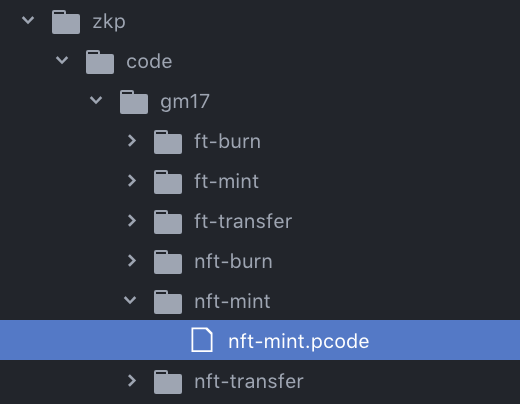
\includegraphics[width=0.7\textwidth]{files-before-setup.png}
	\end{minipage}
	\quad
	\begin{minipage}{0.3\textwidth}
		\centering
		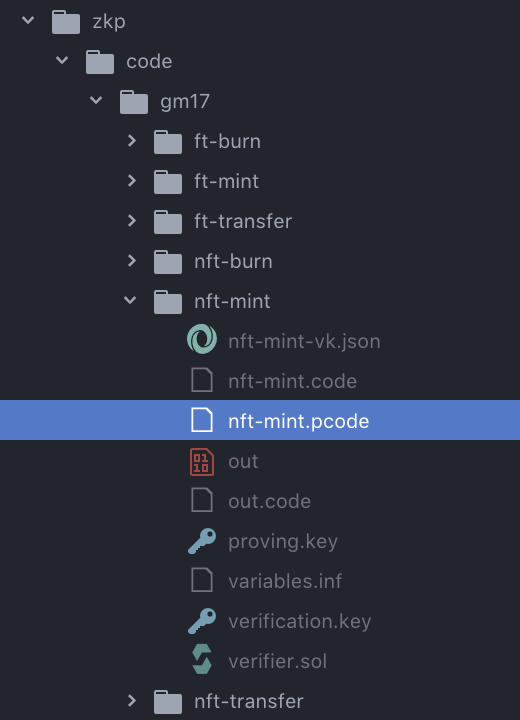
\includegraphics[width=0.7\textwidth]{files-after-setup.png}
	\end{minipage}
	\smallbreak
	\caption{Files in $\mathcal{T}$'s local repository before (left) and after (right) performing a trusted setup.}
	\label{pic:filesBeforeAfterSetup}
\end{figure}

The trusted setup abstracts the human-readable code of the ZoKrates DSL (files with a \texttt{.code} or \texttt{.pcode} extension) into a (proving key, verification key) pair.\\
\\
Suppose $\mathcal{T}$ is a `trusted benefactor' who intends to use Nightfall to set up the infrastructure which will allow anyone to transfer ownership of tokens under zero knowledge.
When $\mathcal{T}$ first clones the Nightfall repository, he only has human-readable computations written in \texttt{`.pcode'} syntax. Taking the \texttt{./zkp/code/gm17/nft-mint/} folder as an example, $\mathcal{T}$ will initially only have
\texttt{`nft-mint.pcode'}.  
The trusted setup will provide $\mathcal{T}$ with:
\texttt{`nft-mint-vk.json'}, \texttt{`nft-mint.code'},
\texttt{`out'}, \texttt{`out.code'}, \texttt{`proving.key'},
\texttt{`variables.inf'}, \texttt{`verification.key'},
\texttt{`verifier.sol'}.
This is shown in Figure~\ref{pic:filesBeforeAfterSetup} and a brief explanation of each of these files is provided in Table~\ref{table:trustedoutput}.

\begin{table}[h]
	\begin{center}
		\begin{tabular}[t]{L{0.2\textwidth}L{0.7\textwidth}}
			\toprule
			Trusted Setup Output & Explanation  \\ \midrule 
			\texttt{nft-mint-vk.json} & The verification key for an `nft-mint'. This will be stored on-chain, within the \hyperref[sec:smartContracts]{Verifier Registry}. Every time a user submits a (proof, public inputs) pair to the \hyperref[sec:smartContracts]{Shield contract}, this pair is verified with respect to the verification key within the \hyperref[sec:smartContracts]{Verifier contract}.
			\\
			\texttt{nft-mint.code} & Human-readable computation for an `nft-mint', written in the DSL of ZoKrates.
			\\
			\texttt{nft-mint.pcode} & An abbreviation of the \texttt{.code} syntax, for easier writing.
			\\
			\texttt{out} & Ignore. \\
			\texttt{out.code} & Ignore 
			\\
			\texttt{proving.key} & Used to generate proofs. Every time a User generates a new proof, this file is used by ZoKrates. 
			\\
			\texttt{variables.inf} & Ignore 
			\\
			\texttt{verification.key} & A representation of the verification key. Nightfall uses the jsonified version of the verification key (\texttt{mint-nft-vk.json}) and submits it as a flattened array to the \hyperref[sec:smartContracts]{Verifier Registry}.
			\\
			\texttt{verifier.sol} & Ignore.  This is an example implementation of a verifier contract with the verification key hard-coded into it.  It is unused by Nightfall. \\ \bottomrule
		\end{tabular}
	\end{center}
\caption{The files output by the trusted setup.}
\label{table:trustedoutput}
\end{table}

\textbf{Remark:}
The proving keys are by far the largest files required by Users of Nightfall:
\begin{center}
\begin{tabular}{ll}
	nft-mint & 77 MB\\
	nft-transfer & 1.1 GB\\
	nft-burn & 1.0 GB\\
	ft-mint & 77 MB\\
	ft-transfer & 2.1 GB\\
	ft-burn & 1.0 GB\\
\end{tabular}
\end{center}

The file sizes shown here reflect the sizes of the files once extracted from a ZoKrates container and stored on a User's local machine. (As opposed to the proving key sizes displayed in Table~\ref{table:efficiency}, which are calculated at setup time). The `transfer' and `burn' proving keys are particularly large, because of how a User proves that their token commitment exists as a leaf of the on-chain Merkle Tree (see \hyperref[part:theProtocols]{The Protocols}). As a default size, the on-chain Merkle Tree is 33-deep, meaning $32$ sha256 hashes are performed to calculate the root of the Merkle Tree from the relevant leaf. Each sha256 hash requires around $25,000$ constraints. For a fungible transfer, $64$ sha256 hashes are performed ($2 \times 32$).

Once $\mathcal{T}$ has completed the trusted setup for each of the six computations, he is ready to create the rest of the Nightfall infrastructure.
We outline his steps in Figure~\ref{fig:trustedSetup}. The Smart Contracts being alluded to are discussed in more detail in the \hyperref[sec:smartContracts]{Smart Contracts} section.
\begin{figure}[ht]
	\begin{center}
		\begin{framed}
      \begin{tabular}{p{16cm}}	
        \textbf{Deploying the Nightfall Infrastructure} \\ \midrule
         \\
        \textbf{Trusted Benefactor steps}:
        \begin{enumerate}
				  \item Perform the `Trusted Setup' to produce the proving key and the verification key for each of the six computations.
				  \item Share the proving keys with the world (e.g. through an online sharing service). Do not share the proving keys on a blockchain; they're way too big!
				  \item Locate the Verifier Registry contract's address on the Ethereum mainnet. We intend there to only be one Verifier Registry on the mainnet for all zk-SNARK traffic; in much the same way as the ENS registers all .eth domain names. Note, however, that the default migration scripts of the Nightfall repository do deploy an instance of a Verifier Registry, for example's sake.
          \item Either:
          \begin{itemize}
            \item Locate a GM17 verifier contract address on the Ethereum mainnet; or
            \item Deploy an instance of the GM17 verifier contract to the Ethereum mainnet. And register this GM17 verifier contract with the Verifier Registry (see \texttt{./zkp/src/vk-controller.js} which does this in the Nightfall repository).
          \end{itemize}
          \item Choose which ERC-20 token you wish for your new infrastructure to `shield'.
          \item Deploy an instance of the \texttt{FTokenShield.sol} contract to the Ethereum mainnet; specifying the addresses of the chosen GM17 verifier contract and chosen the ERC-20 contract, in the \texttt{constructor} of \texttt{FTokenShield.sol}.
          \item Choose which ERC-721 token you wish for your new infrastructure to `shield'.
          \item Deploy an instance of the \texttt{NFTokenShield.sol} contract to the Ethereum mainnet; specifying the addresses of the chosen GM17 verifier contract and chosen the ERC-721 contract, in the \texttt{constructor} of \texttt{NFTokenShield.sol}.
          \item Store all six verification keys in the Verifier Registry. (See \texttt{./zkp/src/vk-controller.js} which does this in the Nightfall repository). You will receive six \texttt{`vkId'} values from the Verifier Registry in return. These are unique identifiers for the six verification keys.
          \item Share the six \texttt{`vkId'} values with the world; (e.g. through the same online sharing service as the proving keys). It must be clear to Users which vkId corresponds to which proving key. \texttt{./zkp/src/\hyperref[sec:zkp]{vkIds.json}} gives an example of how to store these.
          \item Share the Ethereum addresses of the FtokenShield.sol and NFTokenShield.sol contracts.
          
          \setcounter{ongoingEnumCounter}{\value{enumi}}
        \end{enumerate}
        \ \\
        \midrule \\
        \textbf{User steps}:
        \begin{enumerate}
          %resume counter
          \setcounter{enumi}{\value{ongoingEnumCounter}}
          \item Download each proving key and its corresponding vkId from $\mathcal{T}$'s online sharing portal.
          \item Generate a \texttt{(proof, inputs)} pair, as explained in \hyperref[part:theProtocols]{The Protocols}.
          \item Submit the \texttt{(proof, inputs)} pair to the relevant Shield contract.
          
          E.g., using web3: \texttt{nfTokenShield.mint(proof, inputs, vkId)}
          \item Store relevant data in local database.
          \setcounter{ongoingEnumCounter}{0}
        \end{enumerate}
			\end{tabular}
		\end{framed}
	\end{center}
\caption{Deploying the Nightfall Infrastructure}
\label{fig:trustedSetup}
\end{figure}


\subsection*{Notes for a User}
Ordinary Users of a Nightfall infrastructure do not need to (and should not!) perform a trusted setup themselves. Only the original creator of the Shield contracts needs to.
The trusted setup involves a source of randomness and the (proving key, verification key) pair for a given computation will change each time the trusted setup is performed.
Therefore, if a User wishes to generate 'proofs' (zk-SNARKs) to be verified against a verification key which has been stored on the Ethereum mainnet, they should use the exact proving key and vkId which was generated by the trusted setup and shared with everyone.

To explain further, note that for each verification key stored on-chain, there is a corresponding and unique proving key which was generated at the same time, from the same randomness. It is this proving key which Users must use to generate proofs.
Using any other key the User's proofs will not verify against the verification key which has been stored on-chain.
If a User wishes to generate a proof against an existing, already-deployed verification key, they will need to request the corresponding proving key from the creator of the verification key.

\begin{figure}[H]
  \begin{center}
    \begin{mdframed}[backgroundcolor=verylightred]
      \noindent
      SECURITY WARNINGS 
        \begin{itemize}
          \item[--] Performing the initial 'trusted setup' of a computation -- to convert a \texttt{.code} file into a (proving key, verification key) pair -- requires the generation of some random numbers.\\
          \\
          Once the (proving key, verification key) pair has been generated from the \texttt{.code} file, these random numbers MUST be destroyed. These random numbers MUST never be stored by the party who performed the trusted setup, or that party would be able to generate false proofs which verify as \texttt{true}. These random numbers are often referred to as `toxic waste'.\\
          \\
          Nightfall leverages ZoKrates to perform the trusted setup, and relies on the proper management of the toxic waste by ZoKrates.\\
          \\
          A criticism of zk-SNARKs is that future users of a (proving key, verification key) pair, will have to trust that the party who performed the trusted setup (at the `beginning of time') did so properly and truthfully. 
        \end{itemize} 
    \end{mdframed} 
  \end{center}
  \caption{Security warning: Toxic Waste}
  \label{fig:trustedSetupWarning}
\end{figure}


\begin{center}
  \begin{mdframed}[backgroundcolor=verylightblue]
    Where to look?\\
    \\
    \begin{tabular}{lp{14cm}}
      \texttt{./zkp/code/gm17/nft-mint/nft-mint.pcode} & \texttt{.pcode} files with human-readable computations.\\
      \texttt{./zkp/code/gm17/nft-mint/nft-transfer.pcode} & \\
      \texttt{./zkp/code/gm17/nft-mint/nft-burn.pcode} & \\
      \texttt{./zkp/code/gm17/nft-mint/ft-mint.pcode} & \\
      \texttt{./zkp/code/gm17/nft-mint/ft-transfer.pcode} & \\
      \texttt{./zkp/code/gm17/nft-mint/ft-burn.pcode} & \\
      \texttt{./zkp/code/README-tools-trusted-setup.md} & README for automating the trusted setup.\\
      \texttt{./zkp/code/README-manual-trusted-setup.md} & README for manually performing the trusted setup.\\
      \url{https://github.com/Zokrates/ZoKrates} & ZoKrates source code\\
      \url{https://zokrates.github.io} & ZoKrates documentation\\
      \texttt{./zkp/code/README-tools-code-preprop.md} & explanation of \texttt{.pcode} syntax\\
      \url{https://github.com/EYBlockchain/zokrates-preprocessor} & how to manually transpile from \texttt{.pcode} to \texttt{.code}\\ 
      \texttt{./zkp/code/README-manual-trusted-setup.md} & how to manually do the trusted setup
    \end{tabular}
  \end{mdframed}
\end{center}

\newpage
\section{Smart Contracts}
\label{sec:smartContracts}
\secttoc

In this section we give further details of all the Solidity contracts, libraries and interfaces in the Nightfall repository.
Some of these contracts are pre-existing and some are new.
The important new contracts are:
\begin{itemize}
  \item Shield contract - stores `token commitments' which represent ownership of underlying ERC-20 or ERC-721 tokens, and facilitates the minting, transferring and burning of these token commitments.
  \item Verifier Contract - uses elliptic curve pairing functions to verify a zk-SNARK.
  \item Verifier Registry Contract - a registry of Verifier Contracts, Verification Keys, and Proof submissions. For simplicity, we ignore this layer from our explanations in this paper; although it is utilised in the Nightfall repository.
\end{itemize}

Here, we give further details of all Solidity contracts, libraries and interfaces in the Nightfall repository:\\
\\
\subsection{Pre-Existing Contracts}

\subsubsection{\texttt{ERC-721}}
The structuring of the ERC-721 contracts is aligned with the \url{https://0xcert.org} implementation.
These are designed for the transfer of non-fungible assets and include the following files:
\begin{center}
	\begin{tabular}{ll}
		\texttt{ERC721Interface.sol} & \\
		\texttt{ERC721TokenReceiver.sol} & \\
		\texttt{ERC721Metadata.sol} & \\
		\texttt{NFTokenMetadata.sol} & An example metadata implementation, to accompany \texttt{NFToken.sol} \\
		\texttt{NFToken.sol} & An example ERC-721 implementation.
	\end{tabular}
\end{center}
An overview of the ERC-721 contracts is given in Figure~\ref{pic:nftSmartContract}

\begin{figure}[H]
	\begin{center}
		\begin{mdframed}[backgroundcolor=black,userdefinedwidth=\textwidth,align=center]
			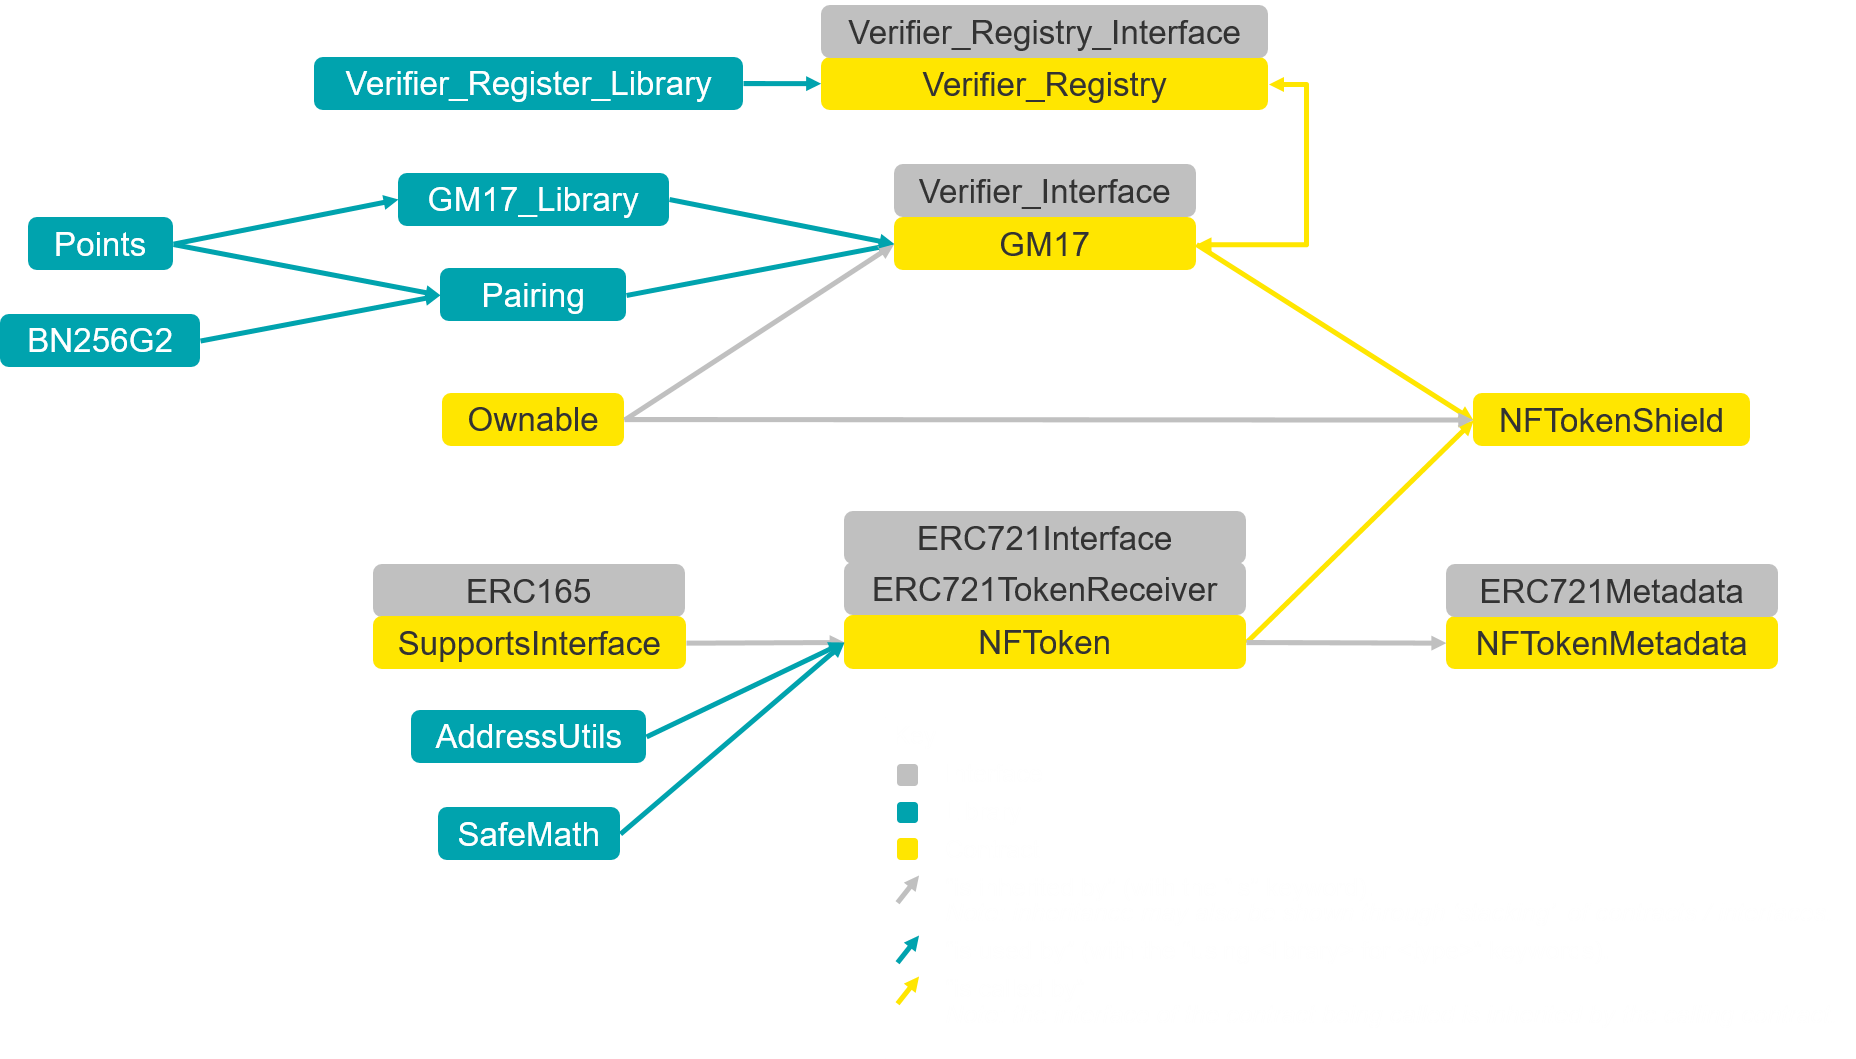
\includegraphics[width=\textwidth]{images/nft-contracts.png}
		\end{mdframed}
	\end{center}
	\caption{ERC-721 contract structure.}
	\label{pic:nftSmartContract}
\end{figure}

\subsubsection{\texttt{ERC-20}}
The structuring of the ERC-20 contracts is aligned with the \url{https://openzeppelin.org} implementation.
These are designed for the transfer of fungible assets and include the following files: 
\begin{center}
	\begin{tabular}{ll}
		\texttt{ERC20Interface.sol} & \\
		\texttt{FToken.sol} & An example ERC-20 implementation. \\
	\end{tabular}
\end{center}
An overview of the ERC-20 contracts is given in Figure~\ref{pic:ftSmartContract}

\begin{figure}[H]
	\begin{center}
		\begin{mdframed}[backgroundcolor=black,userdefinedwidth=\textwidth,align=center]
		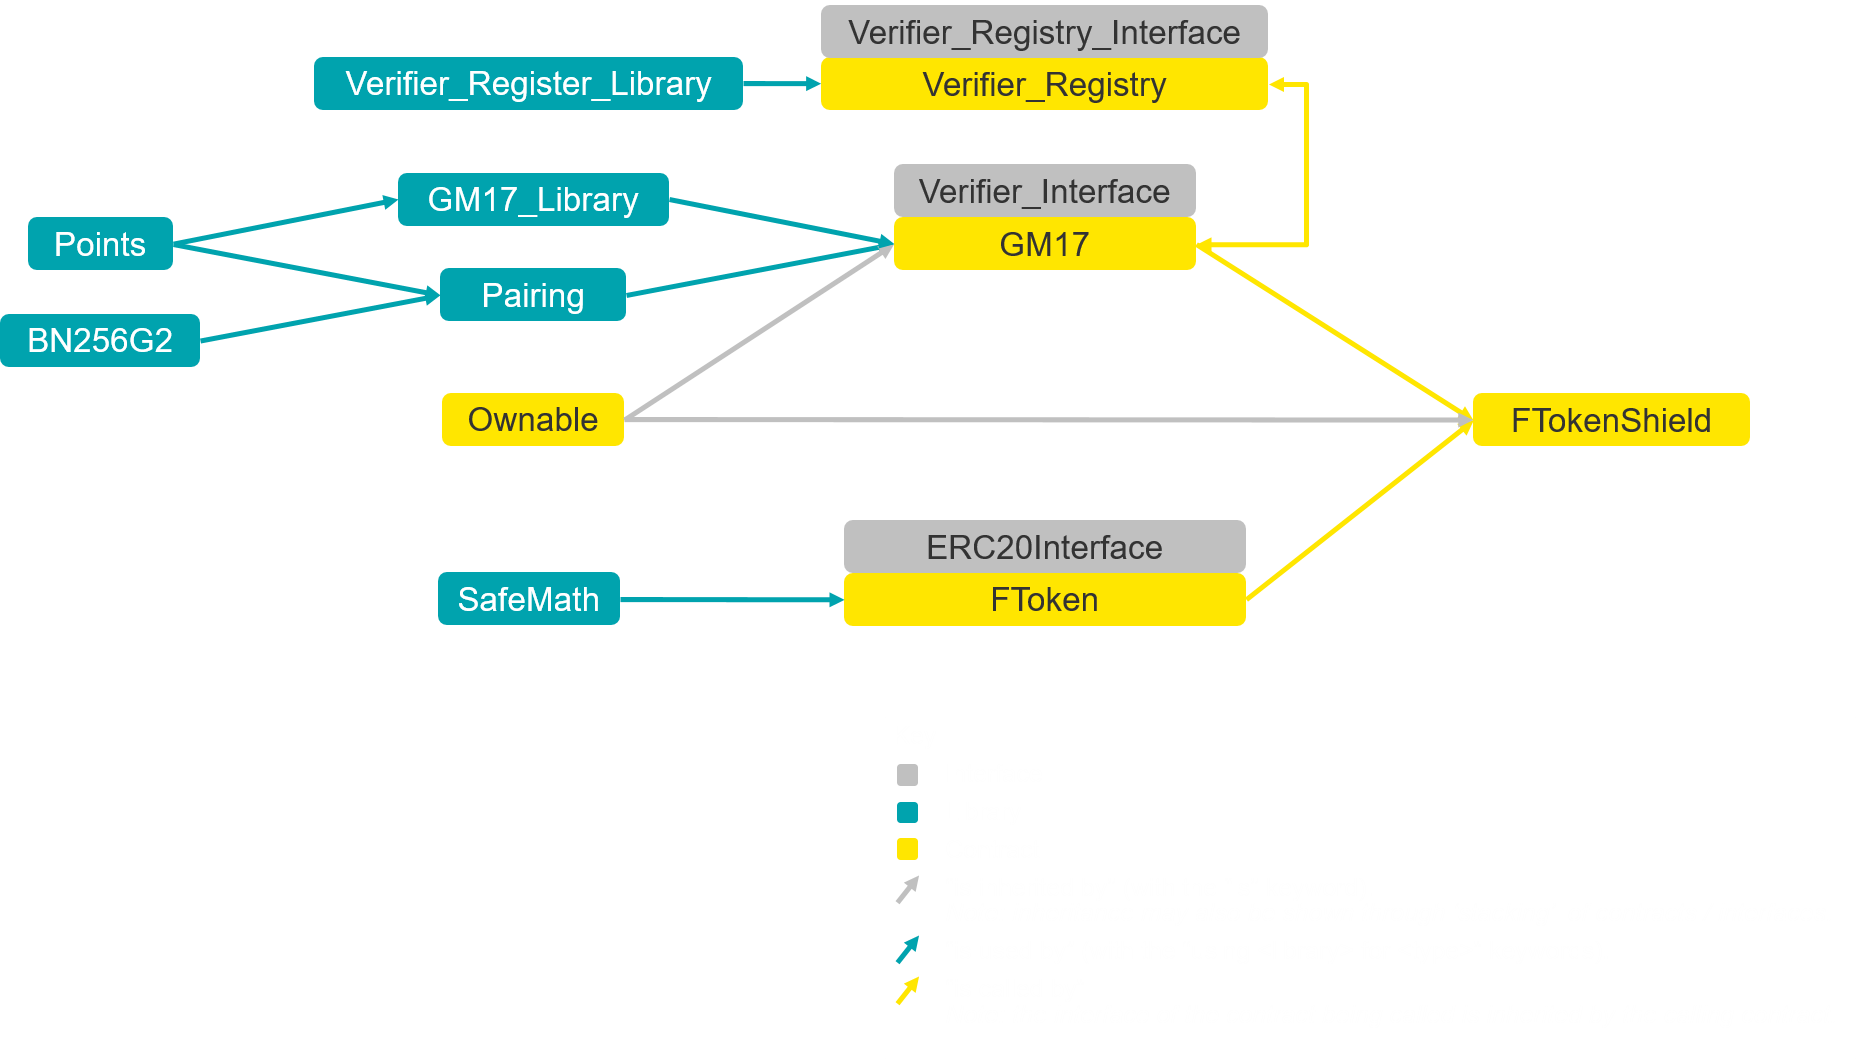
\includegraphics[width=\textwidth]{images/ft-contracts.png}
		\end{mdframed}
	\end{center}
	\caption{ERC-20 contract structure.}
	\label{pic:ftSmartContract}
\end{figure}

\subsubsection{\texttt{ERC-165}}
The structuring of the ERC-165 contracts is aligned with the \url{https://0xcert.org} implementation.
\begin{center}
	\begin{tabular}{ll}
		\texttt{ERC165Interface.sol} & \\
		\texttt{SupportsInterface.sol} &  \\
	\end{tabular}
\end{center}

\subsubsection{\texttt{Utility contracts}}
\begin{center}
	\begin{tabular}{ll}
		\texttt{AddressUtils.sol} & See \url{https://ethereum.stackexchange.com/a/14016/36603} for more details about how this works. \\
		\texttt{SafeMath.sol} & For safe mathematical operations.  \\
	\end{tabular}
\end{center}

\subsection{Shield contracts}
\subsubsection{\texttt{NFTokenShield.sol}}
Facilitates private transfers of Non-Fungible Tokens.

Constructor: At deployment, specify one Verifier contract (see below) and one ERC-721 contract. NFTokenShield will then be able to hold tokens of the ERC-721 contract in escrow, whilst the private counterparts of these tokens are transferred. Future contributions to Nightfall will produce an NFTokenShield contract which can handle multiple ERC-721 contracts at once.

Stores token commitments, which represent ownership of a token of the specified ERC-721 contract.

Calls upon the Verifier contract to verify zk-SNARKs for it.

A high-level diagram of the `shielding' process is shown in Figure~\ref{pic:nftShield}.

\begin{figure}[H]
	\begin{center}
		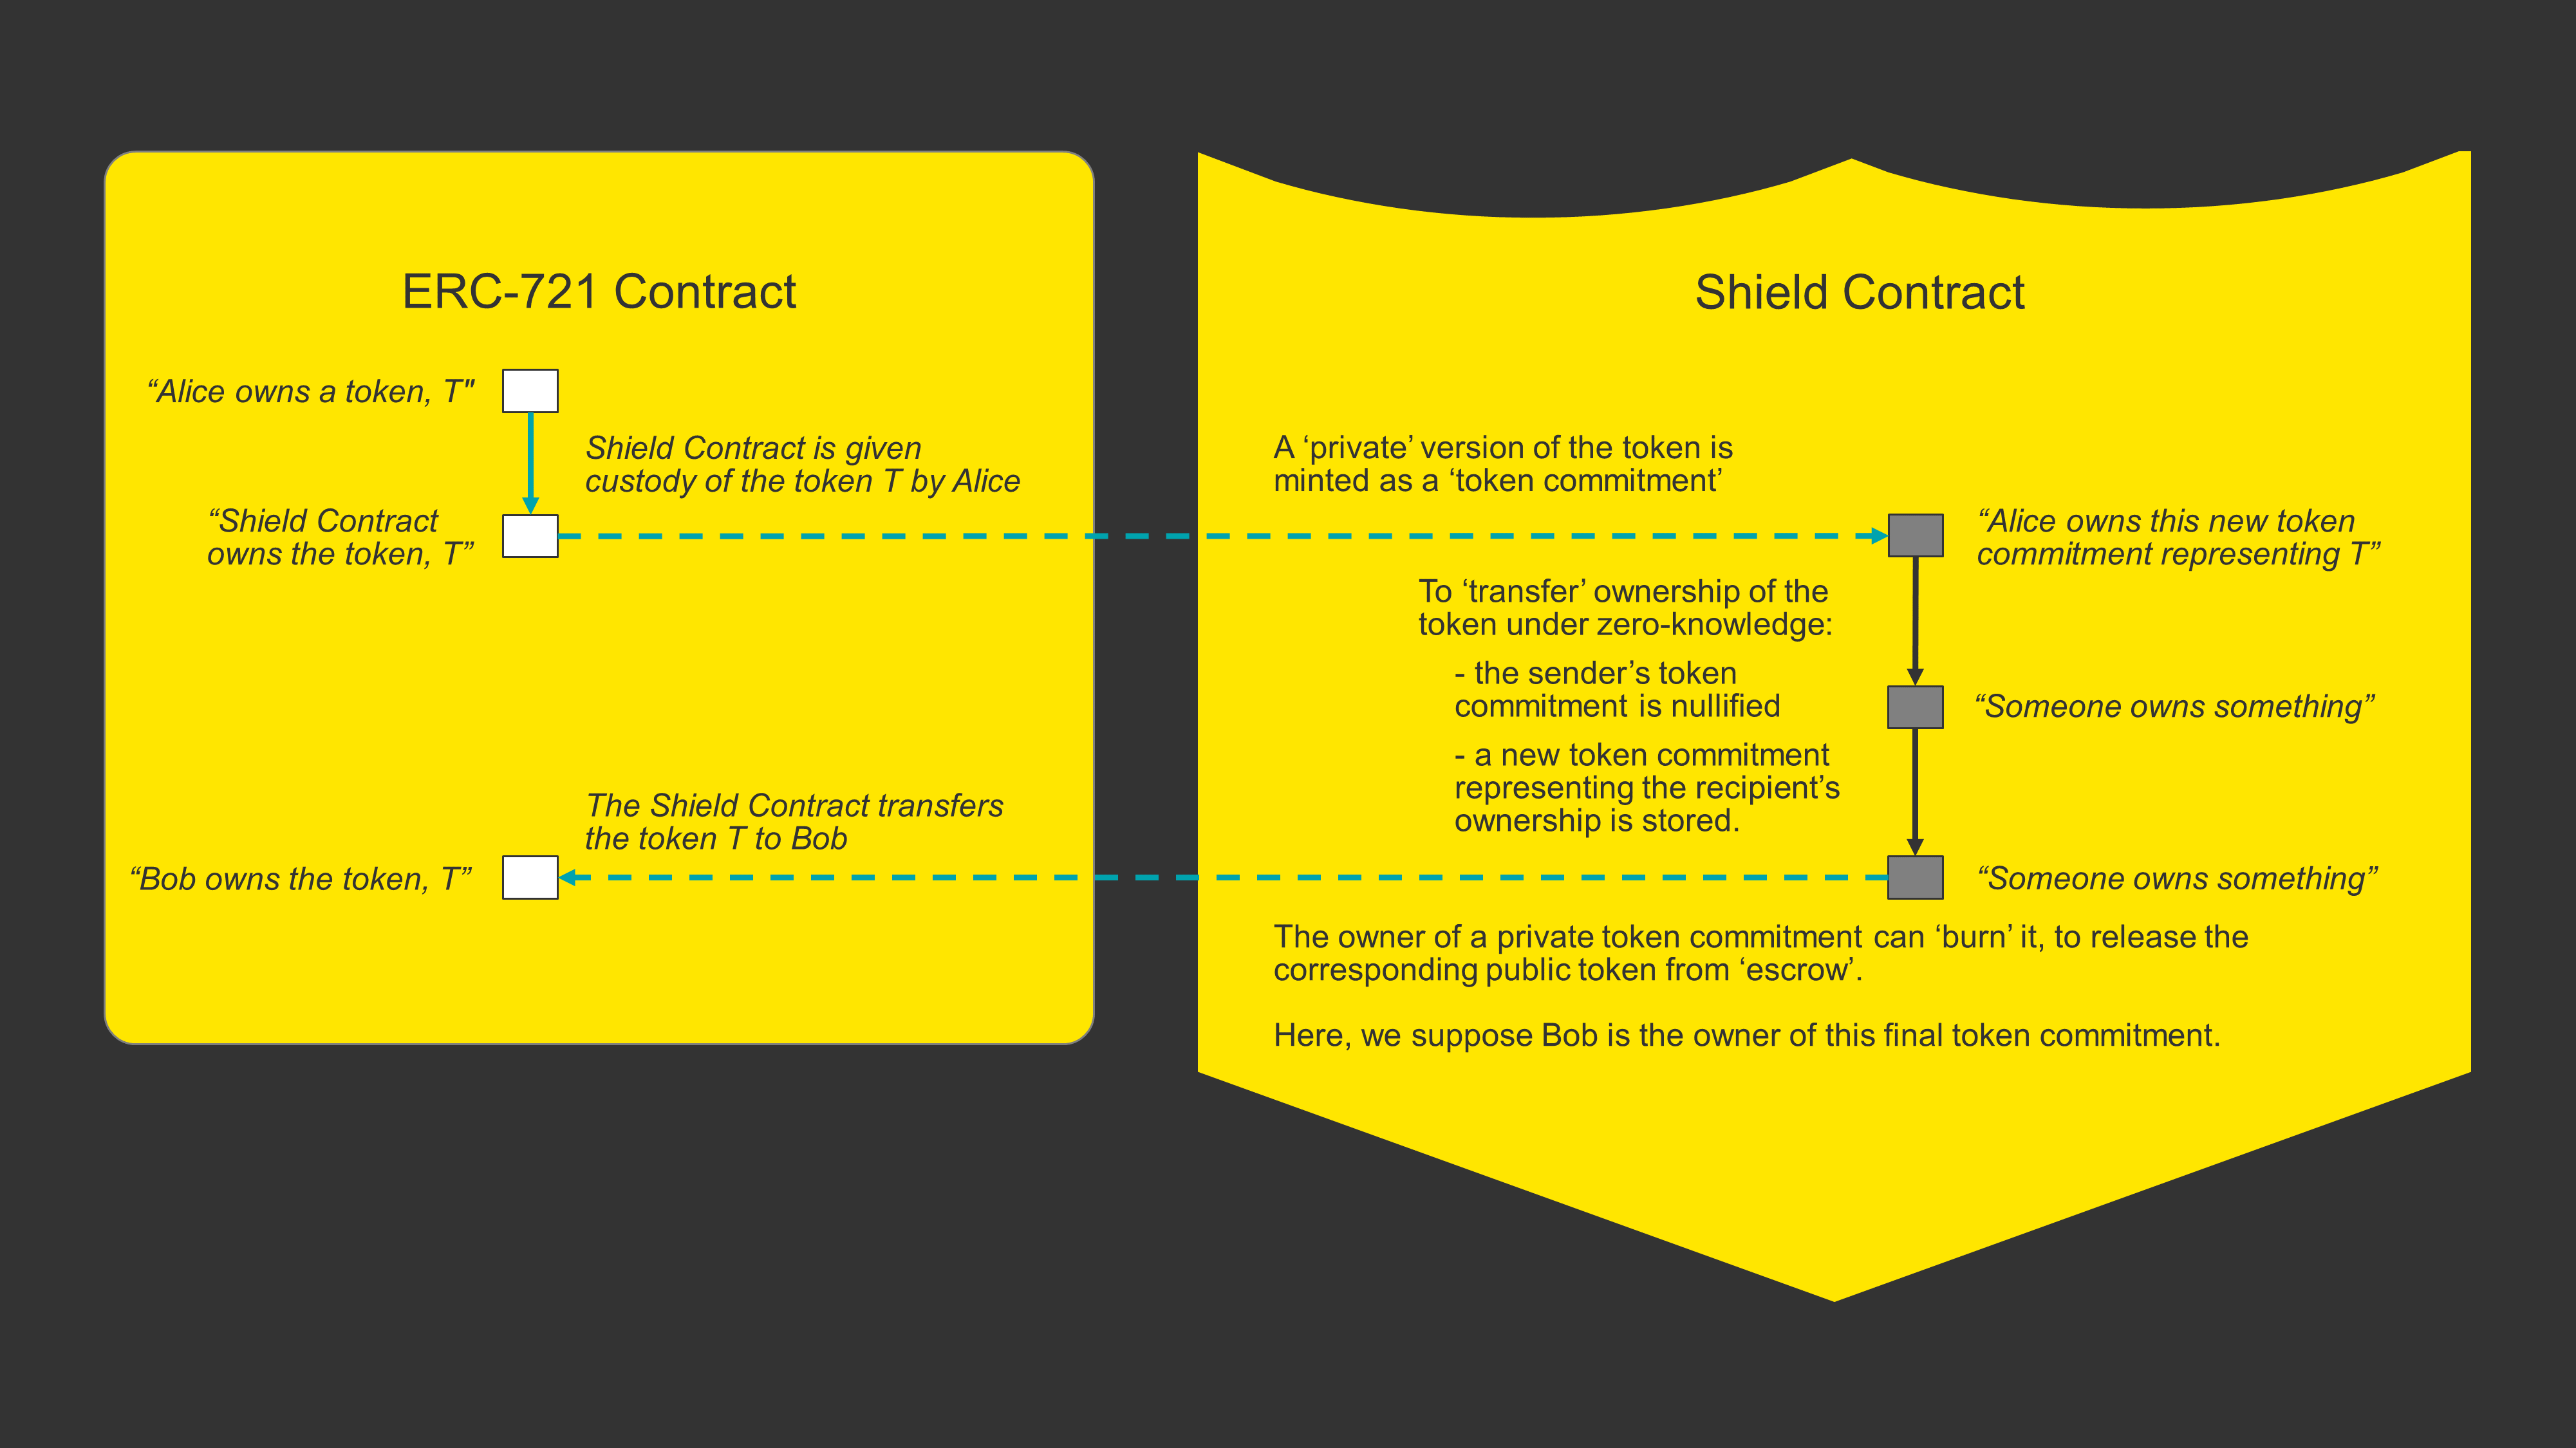
\includegraphics[width=\textwidth]{images/erc721Shielding.png}
	\end{center}
	\caption{High-level diagram of `shielding' an ERC-721 token.}
	\label{pic:nftShield}
\end{figure}

\subsubsection{\texttt{FTokenShield.sol}}
Facilitates private transfers of Fungible Tokens.

Constructor: At deployment, specify one Verifier contract (see below) and one ERC-20 contract. FTokenShield will then be able to hold tokens of the ERC-20 contract in escrow, whilst the private counterparts of these tokens are transferred. Future contributions to Nightfall will produce an FTokenShield contract which can handle multiple ERC-20 contracts at once.

Stores token commitments, which represent ownership of a particular amount of currency, as denominated in the specified ERC-20 contract.

Calls upon the Verifier contract to verify zk-SNARKs for it.

A high-level diagram of the `shielding' process is shown in Figure~\ref{pic:ftShield}.

\begin{figure}[H]
	\begin{center}
		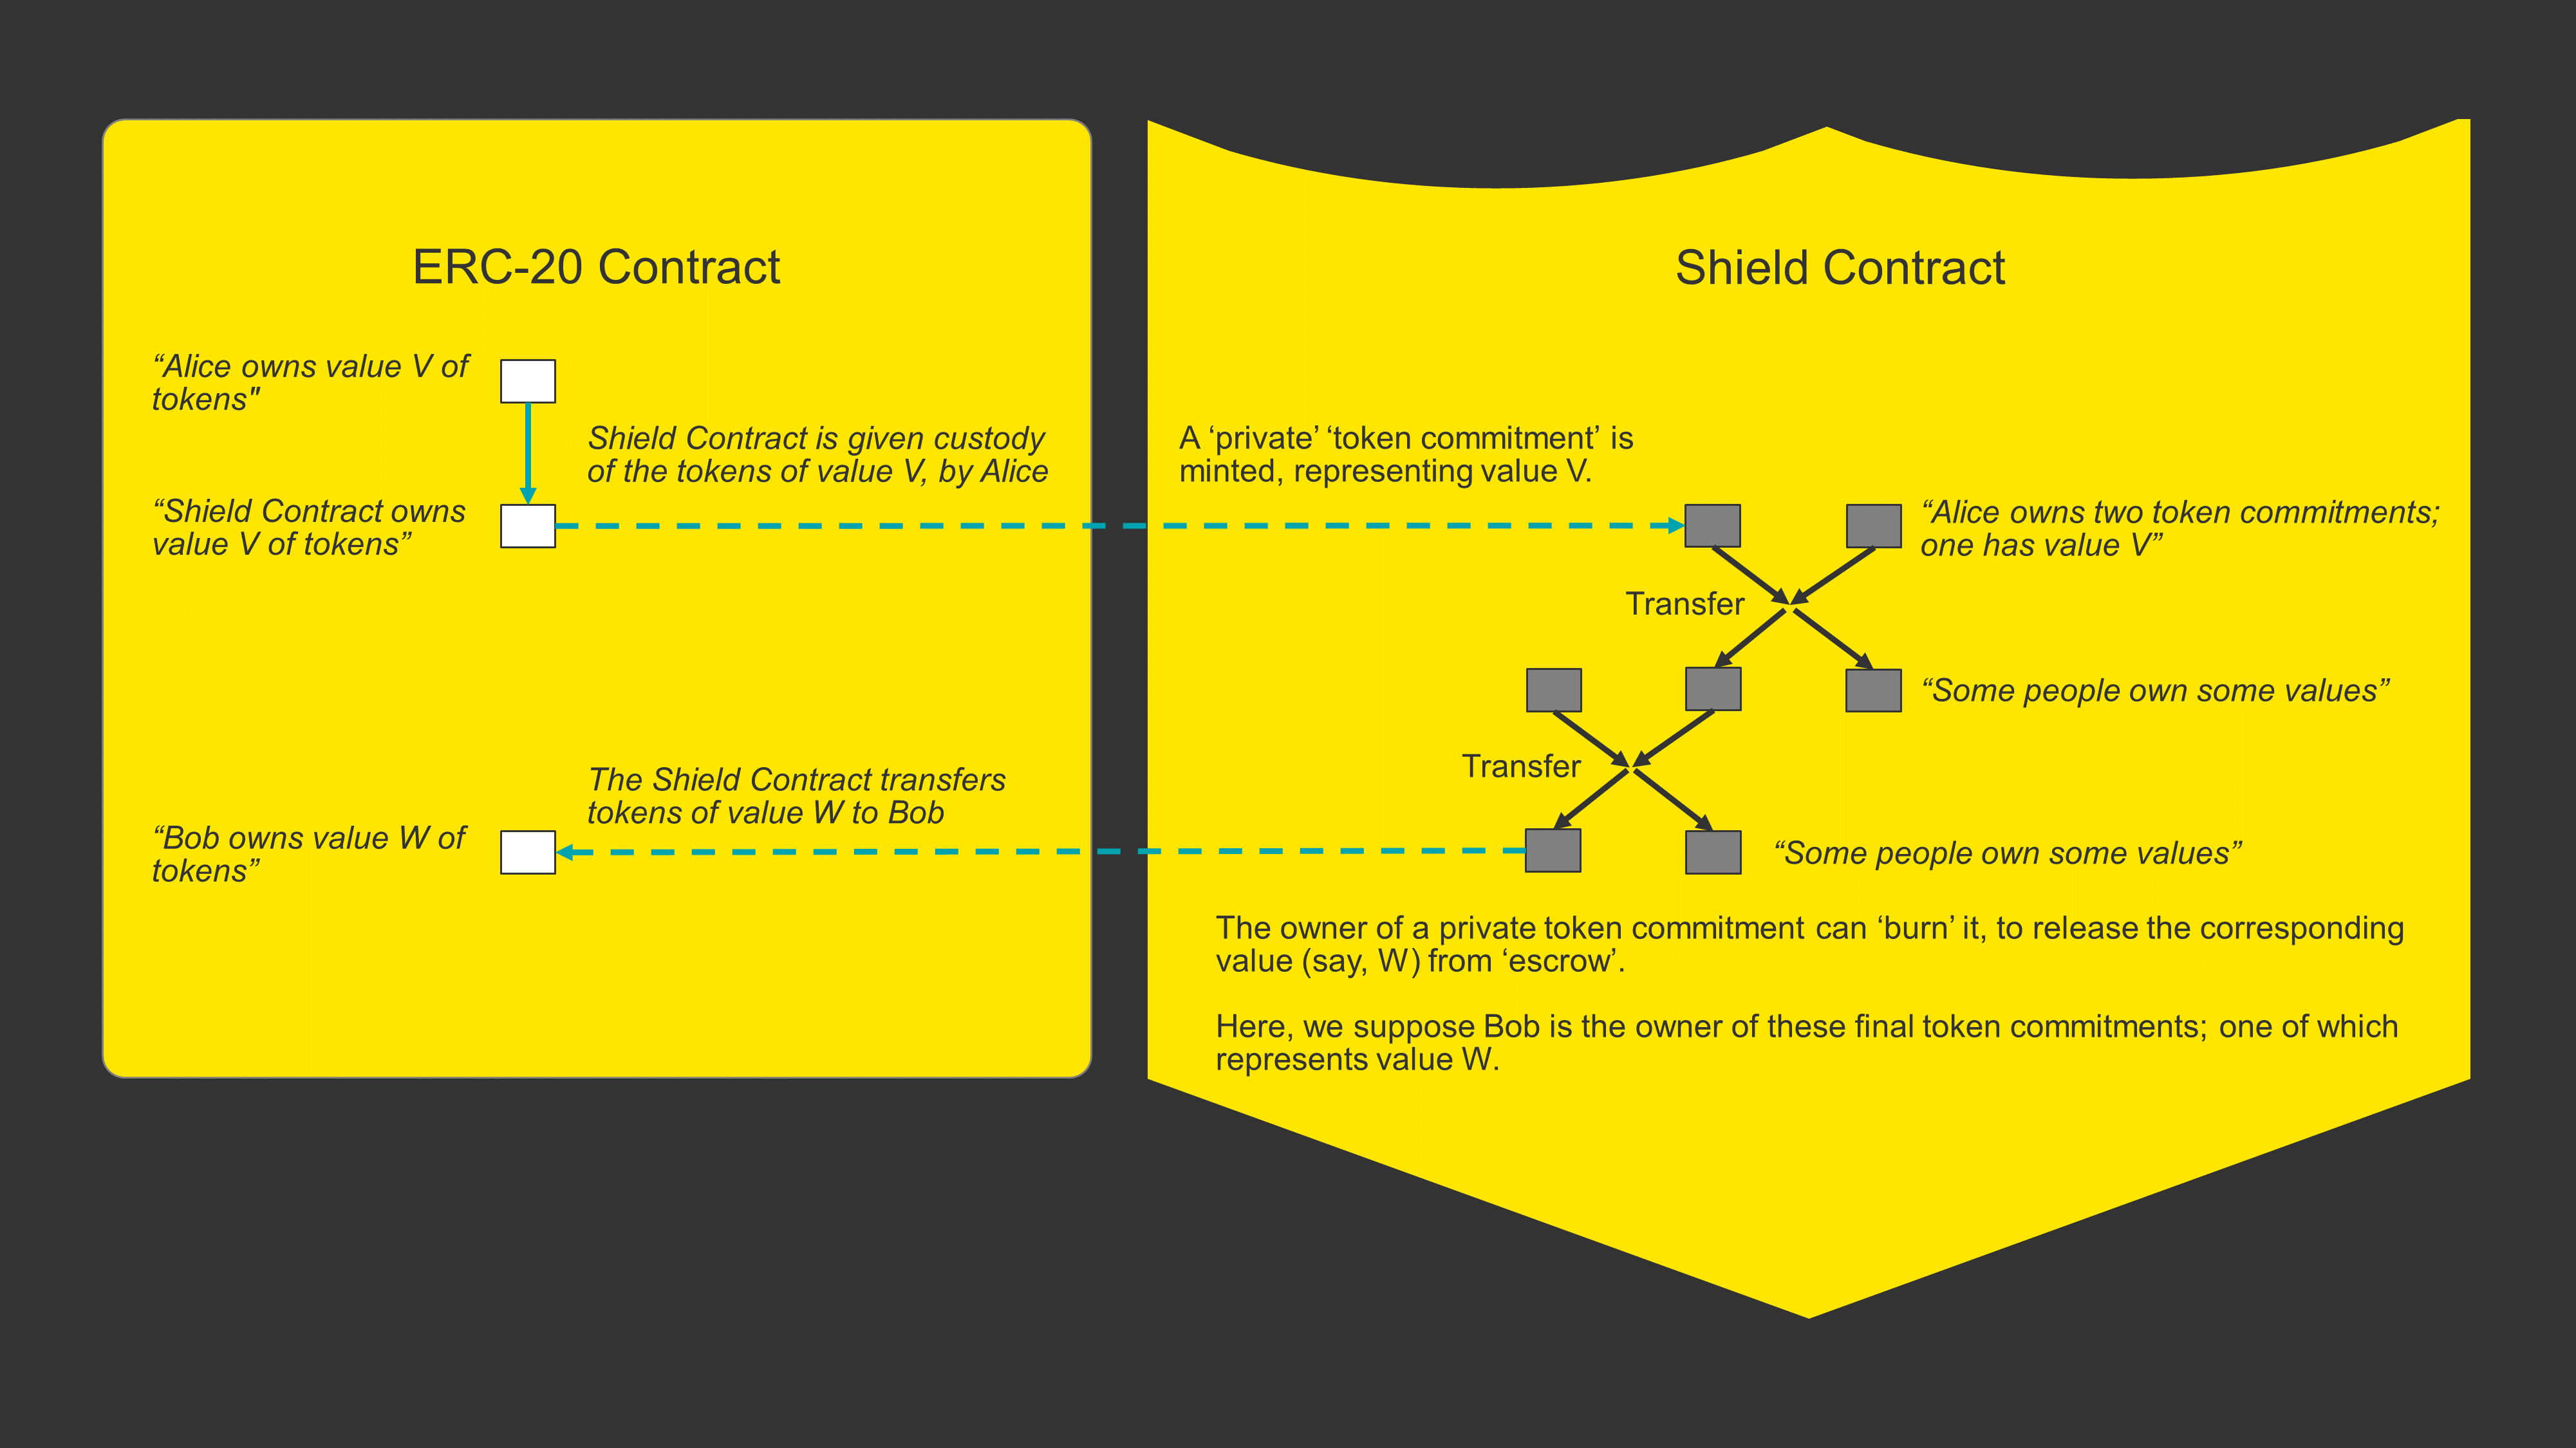
\includegraphics[width=\textwidth]{images/erc20Shielding.png}
	\end{center}
	\caption{High-level diagram of `shielding' an ERC-20 token.}
	\label{pic:ftShield}
\end{figure}

\subsection{Verifier contracts}
The sole purpose of a verifier contract is to verify zk-SNARKs which are passed to it. It returns \texttt{true} if the (proof, public inputs) pair verifies. Otherwise, it returns \texttt{false}.

\subsubsection{\texttt{GM17.sol}}
An implementation of the draft EIP-1922 zk-SNARK Verifier Standard. 

\subsubsection{\texttt{Points.sol}}
Library. Defines how Elliptic Curve coordinates $(x, y)$ are structured.

\subsubsection{\texttt{GM17Library.sol}}
Library. Defines the structures of both a Verification Key and a Proof under the GM17 protocol (using the elliptic curve points of \texttt{Points.sol}).

\subsubsection{\texttt{Pairing.sol}}
Library. Performs elliptic curve operations and elliptic curve pairing operations. Utilises the precompiled contracts of EIP-196 and EIP-197.

\subsection{Verifier Registry contracts}
The Verifier Registry is intended to be a single contract to register all zk-SNARK traffic on the Ethereum mainnet. It facilitates:
\begin{itemize}
  \item[--] Registration of Verifier contracts 
  \item[--] Storage of all Verification Keys
  \item[--] Proof submissions 
  \item[--] Other zk-SNARK use-cases beyond Nightfall 
\end{itemize}

Note: although the intention is for there to be just one Verifier Registry on the Ethereum mainnet, the default migration script in the Nightfall repository deploys an implementation of the Verifier Registry along with all other contracts -- for the sake of example.

\subsubsection{\texttt{Verifier\_Registry\_Interface.sol}}
The draft EIP-1923 interface for a Verifier Registry.

\subsubsection{\texttt{Verifier\_Registry.sol}}
An implementation of the Verifier\_Registry\_Interface.

\subsubsection{\texttt{Verifier\_Register\_Interface.sol}}
Library. Defines the structures of the register, which store entries to the Verifier\_Registry.

\subsection{Deployment of Contracts}
\label{sec:deploymentOfContracts}
See \hyperref[fig:trustedSetup]{Trusted Setup} for an explanation of deployment steps, and how contract deployment is intertwined with the zk-SNARK trusted setup.

\begin{center}
	\begin{mdframed}[backgroundcolor=verylightblue]
		Where to look?\\
		\\
		\begin{tabular}{lp{14cm}}
			\texttt{./zkp/contracts/} & Contracts in Nightfall\\
			\texttt{./zkp/migrations/} & Default deployment ordering of contracts in Nightfall\\
			\url{https://eips.ethereum.org/EIPS/eip-165} & EIP-165\\
			\url{https://eips.ethereum.org/EIPS/eip-20} & EIP-20\\
			\url{https://eips.ethereum.org/EIPS/eip-721} & EIP-721\\
			\url{https://eips.ethereum.org/EIPS/eip-196} & EIP-196\\
			\url{https://eips.ethereum.org/EIPS/eip-197} & EIP-197\\
			\url{https://eips.ethereum.org/EIPS/eip-1922} & EIP-1922\\
			\url{https://eips.ethereum.org/EIPS/eip-1923} & EIP-1923
		\end{tabular}
	\end{mdframed}
\end{center}




%Don't include figure until we get more. It looks out of place.
% \begin{figure}[H]
%   \centering
%   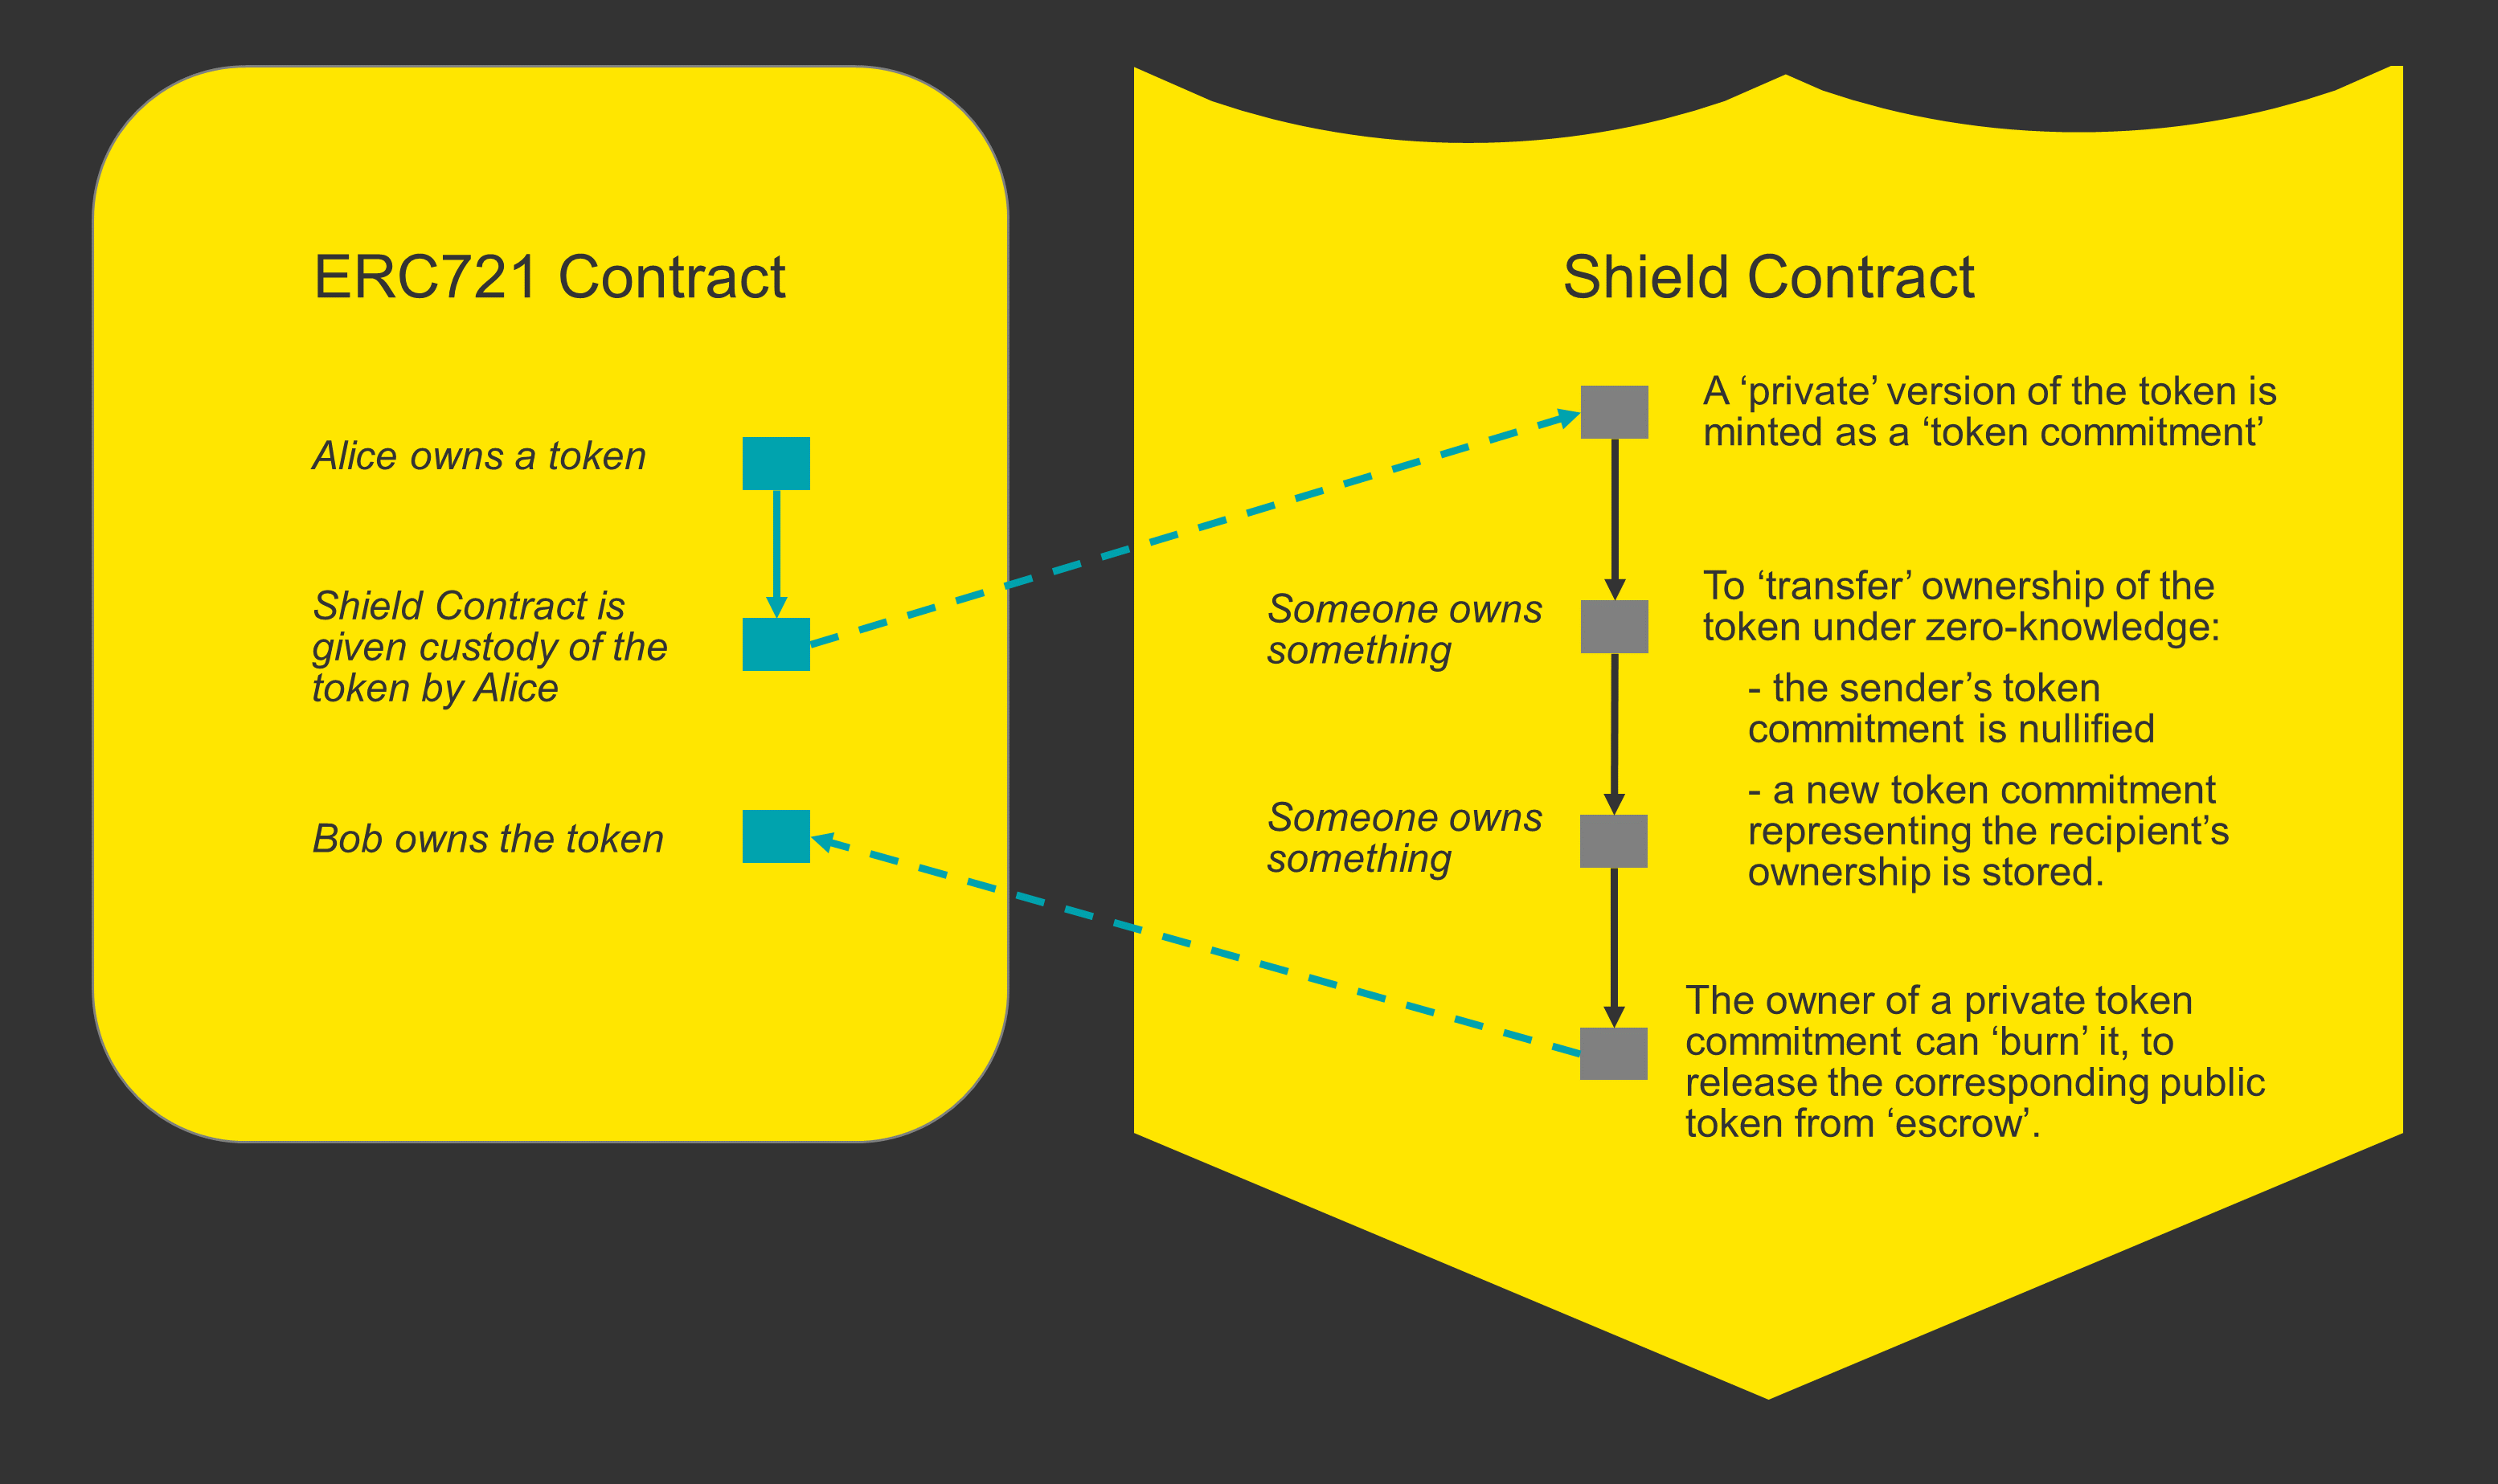
\includegraphics[scale=0.65]{smart-contracts}
%   \caption{The on-chain relationship between a `public' ERC-721 token and the `private' token commitments which represent it within the Shield Contract.}
%   \label{pic:Shield1}
% \end{figure}

\newpage
\section{Microservices}
\label{sec:microservices}
\secttoc

\subsection{zkp}
\label{sec:zkp}

\subsubsection{\texttt{f-token-controller.js}}
\label{sec:f-token-controller}
Functions to orchestrate mint, transfer, and burn of fungible token commitments.
\begin{itemize}
  \item[--] Receives public inputs from the front end;
  \item[--] Calculates the public inputs of each zk-SNARK;
  \item[--] Calls \texttt{zokrates.js} -- the ZoKrates JS wrapper -- to compute a witness and to generate a proof.
  \item[--] Calls \texttt{f-token-zkp.js} -- a web3 transactions module which sends transactions to relevant smart contracts.
\end{itemize} 

\subsubsection{\texttt{f-token-zkp.js}}
\label{sec:f-token-zkp}
Functions to send transactions (relating to fungible commitments) to the smart contracts. Using web3, this js module sends transactions to \texttt{FTokenshield}, \texttt{GM17}, and \texttt{Verifier\_Registry}.

\subsubsection{\texttt{nf-token-controller.js}}
\label{sec:nf-token-controller}
Functions to orchestrate mint, transfer, and burn of non-fungible token commitments.
\begin{itemize}
  \item[--] Receives public inputs from the front end;
  \item[--] Calculates the public inputs of each zk-SNARK;
  \item[--] Calls \texttt{zokrates.js} -- the ZoKrates JS wrapper -- to compute a witness and to generate a proof.
  \item[--] Calls \texttt{nf-token-zkp.js} -- a web3 transactions module which sends transactions to the \texttt{NFTokenShield} contract.
\end{itemize}

\subsubsection{\texttt{nf-token-zkp.js}}
\label{sec:nf-token-zkp}
Functions to send transactions (relating to non-fungible commitments) to the smart contracts. Using web3, this js module sends transactions to \texttt{NFTokenshield}, \texttt{GM17}, and \texttt{Verifier\_Registry}.

\subsubsection{\texttt{zokrates.js}}
JS wrapper functions for executing ZoKrates commands within a ZoKrates container. See \hyperref[sec:zokrates]{ZoKrates}.

\subsubsection{\texttt{vk-controller.js}}
Functions to send verification keys to the \texttt{Verifier\_Registry} contract. See \hyperref[sec:trustedSetup]{Trusted Setup} for context.

\subsubsection{\texttt{vkIds.json}}
JSON file which stores the vkId's for each of the six zk-SNARK computations (fungible mint, transfer and burn; and non-fungible mint, transfer and burn).\\
At the time the verification keys are deployed to the \texttt{Verifier\_Registry}, it returns a unique vkId for each verification key. \texttt{vkIds.json} also stores the Ethereum address of the smart contract to which the verification keys were submitted. See \hyperref[sec:trustedSetup]{Trusted Setup} for context.

\subsubsection{\texttt{stats.json}}
JSON file which stores -- for each of the six zk-SNARK computations -- the time it took to `compute-witness' and `generate-proof' within the ZoKrates container on the User's computer. These time statistics serve as `ETA' estimates for the next time the User generates a proof (and the command line displays a progress bar accordingly).

\begin{center}
  \begin{mdframed}[backgroundcolor=verylightblue]
    Where to look?\\
    \\
    \begin{tabular}{lp{14cm}}
      \texttt{./zkp/} & The zkp microservice\\
    \end{tabular}
  \end{mdframed}
\end{center}


\subsection{offchain}
\label{sec:offchain}

\subsubsection{whisper}
\label{sec:whisper}

\begin{center}
  \begin{mdframed}[backgroundcolor=verylightblue]
    Where to look?\\
    \\
    \begin{tabular}{lp{14cm}}
      \url{https://github.com/ethereum/wiki/wiki/Whisper} & Whisper GitHub.\\
      \url{https://web3js.readthedocs.io/en/1.0/web3-shh.html} & web3 for whisper\\
      \texttt{./offchain/whisper-controller-stub.js} & A whisper js wrapper for Ganache\\
      \texttt{./offchain/whisper-controller.js} & A whisper js wrapper for Geth\\
      \texttt{./offchain/listners.js} & \makecell[lt]{Listens for messages on behalf of the user.\\
      Decrypts relevant messages.\\
      Forwards the data to the relevant microservice to\\
      take action.\\
      E.g. to store new data in the database.}\\
    \end{tabular}
  \end{mdframed}
\end{center}

\begin{figure}[h]
  \begin{center}
    \begin{mdframed}[backgroundcolor=verylightred]
      \noindent
      LIMITATION\\
      \\
      The \texttt{whisper-controller.js} and The \texttt{whisper-controller-stub.js} only listen for Whisper events (via the \texttt{`subscribe'} methods) \textbf{when the user is logged into the Application}.\\
      \\
      If a user logs out, they will miss any incoming Whisper messages. E.g. Bob might not receive notification from Alice that he has been sent a commitment, and will not receive details of the preimage of the commitment, nor the location of the commitment within the on-chain Merkle Tree.\\
      \\
      This can be solved with future contributions to the Nightfall repository. Indeed, web3.shh includes the functionality to retrieve past messages already.
    \end{mdframed}
  \end{center}
  \caption{Limitation: Nightfall does not currently receive Whisper messages if the User is not logged in.}
  %\label{fig:nfMintWarning}
\end{figure}

\subsubsection{pkd}
\label{sec:pkd}

Nightfall uses a PKD (Public Key Directory) contract to allow users to lookup both ZKP public keys and Whisper public keys. See \hyperref[part:theProtocols]{The Protocols} for a disambiguation of the different public keys used in Nightfall. The public keys of a user can be retrieved with knowledge of their Ethereum Address.\\
\\
The PKD also serves as a simple Name Service; users can register a unique name with the PKD. With this, the public keys of a user can also be retrieved with knowledge of their unique name.\\
\\
An example usage of the PKD is:\\
If Bob wishes to ask Alice to send him an ERC-721 commitment under zero-knowledge: Bob can query Alice's Whisper public key from the PKD, and Alice can then query Bob's ZKP public key from the PKD.


\subsection{accounts}
\label{sec:accounts}

The `accounts' microservice manages a User's Ethereum accounts. (We use the terms Ethereum `address' and Ethereum `account' interchangeably).\\
\\
For a user, Alice, her anonymity is preserved by using a new `throwaway' Ethereum address each time she transacts with the Shield contract.\\
\\
This microservice generates new Ethereum accounts, and keeps track of them for the application.\\
\\
\textit{``But how would Alice pay for the gas costs of sending such a transaction to the Shield contract?''}\\
\\
She would have to pay for the verification computation of her zk-SNARK, and for the persistent storage of the public inputs to her zk-SNARK. In order for Alice to fund a new Ethereum account completely anonymously, she would have to mine Ether. This might not be a viable solution for some; as mining rewards can be unpredictable and could be insufficient to cover the gas needed to transact using Nightfall.\\
\\
Alternatively, Alice could make each transaction through a delegated third-party, who would send the \texttt{`transfer'} transaction on Alice's behalf. The initial release of Nightfall does not include functionality to delegate transactions to others. Nevertheless, we know that in future updates we can solve the problem of hiding that ``Alice transferred something'' so that observers only see that ``someone transferred something''.

\begin{figure}[h]
  \begin{center}
    \begin{mdframed}[backgroundcolor=verylightred]
      \noindent
      PRIVACY WARNING\\
      \\
      The initial release of Nightfall does not give Alice full anonymity when she interacts with the Shield contract, unless she mines into her anonymous Ethereum accounts.\\
      \\
      Future updates will include the functionality to delegate transactions to others. This is a solved problem, which just needs to be implemented.
    \end{mdframed}
  \end{center}
  \caption{Privacy warning: A future update is required to Nightfall to allow user's to reliably and consistently transact with the Shield contract anonymously.}
  %\label{fig:nfMintWarning}
\end{figure}

\begin{center}
  \begin{mdframed}[backgroundcolor=verylightblue]
    Where to look?\\
    \\
    \begin{tabular}{lp{14cm}}
      \texttt{./accounts/} & The accounts microservice\\
    \end{tabular}
  \end{mdframed}
\end{center}

\subsection{database}
\label{sec:database}

Nightfall uses mongodb to store private data on a User's local machine.

\begin{figure}[h]
  \begin{center}
    \begin{mdframed}[backgroundcolor=verylightred]
      \noindent
      SECURITY WARNING\\
      \\
      Currently, the `secret keys' for spending token commitments are stored in a User's `User' db. This is not particularly secure, and moderations might need to be made when creating production-ready applications.
    \end{mdframed}
  \end{center}
  \caption{Security warning: Secret keys are currently stored in the User's db.}
  %\label{fig:nfMintWarning}
\end{figure}


\begin{center}
  \begin{mdframed}[backgroundcolor=verylightblue]
    Where to look?\\
    \\
    \begin{tabular}{lp{14cm}}
      \texttt{./database/src/models/} & All schemas.\\
    \end{tabular}
  \end{mdframed}
\end{center}



\subsection{ui}
\label{sec:ui}

See the dedicated README for instructions on how to use the UI.\\

\begin{figure}[H]
  \begin{center}
    \begin{mdframed}[backgroundcolor=verylightred]
      \noindent
      SECURITY WARNING\\
      \\
      Currently, random salt values (denoted $\sigma$ in this document) are generated within the UI microservice, or within the api-gateway microservice.\\
      \\
      Ensure you're comfortable with the level of randomness achieved by these random number generators.
    \end{mdframed}
  \end{center}
  \caption{Security warning: Ensure you're comfortable with any random number generation in the application}
  %\label{fig:nfMintWarning}
\end{figure}

\begin{center}
  \begin{mdframed}[backgroundcolor=verylightblue]
    Where to look?\\
    \\
    \begin{tabular}{lp{14cm}}
      \texttt{./ui-src/} & The UI microservice\\
      \texttt{UI.md} & A demonstration of the UI\\
    \end{tabular}
  \end{mdframed}
\end{center}




\newpage
\section{Finite Fields and Bit Lengths}
\label{sec:finiteFieldsAndBitLengths}

\noindent
For those who go through the Nightfall code, you might realise there are many number conversions being made in the zkp microservice. In particular, there are frequently conversions and restrictions to $216$-bit ($27$-byte) values in much of today's Nightfall code. These conversions are a consequence of working with zk-SNARKs.\\
\\
Like many cryptographic protocols, zk-SNARKs make use of representing numbers as points on an elliptic curve. In doing so, the results of our computations become quite difficult to `unravel' -- that is, given an output, it becomes computationally infeasible for someone to determine the inputs. However, it also restricts the mathematics we can do. This is a gross oversimplification of why elliptic curves are used, but let's talk about them.\\
\\
Currently on Ethereum, there is only one elliptic curve for which it is `cheap' (in terms of gas costs) to perform calculations (due to there being precompile contracts supporting calculations on this curve):
\begin{align*}
    E := y^2 = x^3 + 3
\end{align*}

This curve looks like this:
\begin{figure}[H]
	\begin{center}
		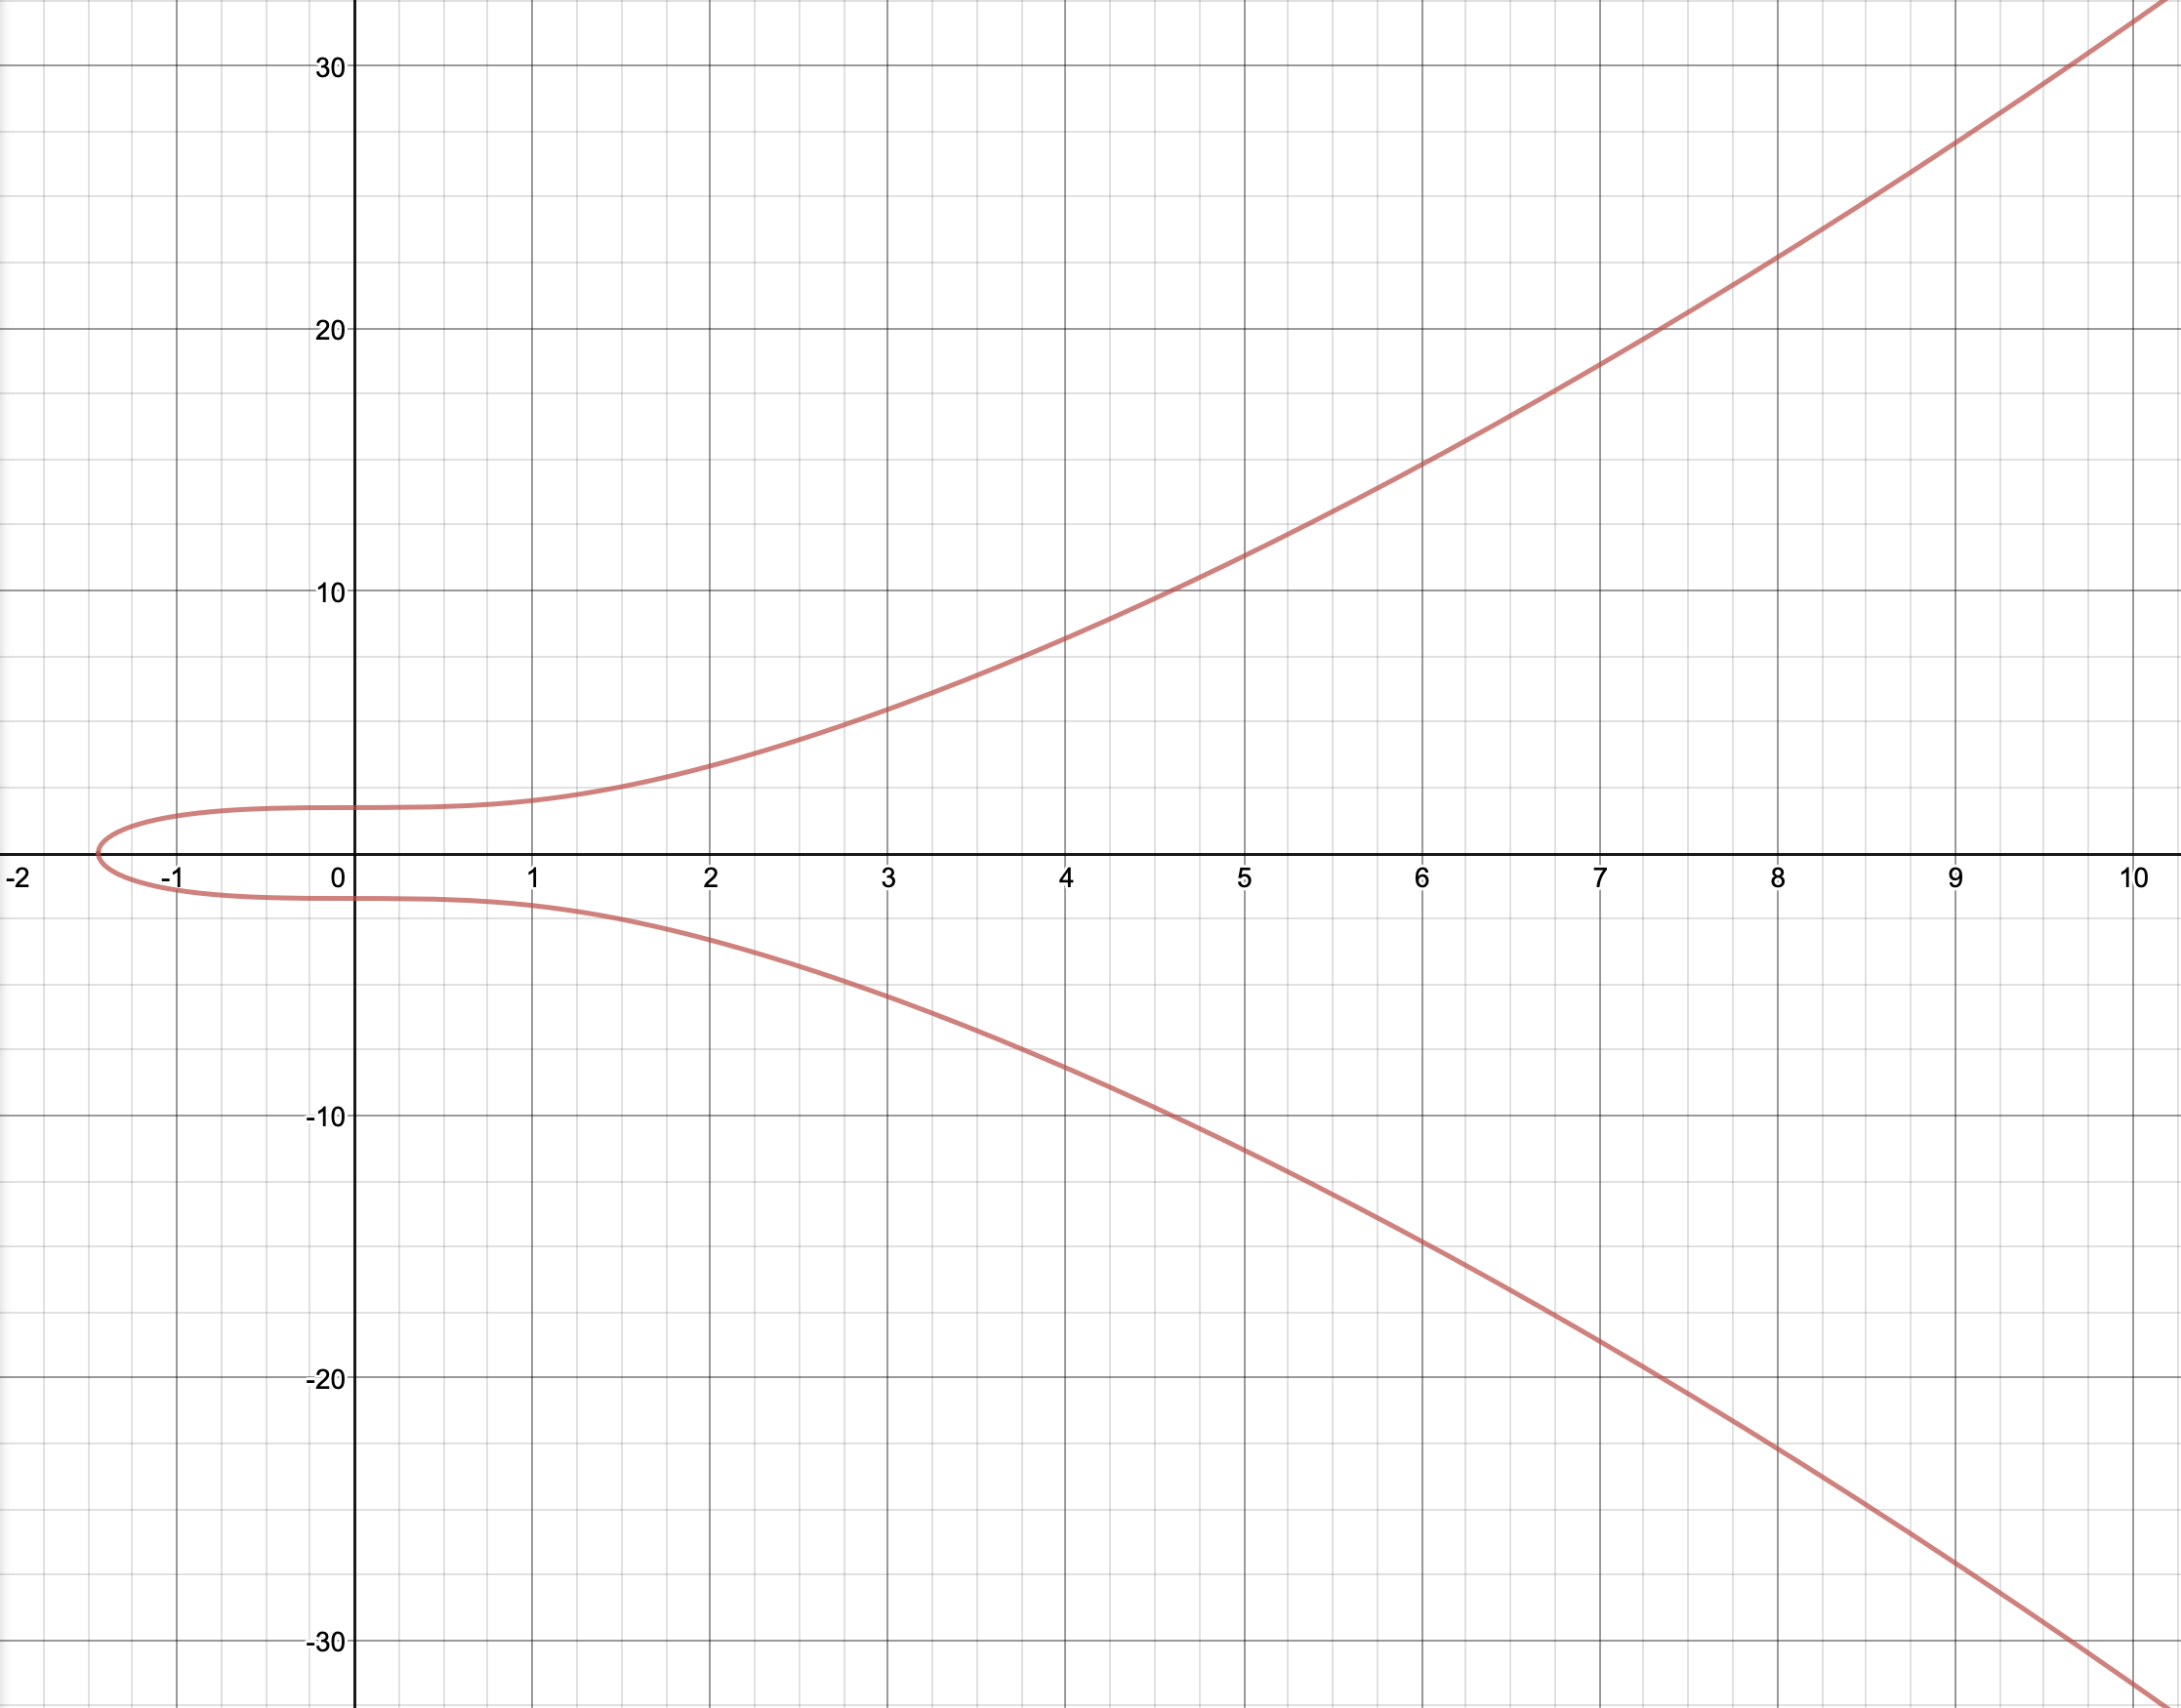
\includegraphics[width=0.8\textwidth]{images/ellipticCurveReals.png}
	\end{center}
	\caption{$y^2 = x^3 + 3$ over the real numbers.}
	\label{pic:ftShield}
\end{figure}

As an example, let's restrict the $x$ and $y$ coordinates to be the field of integers modulo $7$. I.e. we only allow the numbers $\mathbb{F}_7 = {0, 1, 2, 3, 4, 5, 6}$. In this world, $5 + 5 = 10 = 3\;(mod\;7)$.\\
\\
Let's consider the possible $y$-values of our elliptic curve $E$ when restricted to $\mathbb{F}_7$ (note: we write $E[\mathbb{F}_7]$ for 'the elliptic curve defined over the finite field $\mathbb{F}_7$).

\begin{tabular}{|c|c|c|c|c|c|c|c|}
    \hline
    $y$ & $0$ & $1$ & $2$ & $3$ & $4$ & $5$ & $6$ \\
    \hline
    $y^2$ & $0$ & $1$ & $4$ & $9=2$ & $16=2$ & $25=4$ & $36=1$ \\
    \hline
\end{tabular}

Now let's consider the $x$-values of $E[\mathbb{F}_7]$:

\begin{tabular}{|c|c|c|c|c|c|c|c|}
    \hline
    $x$ & $0$ & $1$ & $2$ & $3$ & $4$ & $5$ & $6$ \\
    \hline
    $x^3$ & $0$ & $1$ & $8=1$ & $27=6$ & $64=1$ & $125=6$ & $216=6$ \\
    \hline
    $x^3+3$ & $3$ & $4$ & $4$ & $9=2$ & $4$ & $9=2$ & $9=2$ \\
    \hline
    $= y^2$ & - & $4$ & $4$ & $2$ & $4$ & $2$ & $2$ \\
    \hline
    Valid $y$-values & 
        -- & 
        \makecell{$2$\\$5$} &
        \makecell{$2$\\$5$} &
        \makecell{$3$\\$4$} &
        \makecell{$2$\\$5$} &
        \makecell{$3$\\$4$} & 
        \makecell{$3$\\$4$} \\
    \hline
\end{tabular}

So we have a set of valid points of $\infty, (1,2), (1,5), (2,2), (2,5), (3,3), (3,4), (4,2), (4,5), (5,3), (5,4), (6,3), (6,4)$.\\
\\
These $13$ points are the only points which exist on $E[\mathbb{F}_7]$. $E[\mathbb{F}_7]$ is a `group' of order $13$.\\
In other words: the curve $E: y^2 = x^3 + 3$ --- when restricted to the $7$ values of $\mathbb{F}_7$ --- produces a group $E[\mathbb{F}_7]$ of order $13$.\\
\\
We superimpose the points of $E[\mathbb{F}_7]$ (in green) below:
\begin{figure}[H]
	\begin{center}
		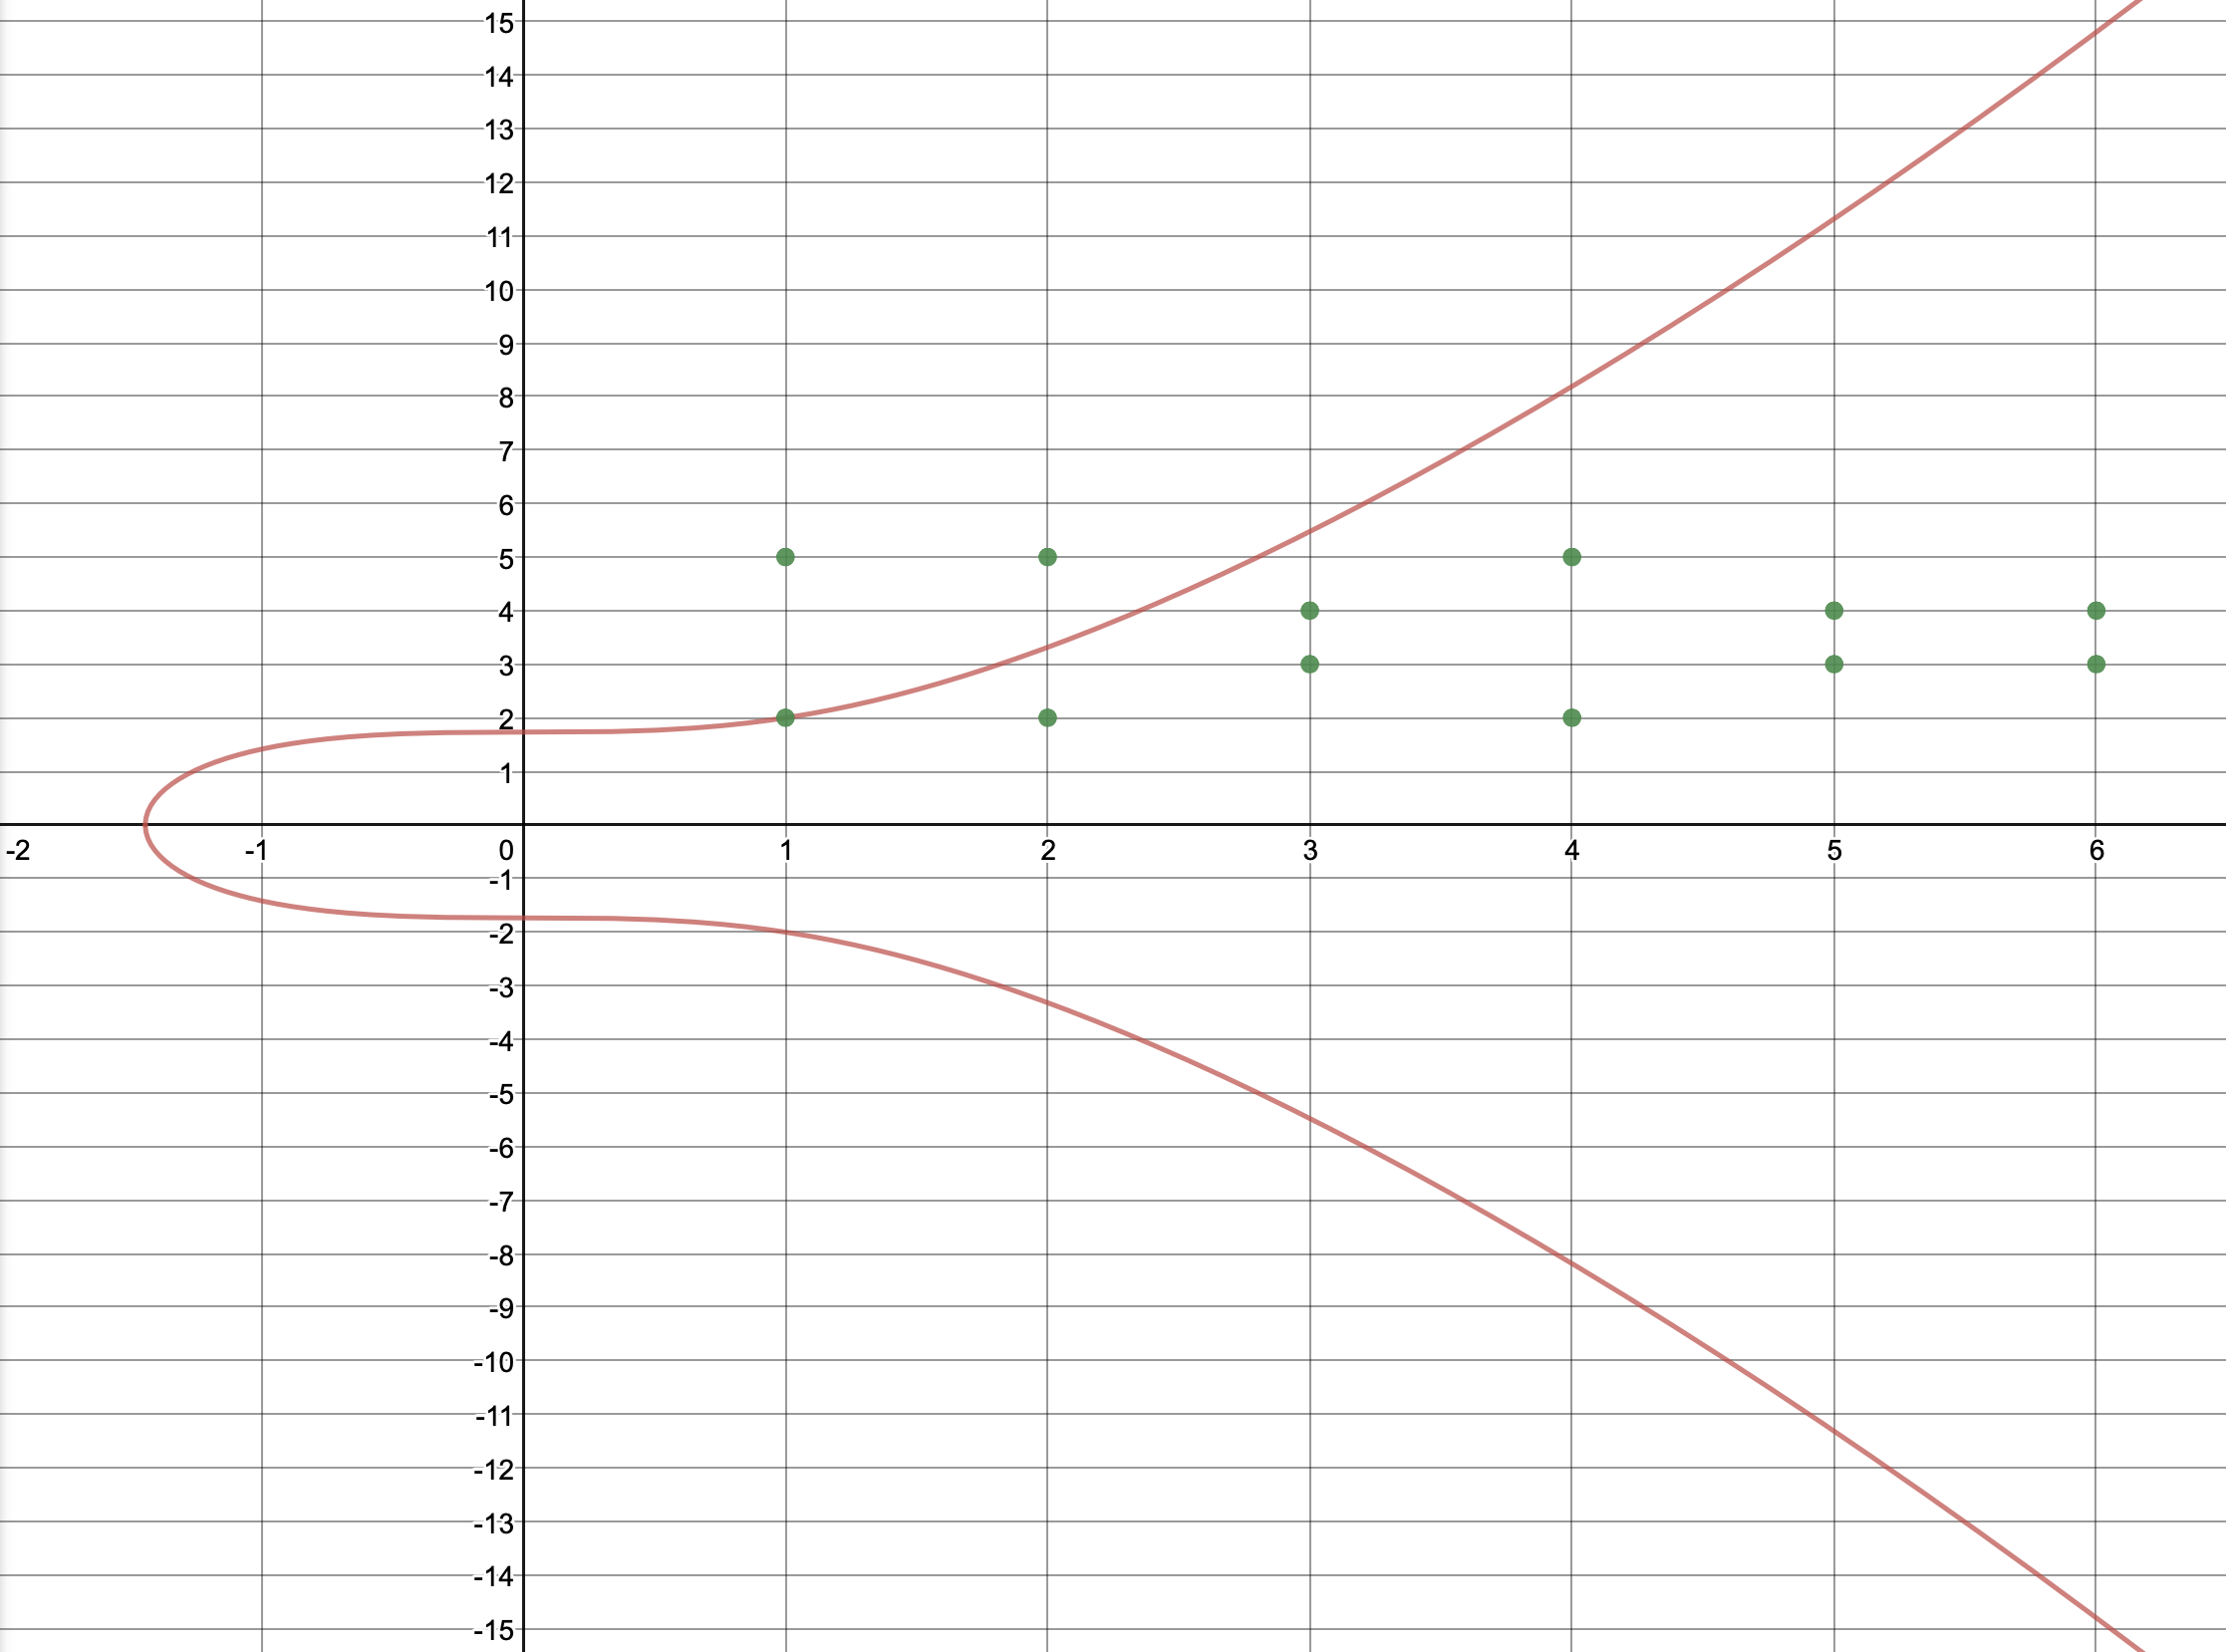
\includegraphics[width=0.8\textwidth]{images/ellipticCurveF7.png}
	\end{center}
	\caption{$y^2 = x^3 + 3$ over $\mathbb{F}_7$ shown as green dots.}
	\label{pic:ftShield}
\end{figure}

An important thing to take away from this example, is that there are 3 distinct things for us to be aware of: an elliptic curve equation $E$, a finite field $\mathbb{F}$, and the resulting group $G = E[\mathbb{F}]$. Sometimes the number of elements in the group $G$ is \textit{more than} the number of elements in the field $\mathbb{F}$ (as in the above example), and sometimes the number of elements in the group $G$ is \textit{less than} the number of elements in the field $\mathbb{F}$ (as we will see is the case with Ethereum).\\
\\
In practice, the finite field $\mathbb{F}_p$ used in Ethereum is of size
\begin{align*}
    p = 21888242871839275222246405745257275088696311157297823662689037894645226208583
\end{align*}

The elliptic curve $E: y^2 = x^3 + 3$, when restricted to the $p$ values of $\mathbb{F}_p$, produces a group $G_1 = E[\mathbb{F}_p]$ of prime order
\begin{align*}
    q = 21888242871839275222246405745257275088548364400416034343698204186575808495617
\end{align*}

I.e. $G_1 = E[\mathbb{F}_p]$ is a group with $q$ distinct points. Here, $q < p$; the size of the group $G_1$ is less than the size of the field $\mathbb{F_p}$.\\
\\
This has an important consequence when working within ZoKrates. To generate zk-SNARKs, ZoKrates will convert the numbers we pass as inputs to our off-chain calculation (as well as all intermediate numbers of the calculation) into elliptic curve points. To tie-in with Ethereum, ZoKrates converts all of the numbers used in its calculations into elements of the group $G_1$. Therefore, we need to make sure that \textbf{all} of the inputs we pass into ZoKrates are \textbf{less than} the size of the group $G_1$, $q = 21888242871839275222246405745257275088548364400416034343698204186575808495617$.\\
\\
This value of $q$ is slightly less than $254$-bits. I.e. $2^{253} < q < 2^{254}$.\\
\\
Hence, to be sure we don't `overflow' modulo-$q$, it's safest to only pass numbers to ZoKrates which are $\leq 253$-bits. When working with Ethereum, we often work with hex numbers (because Solidity `likes' hex numbers), which means it's often nice for the bit-length we work with to be divisible by $8$. Since $248$ is the largest number below $253$ which is divisible by $8$, this would have been a nice choice for all of the numbers Nightfall passes to ZoKrates.\\
\\
However, you might notice we instead restrict all our numbers to $216$-bits. The reason for this is the maximum size of a message in the NIST specification of the sha256 hashing algorithm. The largest message size for `one round' of sha256 hashing is $447$-bits. The version of ZoKrates used in Nightfall currently only supports `one round' of sha256 hashing. Hence our inputs to each hashing iteration must be $447$-bits or less.\\
\\
You'll see in the protocols below, that we frequently need to concatenate two values and then hash them. Hence we need each of the two values to be at most $223$-bits to fit inside `one round' of sha256 hashing. Given that we also prefer bit-lengths which are divisible by $8$, $216$-bits becomes the best choice for our purposes.\\
\\
\textbf{And that's why you'll see conversions and restrictions to 216-bit (27-byte) values in much of today's Nightfall code.}\\
\\
In cases where we need to use a number with a greater bit-length than $216$ (for security purposes), we deconstruct that number into an array of $216$-bit values. E.g. a $512$-bit number might be deconstructed into an array [$80$-bits, $216$-bits, $216$-bits].


%%%%%%%%%%%%%%%%%%%%%%%%%%%%%%%

\newpage
\part{The Protocols}
\label{part:theProtocols}
\parttoc

\newpage
\section{ERC-721 (non-fungible) tokens}
\label{sec:721}
\secttoc
\mtcskip
\sectlof

\newpage
\noindent
In this section we give an overview of using Nightfall to privately transact non-fungible tokens (nft's). We cover three key functions:
\begin{itemize}
	\item Mint - create an initial `token commitment'; a private representation of a public ERC-721 token.
	\item Transfer - nullify the sender's token commitment, and generate a new token commitment to represent ownership by the receiver.
	\item Burn - nullify a token commitment, and receive the underlying public ERC-721 token.
\end{itemize}

\subsubsection{Variables}
Here we describe the variables used in this section. 

\begin{center}
	\begin{tabular}{lp{14cm}}
    $A, B$      & Participants Alice and Bob.\\
    \\
    $pk_A$      & The public key belonging to Alice.\\
    $sk_A$      & The secret key belonging to Alice.\\
                & Note: there are several (secret key, public key) pairs in this protocol)\\
    \\
		$E_A$       & The Ethereum address of Alice.\\
		$\Xi_{A,i}$ & An `anonymous' Ethereum address belonging to Alice, where $i\in\mathbb{N}$ is an index, for distinguishing between multiple anonymous addresses. \\
    \\
    $\alpha$    & A unique representation of some non-fungible asset e.g. a tokenId in ERC-721.\\
                & Note that in respect of non-fungible tokens, Nightfall currently focusses solely ERC-721 tokens.
                  It would be relatively simple to adapt Nightfall's application to deal with other non-fungible token standards.\\
    $\alpha_A$  & A non-fungible asset $\alpha$ that is in Alice's possession. \\
    \\
		$\sigma$      & A salt used to provide uniqueness to commitment preimages.\\
		$\sigma_{\vec{AB}}$ & Stresses that a salt is being shared privately from Alice to Bob.\\
    \\
		$Z$         & An ERC-721 commitment; a zero-knowledge commitment representing ownership of some underlying ERC-721 asset. \\
    $Z_A$       & Stresses that an ERC-721 commitment belongs to Alice.\\
    $Z_{\alpha}$ & Stresses that an ERC-721 commitment represents the asset $\alpha$.\\
    $Z_{l}$     & Stresses that an ERC-721 commitment is the $l^{th}$ leaf of a Merkle Tree (see below for $M$).\\
                & Note that the meaning of these (seemingly colliding or ambiguous) subscripts will be clear from context.\\
    \\
    $N$         & A nullifier for an ERC-721 commitment $Z$.\\
    $N_A$       & A nullifier for the ERC-721 commitment $Z_A$.\\
    $N_{\alpha}$ & A nullifier for the ERC-721 commitment $Z_{\alpha}$.\\
    \\
		$M$         & A binary Merkle Tree.\\
    $M_l$       & A binary Merkle Tree with $l$ non-zero leaves (where leaves are populated in order `from left to right').\\
    $\roott_l$    & The root of $M_l$ (`$M$' is omitted because context will be clear).\\
    \\
    $\phi_{L}$  & $[\phi_{L}(d-1), \phi_{L}(d-2),..., \phi_{L}(1), \phi_{L}(0)]$ - The path from a leaf $L$ to the root of a Merkle Tree $M$, where $\phi_L(0) = \roott$.\\
    $\phi$      & $[\phi_{d-1}, \phi_{d-2},..., \phi_{1}, \phi_0]$ - Alternative notation for the path from a leaf, where the leaf $L$ is clear from the context. $\phi_0 = \roott$.\\
    $\psi_{L}$  & $[\psi_{L}(d-1), \psi_{L}(d-2),..., \psi_{L}(1), \psi_{L}(0)]$ - The sister-path from a leaf $L$ to the root of a Merkle Tree $M$, where $\psi_L(0) = \phi_L(0) = \roott$.\\
    $\psi$      &  $[\psi_{d-1}, \psi_{d-2},..., \psi_{1}, \psi_0]$ - Alternative notation for the sister-path from a leaf, where the leaf $L$ is clear from the context. $\psi_0 = \roott$.\\
    \\
		$x$         & Public inputs to a zk-SNARK. \\
		$\omega$    & Private inputs to a zk-SNARK.\\
		$C$         &  An arithmetic circuit $C: (\omega, x) \to \{0,1\}$.\\
		$p_C$       & A proving key for the circuit $C$. (Not to be confused with $pk$ which denotes a public key). \\
		$vk_C$      & A verification key for the circuit $C$. \\
    $\pi(p_C, x, \omega)$ & A proof for the circuit $C$, public inputs $x$, and private inputs $\omega$ \\
    $\pi_{C, x, \omega}$ & An abbreviation of the above. \\
    $\pi$       & An abbreviation of the above, when the context of the proof is clear. \\
    \\
    $h()$       & A one-way hashing function. Nightfall currently uses sha256 hashing throughout.\\
	\end{tabular}
\end{center}

\newpage
\subsubsection{Key Management}
\label{sec:721KeyManagement}
There are several pairs of public and private keys to keep track of throughout these protocols. We provide a summary here (for an actor Alice ($A$)):

\begin{center}
	\resizebox{\textwidth}{!}{
	\begin{tabular}{ c c c c c }
		\textbf{Ownership of...} & \textbf{Account symbol} & \textbf{Private Key} & \textbf{Public Key} & \textbf{Notes}\\
		\\
    \makecell{Ethereum address} & $E_A$ & $sk^E_A$ & $pk^E_A$ & Used for `mint' and `burn'. \\
		\\
    \makecell{Anonymous Ethereum addresses} & $\Xi_{A,i}$ & $sk^{\Xi}_{A,i}$ & $pk^{\Xi}_{A,i}$ & Used for `transfer'. $i\in\mathbb{N}$.\\
		\\
    \makecell{Ethereum Whisper accounts} & $W_{A,j}$ & $sk^{W}_{A,j}$ & $pk^{W}_{A,j}$ & Used for private messaging. $j\in\mathbb{N}$\\
		\\
    \makecell{ERC-721 commitment $Z_l$} & $Z_l$ & $sk^{Z,l}_{A}$ & $pk^{Z,l}_{A}$ & Used to `mint', `transfer' and `burn' $Z_l$.\\

	\end{tabular}
	}
\end{center}
\ \\
Hereafter, when we write $sk_A$ and $pk_A$ we will be referring to $sk^{Z,l}_{A}$ and $pk^{Z,l}_{A}$ respectively (where $Z_l$ is clear from context) - unless otherwise stated. 

\newpage
\subsection{Mint}
\label{sec:721Mint}

Suppose Alice wishes to be able to transfer ownership of an ERC-721 token under zero-knowledge, so that the following become private:

\begin{center}
  \begin{framed}
    \begin{enumerate}
      \item All details of the ERC-721 token (the `asset').
      \item The identity of the sender of the token (`Alice').
      \item The identity of the receiver of the token.
    \end{enumerate}
  \end{framed}
\end{center}

In order to achieve this, Alice must first convert her ERC-721 token into a private ERC-721 commitment. We call this act of conversion \textbf{`minting'} an ERC-721 commitment.
In this section, we outline Nightfall's protocol for minting an ERC-721 commitment, but first, an important privacy warning:

\begin{center}
  \begin{mdframed}[backgroundcolor=verylightred]
    \noindent
    PRIVACY WARNING\\
    \\
    \textit{
    Privacy is NOT achieved during the minting stage!
    }\\
    \\
    Minting an ERC-721 commitment initially requires Alice to transfer her ERC-721 token to a `Shield' contract (which thereafter holds it in escrow). This transfer reveals the Ethereum address of the sender (Alice) as well as the ERC-721 token itself. Therefore everyone will know the owner and the underlying asset being represented by the initial ERC-721 commitment which is created at this `minting' stage.\\
    \\
    Only during subsequent `transfers' of the new ERC-721 commitment, will we achieve the privacy intentions of Figure~\ref{fig:nfPrivacyIntentions}
  \end{mdframed}
\end{center}
\ \\
The ERC-721 standard allows many unique assets to be tokenised and represented by a unique tokenId within an ERC-721 smart contract.
Let $\alpha$ be the tokenId of some ERC-721 asset.\\
\\
For Alice to mint a token commitment representing $\alpha$, on the blockchain, under zero knowledge, she follows the steps in Figure~\ref{fig:nfMintAlgorithm}:

\begin{figure}[hp]
	\begin{center}
		\begin{framed}
      \begin{tabular}{p{16cm}}	
        \textbf{Non-fungible mint algorithm} \\
        \midrule
        \textbf{Alice's steps:}\\
        \begin{enumerate}
				  \item Generate a random salt $\sigma_{A}$.
				  \item Compute $Z_A := h(\;\alpha\;|\;pk^Z_A\;|\;\sigma_{A}\;)$, a token commitment which represents $\alpha$. 
          \item Set public inputs $x = (\;\alpha,\;Z_A\;)$
          \item Set private inputs $\omega = (\;pk_A^Z,\;\sigma_{A}\;)$
          \item Select $C_{nft\mbox{-}mint}(\;\omega,\;x\;)$ -- the set of constraints which are satisfied if and only if:
          \begin{enumerate}
            \item $Z_A$ equals $h(\;\alpha\;|\;pk_A^Z\;|\;\sigma_A\;)$ (Proof that the commitment $Z_A$ hides the correct asset $\alpha$)
          \end{enumerate}
          \item Generate $\pi := P(\;p_C\;,\;x,\;\omega\;)$; a proof of knowledge of satisfying arguments $(\omega, x)\;s.t.\;C(\omega, x) = 1$. Recall: $p_C$ -- the proving key for $C$ -- will be stored on Alice's computer.
           
          The pair $(\pi, x)$ is the zk-SNARK which attests to knowledge of private inputs $\omega$ without revealing them.
          \item Send $(\pi, x)$ to the Shield contract for verification.
           
          Using web3: \texttt{nfTokenShield.mint(proof, inputs, vkId)}
          %remember where the count (enumi) is up to and store it in ongoingEnumCounter:
          \setcounter{ongoingEnumCounter}{\value{enumi}}
        \end{enumerate}
        \ \\
        \midrule
        \textbf{Shield contract's steps:}\\
        \begin{enumerate}
          %resume counter
          \setcounter{enumi}{\value{ongoingEnumCounter}}
          \item Verify the proof as correct: call a Verifier contract to verify the \texttt{(proof, inputs)} pair against the verification key represented by \texttt{vkId}.
          \setcounter{ongoingEnumCounter}{\value{enumi}}
        \end{enumerate}
        \ \\
        \midrule
       \textbf{ Verifier contract's steps:}\\
        \begin{enumerate}
          \setcounter{enumi}{\value{ongoingEnumCounter}}
          \item Compute \texttt{result = verify(proof, inputs, vkId)}.
          
          I.e. Verify the \texttt{(proof, inputs)} pair against the verification key.
          \item Return \texttt{result}$\in$\texttt{\{false, true\}} to the Shield contract.
          \setcounter{ongoingEnumCounter}{\value{enumi}}
        \end{enumerate}
        \ \\
        \midrule
        \textbf{Shield contract's steps:}\\
        \begin{enumerate}
          \setcounter{enumi}{\value{ongoingEnumCounter}}
          \item If \texttt{result = false}, revert.
          \item Else:
          \begin{enumerate}
            \item Transfer $\alpha$ (the ERC-721 token with \texttt{tokenId} $=\alpha$), on behalf of Alice, to the Shield Contract. I.e. store $\alpha$ in escrow.
            \item Add $Z_A$ to the next empty leaf of the Merkle Tree.
            \item Recalculate the path to the root of the Merkle Tree from $Z_A$ for future users.
          \end{enumerate}
          \setcounter{ongoingEnumCounter}{\value{enumi}}
        \end{enumerate}
        \ \\
        \midrule
        \textbf{Alice's steps:}\\
        \begin{enumerate}
          \setcounter{enumi}{\value{ongoingEnumCounter}}
          \item Store relevant data in local database, including the leafindex of $Z_A$.
          \setcounter{ongoingEnumCounter}{0} %reset for next figure
        \end{enumerate} 
			\end{tabular}
		\end{framed}
	\end{center}
\caption{Non-Fungible Mint Algorithm}
\label{fig:nfMintAlgorithm}
\end{figure}

\newpage
\subsubsection{Details}
\label{sec:721MintDetails}

We refer to the numbered steps of Figure~\ref{fig:nfMintAlgorithm}.\\
\\
\textbf{Step $1$}
\ \\
This is handled within the \hyperref[sec:ui]{UI} microservice (or within the api-gateway).\\
\\
\textbf{Steps $2 - 4$}
\ \\
These steps are handled within \hyperref[sec:nf-token-controller]{\texttt{nf-token-controller.js}}.\\
\\
\textbf{Steps $5 - 6$}
\ \\
These steps are handled within a \hyperref[sec:zokrates]{ZoKrates} container.\\
\\
\textbf{Step $7$}
\ \\
This transaction is handled within \hyperref[sec:nf-token-zkp]{\texttt{nf-token-zkp.js}}.\\
\\
\textbf{Steps $8 - 10$}
\ \\
The Verifier contract already has stored within it the object $vk_C$ (see \hyperref[sec:trustedSetup]{Trusted Setup}). It runs a verification function $V(vk_C, \pi , x)$.
\begin{align*}
  V: (vk_C, \pi_{C,x,\omega}, x) \to \{0,1\}
\end{align*}
where:
\[
    V=
\begin{cases}
    1,& \text{if } \pi_{C,x,\omega} \text{ and } x \text{ satisfy } vk_C\\
    0,& \text{otherwise}
\end{cases}
\]

\textbf{Steps $11 - 12$}
\ \\
If the Verifier contract returns $1$ (\texttt{true}) (verified) to the Shield contract, then the Shield contract will be satisfied with Alice's commitment, and will update its persistent states:\\
\\
Suppose the Shield contract stores an ever-increasing array, $\bm{Z}$, of all token commitments which have ever been submitted by anyone.\\
\\
Suppose, prior to Alice's mint, there are $n-1$ tokens in the tree:
\begin{align*}
  \bm{Z}_{n-1} = (Z_0, Z_1, ..., Z_{n-1})
\end{align*}
The information held within $\bm{Z}_{n-1}$ may be represented by the root hash $\roott_{n-1}$ of a Merkle Tree $M_{n-1}$:\\


\begin{align*}
  \begin{forest}
    [{$\roott_{n-1}:= h\br*{
                      h\br*{
                        h\br*{
                          h\br*{
                            Z_0,Z_1
                          },
                          ...
                        },
                        h\br*{
                          h\br*{
                            Z_{n-1},0
                          },
                          0
                        }
                      },
                      0
                    }
                  $}
      [{$ h\br*{
            h\br*{
              h\br*{
                Z_0,Z_1
              },
              ...
            },
            h\br*{
              h\br*{
                Z_{n-1},0
              },
              0
            }
          }
        $}
        [{$ h\br*{
              h\br*{
                Z_0,Z_1
              },
              ...
            }
          $}
          [{$ h\br*{
                Z_0,Z_1
              }
            $}
            [{$Z_0$}][{$Z_1$}]
          ]
          [...
            [...][...]
          ]
        ]
        [{$ h\br*{
              h\br*{
                Z_{n-1},0
              },
              0
            }
          $}
          [{$ h\br*{
                Z_{n-1},0
              }
            $}
            [{$Z_{n-1}$}][0]
          ]
          [0
            [0][0]
          ]
        ]
      ]
      [0
        [0
          [0
            [0][0]
          ]
          [0
            [0][0]
          ]
        ]
        [0
          [0
            [0][0]
          ]
          [0
            [0][0]
          ]
        ]
      ]
    ]
  \end{forest}
\end{align*}

Now that the Shield contract has been given verification that Alice's commitment, $Z_A$, does indeed hide the asset $\alpha$, the Shield contract will do the following:\\

\begin{itemize}
  \item Append the commitment $Z_A$ to the ever-increasing array of tokens, $\bm{Z}_{n-1}$, so that $\bm{Z}_{n}=(Z_0, Z_1, ... Z_{n-1}, Z_A)$
  \item Recalculate a Merkle Root $\roott_{n}$ of $M_{n}$:
  \\
  \begin{align*}
    \begin{forest}
      [{$\roott_{n}:= h\br*{
                      h\br*{
                        h\br*{
                          h\br*{
                            Z_0,Z_1
                          },
                          ...
                        },
                        h\br*{
                          h\br*{
                            Z_{n-1},Z_A
                          },
                          0
                        }
                      },
                      0
                    }
                  $}
        [{$ h\br*{
              h\br*{
                h\br*{
                  Z_0,Z_1
                },
                ...
              },
              h\br*{
                h\br*{
                  Z_{n-1},Z_A
                },
                0
              }
            }
          $}
          [{$ h\br*{
                h\br*{
                  Z_0,Z_1
                },
                ...
              }
            $}
            [{$ h\br*{
                  Z_0,Z_1
                }
              $}
              [{$Z_0$}][{$Z_1$}]
            ]
            [...
              [...][...]
            ]
          ]
          [{$ h\br*{
                h\br*{
                  Z_{n-1},Z_A
                },
                0
              }
            $}
            [{$ h\br*{
                  Z_{n-1},Z_A
                }
              $}
              [{$Z_{n-1}$}][{$Z_A$}]
            ]
            [0
              [0][0]
            ]
          ]
        ]
        [0
          [0
            [0
              [0][0]
            ]
            [0
              [0][0]
            ]
          ]
          [0
            [0
              [0][0]
            ]
            [0
              [0][0]
            ]
          ]
        ]
      ]
    \end{forest}
  \end{align*}

  \item Append $\roott_{n}$ to an ever-increasing array $\rootsList=(\roott_0, \roott_1,..., \roott_{n-1}, \roott_{n})$
\end{itemize}
\ \\



\textbf{Step $13$}
\ \\
Alice will store all important information in her private database.



\newpage
\subsection{Transfer}
\label{sec:721Transfer}

\sectlof
We continue with the notation and indices from the `\hyperref[sec:Mint]{Mint}' section.\\
\\
Suppose Alice wishes to transfer ownership of the ERC-721 token with tokenId `$\alpha$' to Bob, but under zero-knowledge.\\
\\
In the `Mint' section, we saw how Alice can create an `ERC-721 commitment' $Z_\alpha$ within the Shield contract which:
\begin{itemize}
  \item hides an underlying ERC-721 token with tokenId `$\alpha$'; and
  \item hides and binds Alice as the owner of $Z_\alpha$ (and hence of $\alpha$) through an ownership keypair $(sk_A^Z, pk_A^Z)$.
\end{itemize}
\ \\
Recall our privacy intentions:\\
Alice wishes to be able to transfer ownership of an ERC-721 token under zero-knowledge, so that the following become private:
	\begin{center}
		\begin{framed}
      \begin{enumerate}
        \item All details of the ERC-721 token (the `asset').
        \item The identity of the sender of the token (`Alice').
        \item The identity of the receiver of the token.
      \end{enumerate}
    \end{framed}
  \end{center}
Recall that minting a token commitment does not yet afford Alice any privacy (see the warning in Figure~\ref{fig:nfMintWarning}). Only with subsequent transfers will the whereabouts of $\alpha$ and the owner of $\alpha$ be hidden.

For Alice to transfer ownership of $\alpha$ within the Shield contract, under zero knowledge, she follows the steps in Figure~\ref{fig:nfTransferAlgorithm}.

\begin{figure}[htbp]
  \ContinuedFloat*
	\begin{center}
		\begin{framed}
      \begin{tabular}{p{16cm}}	
       \textbf{ Non-fungible transfer algorithm} \\
        \\
        \midrule
        \textbf{Bob's steps:}\\
        \begin{enumerate}
          \item Before Alice can send him anything, Bob must register his public keys $pk_B^Z$ and $pk_B^W$ against both his public Ethereum address $pk_B^E$ and his unique name `Bob' within the \hyperref[sec:pkd]{PKD}.
          \setcounter{ongoingEnumCounter}{\value{enumi}}
        \end{enumerate}
        \ \\
        \midrule
        \textbf{Alice's steps:}\\
        \begin{enumerate}
          \setcounter{enumi}{\value{ongoingEnumCounter}}
          \item Generate a random salt $\sigma_{\vec{AB}}$.
          \item Lookup Bob's `zkp' public key $pk_B^Z$ from the PKD.
          \item Compute $Z_B := h(\;\alpha\;|\;pk^Z_B\;|\;\sigma_{\vec{AB}}\;)$, a token commitment which represents $\alpha$.
          \item Compute $N_A := h(\;\sigma_{A}\;|\;sk^Z_A\;)$, the nullifier of Alice's commitment $Z_A$.
          \item Get $\psi_{Z_A}$ -- the sister-path of $Z_A$ -- from the Shield contract (see Details below).
          \item Get the latest Merkle root from the Shield contract: $\roott_{n+m-1}$ (see Details below).
          \item Set public inputs $x = (\;N_A,\;\roott_{n+m-1},\;Z_B)$
          \item Set private inputs $\omega = (\alpha,\;\psi_{Z_A},\;sk_A,\;\sigma_{A},\;pk_B,\;\sigma_{\vec{AB}})$
          \item Select $C_{nft-transfer}(\;\omega,\;x\;)$ -- the set of constraints which are satisfied if and only if:
          \begin{enumerate}
            \item $pk_A$ equals $h(\;sk_A\;)$; (Proof of knowledge of the secret key to $pk_A$) (see Details for why $pk_A$ isn't an input to $C$)
            \item $Z_A$ equals $h(\;\alpha\;|\;pk_A\;|\;\sigma_A\;)$ (Proof of the constituent values of $Z_A$) (see Details for why $Z_A$ isn't an input to $C$)
            \item $\roott_{n+m-1}$ equals $h\br*{\psi_{1}\;|...|\;h\br*{\psi_{d-2}\;|\;h\br*{\psi_{d-1}\;|\;Z_A}\;}...}$ (Proof that $Z_A$ belongs to the on-chain Merkle Tree)
            \item $N_A$ equals $h(\;\sigma_{A}\;|\;sk^Z_A\;)$ (Proof $N_A$ is indeed the nullifier of $Z_A$)
            \item $Z_B$ equals $h(\;\alpha\;|\;pk^Z_B\;|\;\sigma_{\vec{AB}}\;)$ (Proof that $Z_B$ contains the same asset as $Z_A$)
          \end{enumerate}
          \item Generate $\pi := P(\;p_C\;,\;x,\;\omega\;)$; a proof of knowledge of satisfying arguments $(\omega, x)\;s.t.\;C(\omega, x) = 1$. Recall: $p_C$ -- the proving key for $C$ -- will be stored on Alice's computer.
           
          The pair $(\pi, x)$ is the zk-SNARK which attests to knowledge of private inputs $\omega$ without revealing them.
          \item Send $(\pi, x)$ to the Shield contract for verification.
           
          Using web3: \texttt{nfTokenShield.transfer(proof, inputs, vkId)}
          %remember where the count (enumi) is up to and store it in ongoingEnumCounter:
          \setcounter{ongoingEnumCounter}{\value{enumi}}
        \end{enumerate}
        \ \\
        \midrule
        \textbf{Shield contract's steps:}\\
        \begin{enumerate}
          %resume counter
          \setcounter{enumi}{\value{ongoingEnumCounter}}
          \item Verify the proof as correct: call a Verifier contract to verify the \texttt{(proof, inputs)} pair against the verification key represented by \texttt{vkId}.
          \setcounter{ongoingEnumCounter}{\value{enumi}}
        \end{enumerate}
        \ \\
        \hline
        ... 
			\end{tabular}
		\end{framed}
	\end{center}
\caption{Non-Fungible Transfer Algorithm}
\label{fig:nfTransferAlgorithm}
\end{figure}

%continue on next page
\begin{figure}[htbp]
  \ContinuedFloat %to continue
	\begin{center}
		\begin{framed}
      \begin{tabular}{p{16cm}}
       \textbf{ Verifier contract's steps:}\\
        \begin{enumerate}
          \setcounter{enumi}{\value{ongoingEnumCounter}}
          \item Compute \texttt{result = verify(proof, inputs, vkId)}.
          
          I.e. Verify the \texttt{(proof, inputs)} pair against the verification key.
          \item Return \texttt{result}$\in$\texttt{\{false, true\}} to the Shield contract.
          \setcounter{ongoingEnumCounter}{\value{enumi}}
        \end{enumerate}
        \ \\
        \midrule
        \textbf{Shield contract's steps:}\\
        \begin{enumerate}
          \setcounter{enumi}{\value{ongoingEnumCounter}}
          \item If \texttt{result = false}, revert.
          \item Else:
          \begin{enumerate}
            \item Check $\roott_{n+m-1}$ is in $\rootsList$. (Revert if not).
            \item Check $N_A$ is not already in its list of `spent' nullifiers. (Revert if not).
            \item Add $Z_B$ to the next empty leaf of the Merkle Tree.
            \item Recalculate the path to the root of the Merkle Tree from $Z_B$ for future users.
            \item Append the newly calculated root $\roott_{n+m}$ to the ever-increasing array $\rootsList$
            \item Similarly append the nullifier $N_{A}$ to the ever-increasing array $\bm N$.
          \end{enumerate}
          \setcounter{ongoingEnumCounter}{\value{enumi}}
        \end{enumerate}
        \ \\
        \midrule
        \textbf{Alice's steps:}\\
        \begin{enumerate}
          \setcounter{enumi}{\value{ongoingEnumCounter}}
          \item Store relevant data in her local database, including the leafindex of $Z_B$.
          \item Send Bob important data privately via Whisper (using his public key $pk^W_B$):
          \begin{enumerate}
            \item The salt $\sigma_{\vec{AB}}$ of $Z_B$.
            \item The public key of Bob, $pk^Z_B$, used by Alice in the preimage of $Z_B$ (for completeness, so Bob can check the correctness of $Z_B$ himself).
            \item The tokenId $\alpha$.
            \item $Z_B$.
            \item The leafIndex of $Z_B$ within the on-chain Merkle Tree $M$ (so Bob can locate it).
          \end{enumerate}
          \setcounter{ongoingEnumCounter}{\value{enumi}}
        \end{enumerate}
        \ \\
        \midrule
        \textbf{Bob's steps:}\\
        \begin{enumerate}
          \setcounter{enumi}{\value{ongoingEnumCounter}}
          \item Check the correctness of the information provided by Alice:
          \begin{enumerate}
            \item Check $Z_B$ equals $h(\;\alpha\;|\;pk^Z_B\;|\;\sigma_{\vec{AB}}\;)$
            \item Check that $Z_B$ is stored at the leafIndex of $M$ which Alice claimed.
          \end{enumerate}
          \item Store relevant data in his local database, including whether or not his `correctness checks' passed.
          \setcounter{ongoingEnumCounter}{0} %reset for next figure
        \end{enumerate} 
			\end{tabular}
		\end{framed}
	\end{center}
\caption{Non-Fungible Transfer Algorithm} %same caption as the first part of this figure
%\label{fig:nfTransferAlgorithm} - no label in this second part of the figure
\end{figure}


\newpage
\subsubsection{Details}
\label{sec:721TransferDetails}

We refer to the numbered steps of Figure~\ref{fig:nfTransferAlgorithm}.

\textbf{Step $1$}
\ \\
This is handled at the time Bob creates an account through the \hyperref[sec:ui]{UI}.\\
\\
\textbf{Step $2$}
\ \\
This is handled within the \hyperref[sec:ui]{UI} microservice (or within the api-gateway).\\
\\
\textbf{Step $3$}
\ \\
This is handled within the api-gateway when a call is made by Alice to transfer to Bob.\\
\\
\textbf{Steps $4 - 5$}
\ \\
These steps are handled within \hyperref[sec:nf-token-controller]{\texttt{nf-token-controller.js}}.\\
\\
\textbf{Steps $6 - 7$}
\ \\
These calls to the Shield contract are handled within \hyperref[sec:nf-token-zkp]{\texttt{nf-token-zkp.js}}.\\
\\
It is important at this stage to note that there are an unknown number of other parties utilising the Shield contract.
Hence, the dynamic array of tokens $\bm{Z}$ might have grown since Alice appended her $Z_A$ as the $n^{th}$ leaf of $M$ (during the \hyperref[sec:721Mint]{Mint} explanation).\\
Suppose there have been $m-1$ additional tokens added to $M$ since Alice added $Z_A$.
That is,\\
\begin{align*}
  \bm{Z}_{n+m-1} = (Z_0, Z_1,...,Z_{n-1}, Z_A, Z_{n+1},..., Z_{n+m-1})
\end{align*}
We denote the corresponding Merkle Tree which holds tokens $\bm{Z}_{n+m-1}$ by $M_{n+m-1}$.
We denote its root by $\roott_{n+m-1}$; an element of $\rootsList = (\roott_0, \roott_1,...,\roott_{n+m-1})$.\\
\\
\begin{align*}
  \begin{forest}
    [{$\roott_{n+m-1}:= h\br*{
                        h\br*{
                          h\br*{
                            h\br*{
                              Z_0,Z_1
                            },
                            ...
                          },
                          h\br*{
                            h\br*{
                              Z_{n-1},Z_A
                            },
                            h\br*{
                              Z_{n+1},...
                            }
                          }
                        },
                        h\br*{
                          h\br*{
                            h\br*{
                              Z_{n+m-1},0
                            },
                            0
                          },
                          0
                        }
                      }
                    $}
      [{$ h\br*{
            h\br*{
              h\br*{
                Z_0,Z_1
              },
              ...
            },
            h\br*{
              h\br*{
                Z_{n-1},Z_A
              },
              h\br*{
                Z_{n+1},...
              }
            }
          }
        $}
        [{$ h\br*{
              h\br*{
                Z_0,Z_1
              },
              ...
            }
          $}
          [{$ h\br*{
                Z_0,Z_1
              }
            $}
            [{$Z_0$}][{$Z_1$}]
          ]
          [...
            [...][...]
          ]
        ]
        [{$ h\br*{
              h\br*{
                Z_{n-1},Z_A
              },
              h\br*{
                Z_{n+1},...
              }
            }
          $}
          [{$ h\br*{
                Z_{n-1},Z_A
              }
            $}
            [{$Z_{n-1}$}][{$Z_A$}]
          ]
          [{$ h\br*{
                Z_{n+1},...
              }
            $}
            [$Z_{n+1}$][...]
          ]
        ]
      ]
      [{$ h\br*{
            h\br*{
              h\br*{
                Z_{n+m-1},0
              },
              0
            },
            0
          }
        $}
        [{$ h\br*{
              h\br*{
                Z_{n+m-1},0
              },
              0
            }
          $}
          [{$ h\br*{
                Z_{n+m-1},
                0
              }
            $}
            [{$Z_{n+m-1}$}][0]
          ]
          [0
            [0][0]
          ]
        ]
        [0
          [0
            [0][0]
          ]
          [0
            [0][0]
          ]
        ]
      ]
    ]
  \end{forest}
\end{align*}

\noindent
Alice retrieves the value of the current Merkle root, $\roott_{n+m-1}$, from the Shield contract.\\
\\
Since Alice knows that $Z_A$ is at leaf-index $n$ of $M_{n+m-1}$, Alice can also retrieve the path from the leaf $Z_{n}=Z_A$ to the root $\roott_{n+m-1}$. Path computations are done in \texttt{zkp/src/format-inputs.js}.\\
\\
We denote this path:
\begin{align*}
  \phi_{Z_A} = [\phi_{d-1}, \phi_{d-2},..., \phi_{1}, \phi_0]
\end{align*}
Note that $\phi_0 = \roott_{n+m-1}$.\\
\\
Alice also retrieve's the `sister-path' of this path:
\begin{align*}
  \psi_{Z_A} = [\psi_{d-1}, \psi_{d-2},..., \psi_{1}, \psi_0]
\end{align*}
where $\psi_0 = \phi_0 = \roott_{n+m-1}$\\
\\
For ease of reading, let's focus only on the nodes of $M_{n+m-1}$ which Alice cares about for the purposes of transferring to Bob:

\begin{align*}
  \begin{forest}
    [{$\roott_{n+m-1}:=\phi_0=\psi_0$}
      [{$\phi_1$}
        [{$\psi_2$}
          [...
            [...][...]
          ]
          [...
            [...][...]
          ]
        ]
        [{$\phi_2$}
          [{$\phi_3$}
            [{$\psi_4$}][{$Z_A$}]
          ]
          [{$\psi_3$}
            [...][...]
          ]
        ]
      ]
      [{$\psi_1$}
        [...
          [...
            [...][0]
          ]
          [0
            [0][0]
          ]
        ]
        [0
          [0
            [0][0]
          ]
          [0
            [0][0]
          ]
        ]
      ]
    ]
  \end{forest}
\end{align*}


\noindent
Equipped with $\psi_{Z_A}$, Alice can prove that she owns a token commitment at one of the leaves of $M_{n+m-1}$, without revealing that it is "$Z_n$ located at leaf-index $n$".\\
\\
\textbf{Steps $8 - 9$}
\ \\
These steps are handled within \hyperref[sec:nf-token-controller]{\texttt{nf-token-controller.js}}.\\
\\
As a reminder, we let:
\begin{center}
  \begin{tabular}{l l}
    $x = (N_{A},\
          \roott_{n+m-1},\
          Z_B)$ & Public Inputs used to generate the Proof\\
    $\omega = (\alpha,\
              \psi_{Z_A},\
              sk_A,\
              \sigma_{A},\
              pk_B,\
              \sigma_{\vec{AB}})$ & Private Inputs used to generate the Proof\\
  \end{tabular}
\end{center}
\ \\
\textbf{Steps $10 - 11$}
\ \\
These steps are handled within a \hyperref[sec:zokrates]{ZoKrates} container.\\
\\
Alice uses the $C_{nft-transfer}$ (or $C$) -- the set of constraints for a non-fungible transfer, located in \texttt{zkp/code/gm17/nft-transfer} (see \hyperref[sec:trustedSetup]{Trusted Setup}). $C_{nft-transfer}(\;\omega,\;x\;)$ returns a value of $true$ if Alice provides a set of valid `satisfying' arguments $(\omega, x)$ to $C$.\\
\\
Let's elaborate on each of the checks and calculations constraining the inputs to $C$ (we highlight public inputs in \textbf{bold} below):
\begin{enumerate}
  \item Calculate $h(sk_A) =: pk_A'$.\\
    Note that this newly calculated $pk_A'$ should equal $pk_A$ (Alice's public key), but we don't need to pass $pk_A$ as a private input and explicitly check that $pk_A'=pk_A$; a check on the correctness of $sk_A$ (and hence $pk_A'$) is implicitly achieved in the next two steps:
  \item Calculate $h(\alpha\;|\;pk_A'\;|\;\sigma_A) =: Z_A'$.\\
    Note again that this newly calculated $Z_A'$ should equal $Z_A$ (Alice's token commitment), but we don't need to pass $Z_A$ as a private input and explicitly check that $Z_A'=Z_A$; a check on the correctness of $Z_A$ (and hence $Z_A'$) is implicitly achieved in the next step:
  \item Check inputs $\psi_{Z_A}=[\psi_{d-1}, \psi_{d-2},..., \psi_{1}, \bm{\psi_{0}=\roott_{n+m-1}}]$ and the newly calculated $Z_A'$ satisfy:\\
    $h\br*{\psi_{1}\;|...|\;h\br*{\psi_{d-2}\;|\;h\br*{\psi_{d-1}\;|\;Z_A'}\;}...} = \roott_{n+m-1} ( =: \bm{\psi_{0}})$\\
    Given the one-way nature of our hashing function $h$, the only feasible way we could have arrived at the correct value of $\roott_{n+m-1}$ is if the sister-path $\psi_{Z_A}$ is correct, and if $Z_A'$ is correct, which (working backwards) must mean that $sk_A$ is correct.

    How does the circuit know the value of $\roott_{n+m-1}$ is correct? It doesn't; but it is a `public input', and we can rely upon the Shield smart contract to check the correctness of all public inputs.\\
  \\
  We've therefore shown in the steps so far, that:
  \begin{itemize}
    \item[--] Alice is the owner of a token commitment (because she knows its secret key)
    \item[--] Said token commitment is indeed a leaf of the on-chain Merkle Tree $M_{n+m-1}$.
  \end{itemize}

  Alice commits to spending her token $Z_A$ in the next step:
  \item Check inputs $\sigma_{A}, sk_A, \bm{N_A}$ satisfy:
    $h(\sigma_{A}\;|\;sk_A) = \bm{N_{A}}$\\
    $N_A$ is referred to as a `nullifier' because it is understood by all participants to be an indisputable commitment to spend (`nullify') a token commitment. Remember that the token commitment being spent isn't revealed; the earlier steps have allowed Alice to demonstrate hidden knowledge of the secret key $sk_A$ of a token commitment which does indeed exist. By including $sk_A$ in the nullifier's preimage, Alice is binding herself as the executor of this transfer. By including $\sigma_A$, Alice is specifying a serial number which is unique to the token $Z_A$ (thereby distinguishing this nullifier from those which would nullify any other token commitments she may own).\\
  \item Check inputs $\alpha, pk_B, \sigma_{\vec{AB}}, \bm{Z_B}$ satisfy:
    $h(\alpha\;|\;pk_B\;|\;\sigma_{\vec{AB}}) = \bm{Z_B}$\\
    This final step constrains the same asset $\alpha$ to be included in $Z_B$ as was included in $Z_A$.\\
    You might notice that the circuit doesn't actually constrain Alice to use the correct values for Bob's public key $pk_B$, nor the serial number $\sigma_{\vec{AB}}$ as inputs to the circuit. Alice is free to transfer ownership of the token commitment to anyone.
\end{enumerate}
Notice how each stage is linked to the last, and that at each of the `Check' stages, private inputs are being reconciled against at least one public input (highlighted in \textbf{bold} to help you notice). By structuring the circuit $C$ in this way, we are able to share only the public inputs with the Shield contract (along with a `proof' $\pi_{C,x,\omega}$). We'll see shortly that the Shield contract checks the correctness of each of the public inputs against its current states.\\
\\

\noindent
If all of the above constraints are satisfied by the public and private inputs, ZoKrates will generate the proof $\pi_{C,x,\omega}$; a proof of knowledge of satisfying arguments $(\omega, x) \ s.t. \ C(\omega, x) = 1$.\\
\\
\textbf{Step $12$}
\ \\
This transaction is handled within \hyperref[sec:nf-token-zkp]{\texttt{nf-token-zkp.js}}.\\
\\
Having generated $\pi_{C,x,\omega}$, Alice then sends the following to the Shield contract from her anonymous Ethereum address $\Xi_{A,1}$:
\begin{align*}
  &\pi_{C,x,\omega}\\
  &x = (N_{A}, \roott_{n+m-1}, Z_B)
\end{align*}
\\
Recall that everyone knows the checks and calculations which have been performed in the circuit $C_{nft-transfer}$, because it is a public file in the Nightfall repository. Further, everyone knows the verification key $vk_C$ which uniquely represents this circuit, because it has been publicly stored in the Verifier Registry contract. Therefore, when this anonymous caller (Alice) shares the pair $(x, \pi_{C,x,\omega})$, and the `unique id' of the relevant verification key $vk_C$; everyone will interpret this information as the caller's intention to transfer, and everyone will be convinced that the caller knows the secret key which permits them to transfer ownership of a token commitment.\\
\\



\textbf{Steps $13 - 15$}
\ \\
The Verifier Registry contract already has stored within it the verification key $vk_C$.
It runs a verification function $V(vk_C, \pi_{C,x,\omega}, x)$.
\begin{align*}
  V: (vk_C, \pi_{C,x,\omega}, x) \to \{0,1\}
\end{align*}
where:
\[
    V=
\begin{cases}
    1,& \text{if } \pi_{C,x,\omega} \text{ and } x \text{ satisfy } vk_C\\
    0,& \text{otherwise}
\end{cases}
\]
\ \\


\textbf{Steps $16 - 17$}
\ \\
If the Verifier contract returns $1$ ($true$) (verified) to the Shield contract, then the Shield contract will be satisfied that Alice's proof and public inputs represent her commitment to relinquish ownership of a token commitment, and to transfer ownership of the underlying asset to someone via the newly proposed token commitment $Z_B$. If the Verifier contract returns $0$, then the transaction will revert.\\
\\
Let's suppose Alice's $(x, \pi_{C,x,\omega})$ pair is verified.\\
\\
Following verification of the proof, the Shield contract will do the following:
\begin{enumerate}
  \item Check $\roott_{n+m-1}$ is in $\rootsList$.\\
    (If not, the transfer will fail)
  \item Check $N_A$ is not already in the list of nullifiers, which we denote $\bm{N}$.\\
    (If $N_A$ is already in $\bm{N}$, the transfer will fail)
  \item Append the commitment $Z_B$ to the ever-increasing array of tokens, $\bm{Z}_{n+m}$, so that $\bm{Z}_{n+m}=(Z_0, Z_1, ... Z_{n-1}, Z_A, Z_{n+1}, ... Z_{n+m-1}, Z_B)$\\
  \item Recalculate a Merkle Root $\roott_{n+m}$ of $M_{n+m}$\\
    \\
    \begin{align*}
      \begin{forest}
        [{$\roott_{n+m}:= h\br*{
                            h\br*{
                              h\br*{
                                h\br*{
                                  Z_0,Z_1
                                },
                                ...
                              },
                              h\br*{
                                h\br*{
                                  Z_{n-1},Z_A
                                },
                                h\br*{
                                  Z_{n+1},...
                                }
                              }
                            },
                            h\br*{
                              h\br*{
                                h\br*{
                                  Z_{n+m-1}, Z_B
                                },
                                0
                              },
                              0
                            }
                          }
                        $}
          [{$ h\br*{
                h\br*{
                  h\br*{
                    Z_0,Z_1
                  },
                  ...
                },
                h\br*{
                  h\br*{
                    Z_{n-1},Z_A
                  },
                  h\br*{
                    Z_{n+1},...
                  }
                }
              }
            $}
            [{$ h\br*{
                  h\br*{
                    Z_0,Z_1
                  },
                  ...
                }
              $}
              [{$ h\br*{
                    Z_0,Z_1
                  }
                $}
                [{$Z_0$}][{$Z_1$}]
              ]
              [...
                [...][...]
              ]
            ]
            [{$ h\br*{
                  h\br*{
                    Z_{n-1},Z_A
                  },
                  h\br*{
                    Z_{n+1},...
                  }
                }
              $}
              [{$ h\br*{
                    Z_{n-1},Z_A
                  }
                $}
                [{$Z_{n-1}$}][{$Z_A$}]
              ]
              [{$ h\br*{
                    Z_{n+1},...
                  }
                $}
                [$Z_{n+1}$][...]
              ]
            ]
          ]
          [{$ h\br*{
                h\br*{
                  h\br*{
                    Z_{n+m-1}, Z_B
                  },
                  0
                },
                0
              }
            $}
            [{$ h\br*{
                  h\br*{
                    Z_{n+m-1}, Z_B
                  },
                  0
                }
              $}
              [{$ h\br*{
                    Z_{n+m-1}, Z_B
                  }
                $}
                [{$Z_{n+m-1}$}][{$Z_B$}]
              ]
              [0
                [0][0]
              ]
            ]
            [0
              [0
                [0][0]
              ]
              [0
                [0][0]
              ]
            ]
          ]
        ]
      \end{forest}
    \end{align*}

    Note that the Shield contract only needs to calculate the hashes on the path from $Z_B$ to the root.

  \item Append $\roott_{n+m}$ to the ever-increasing array $\rootsList$
  \item Similarly append the nullifier $N_{A}$ to the ever-increasing array $\bm N$.
\end{enumerate}
\ \\

\textbf{Steps $18 - 19$}
\ \\
The api-gateway routes the data resulting from a transfer to her local database.\\
\\
Similarly, the api-gateway ensures any sensitive data (data which is private to Alice alone) is filtered before Alice sends data to Bob.\\
\\
Data which is crucial to Bob verifying his ownership of the new $Z_B$ is encrypted with Bob's public whisper key $pk^W_B$ and broadcast to the Whisper network.\\
\\

\textbf{Steps $20 - 21$}
\ \\
Nightfall uses web3.shh to use Whisper. Bob's logged-in application will listen for all Whisper messages, and will try to decrypt all messages with his private whisper key $sk^W_B$. If decryption is successful, the data will be stored in the relevant database on Bob's local machine.\\
\\
\hyperref[sec:nf-token-zkp]{\texttt{nft-token-zkp.js}} includes functions to cross-reference the data Bob has received from Alice against the data stored in the Shield contract.\\
\\
Bob will store all important information in his private database.



\newpage
\subsection{Burn}
\label{sec:721Burn}

We continue with the notation and indices from the prior sections.\\
\\
Suppose Bob is the owner of the token commitment $Z_B$ which represents the ERC-721 asset with tokenId $\alpha$ (as discussed in the prior section).
The asset $\alpha$ can continue to be transferred under zero-knowledge between parties within the Shield contract indefinitely.
Any third-party observers would not be able to infer "who sent what to whom".\\
\\
Recall that whilst the ERC-721 token represented by $\alpha$ has a `private' token commitment representation within the Shield contract, the underlying `public' ERC-721 token is owned by the Shield contract; effectively `locked up' in escrow.\\
\\
Suppose Bob (now the owner of $\alpha$ because he knows the secret key $sk^{Z,(n+m+1)}_{B,0}$) wishes to `release' his public ERC-721 token represented by $\alpha$ from escrow.
Then he will need to effectively `reveal' the contents of his token commitment $Z_B$ in order to convince the Shield contract that he is indeed entitled to withdraw $\alpha$ from escrow.
We call this act of converting from a `private' token commitment back to its `public' counterpart a `\textbf{burn}'.\\
\\
Note that by burning a token commitment, Bob is revealing information which was previously private; namely, the asset $\alpha$. Bob could continue to use an anonymous Ethereum address when calling the `burn' transaction, but analytics of public ERC-721 transactions thereafter will likely eventually reveal that it was Bob who burned $\alpha$. We'll have Bob use his public Ethereum address `burn', for simplicity.\\
\\

\noindent
For Bob to burn $Z_B$ within the Shield contract, under zero knowledge, he follows the steps in Figure~\ref{fig:nfBurnAlgorithm}.

\begin{figure}[htp]
  \ContinuedFloat*
	\begin{center}
		\begin{framed}
      \begin{tabular}{p{16cm}}	
        \textbf{Non-fungible burn algorithm} \\
        \\
        \midrule
        \textbf{Bob's steps:}\\
        \begin{enumerate}
          \setcounter{enumi}{\value{ongoingEnumCounter}}
          \item Compute $N_B := h(\;\sigma_{\vec{AB}}\;|\;sk^Z_B\;)$, the nullifier of Bob's commitment $Z_B$.
          \item Get $\psi_{Z_B}$ -- the sister-path of $Z_B$ -- from the Shield contract (see Details below).
          \item Get the latest Merkle root from the Shield contract: $\roott_{n+m+k-1}$ (see Details below).
          \item Set public inputs $x = (\alpha,\;N_B,\;\roott_{n+m+k-1})$
          \item Set private inputs $\omega = (\psi_{Z_A},\;sk_B,\;\sigma_{\vec{AB}})$
          \item Select $C_{nft-burn}(\;\omega,\;x\;)$ -- the set of constraints which are satisfied if and only if:
          \begin{enumerate}
            \item $pk_B$ equals $h(\;sk_B\;)$; (Proof of knowledge of the secret key to $pk_B$) (see Details for why $pk_B$ isn't an input to $C$)
            \item $Z_B$ equals $h(\;\alpha\;|\;pk_B\;|\;\sigma_{\vec{AB}}\;)$ (Proof of the constituent values of $Z_B$) (see Details for why $Z_B$ isn't an input to $C$)
            \item $\roott_{n+m+k-1}$ equals $h\br*{\psi_{1}\;|...|\;h\br*{\psi_{d-2}\;|\;h\br*{\psi_{d-1}\;|\;Z_B}\;}...}$ (Proof that $Z_B$ belongs to the on-chain Merkle Tree)
            \item $N_B$ equals $h(\;\sigma_{\vec{AB}}\;|\;sk^Z_B\;)$ (Proof $N_B$ is indeed the nullifier of $Z_B$)
          \end{enumerate}
          \item Generate $\pi := P(\;p_C\;,\;x,\;\omega\;)$; a proof of knowledge of satisfying arguments $(\omega, x)\;s.t.\;C(\omega, x) = 1$. Recall: $p_C$ -- the proving key for $C$ -- will be stored on Alice's computer.
           
          The pair $(\pi, x)$ is the zk-SNARK which attests to knowledge of private inputs $\omega$ without revealing them.
          \item Send $(\pi, x)$ to the Shield contract for verification.
           
          Using web3: \texttt{nfTokenShield.burn(payTo, proof, inputs, vkId)}

          where \texttt{payTo} is an Ethereum address, specified by Bob, into which he wishes for the ERC-721 token with tokenId $=\alpha$ to be transferred.
          %remember where the count (enumi) is up to and store it in ongoingEnumCounter:
          \setcounter{ongoingEnumCounter}{\value{enumi}}
        \end{enumerate}
        \ \\
        \midrule
        \textbf{Shield contract's steps:}\\
        \begin{enumerate}
          %resume counter
          \setcounter{enumi}{\value{ongoingEnumCounter}}
          \item Verify the proof as correct: call a Verifier contract to verify the \texttt{(proof, inputs)} pair against the verification key represented by \texttt{vkId}.
          \setcounter{ongoingEnumCounter}{\value{enumi}}
        \end{enumerate}
        \ \\
        \hline
        ... 
			\end{tabular}
		\end{framed}
	\end{center}
\caption{Non-Fungible Burn Algorithm}
\label{fig:nfBurnAlgorithm}
\end{figure}

%continue on next page
\begin{figure}[htp]
  \ContinuedFloat %to continue
	\begin{center}
		\begin{framed}
      \begin{tabular}{p{16cm}}
        \textbf{Verifier contract's steps:}\\
        \begin{enumerate}
          \setcounter{enumi}{\value{ongoingEnumCounter}}
          \item Compute \texttt{result = verify(proof, inputs, vkId)}.
          
          I.e. Verify the \texttt{(proof, inputs)} pair against the verification key.
          \item Return \texttt{result}$\in$\texttt{\{false, true\}} to the Shield contract.
          \setcounter{ongoingEnumCounter}{\value{enumi}}
        \end{enumerate}
        \ \\
        \midrule
        \textbf{Shield contract's steps:}\\
        \begin{enumerate}
          \setcounter{enumi}{\value{ongoingEnumCounter}}
          \item If \texttt{result = false}, revert.
          \item Else:
          \begin{enumerate}
            \item Check $\roott_{n+m+k-1}$ is in $\rootsList$. (Revert if not).
            \item Check $N_B$ is not already in its list of `spent' nullifiers. (Revert if not).
            \item Transfer the ERC-721 token with tokenId $=\alpha$ from the Shield contract (which has been holding it in escrow) to Bob's \texttt{payTo} Ethereum address.
            \item Append the nullifier $N_{B}$ to the ever-increasing array $\bm N$.
          \end{enumerate}
          \setcounter{ongoingEnumCounter}{\value{enumi}}
        \end{enumerate}
        \ \\
        \midrule
        \textbf{Bob's steps:}\\
        \begin{enumerate}
          \setcounter{enumi}{\value{ongoingEnumCounter}}
          \item Check the ERC-721 contract to ensure he owns the token with tokenId $=\alpha$.
          \item Store any relevant data in his local database.
          \setcounter{ongoingEnumCounter}{0} %reset for next figure
        \end{enumerate} 
			\end{tabular}
		\end{framed}
	\end{center}
\caption{Non-Fungible Burn Algorithm} %same caption as the first part of this figure
%\label{fig:nfBurnAlgorithm} - no label in this second part of the figure
\end{figure}




\newpage
\subsubsection{Details}
\label{sec:721BurnDetails}

We refer to the numbered steps of Figure~\ref{fig:nfBurnAlgorithm}.\\
\\

\textbf{Step $1$}
\ \\
This is handled within \hyperref[sec:nf-token-controller]{\texttt{nf-token-controller.js}}.\\
\\

\textbf{Steps $2 - 3$}
\ \\
These calls to the Shield contract are handled within \hyperref[sec:nf-token-zkp]{\texttt{nf-token-zkp.js}}.\\
\\
\noindent
It is important at this stage to note that there are an unknown number of other parties utilising the Shield smart contract.
Hence, the dynamic array of tokens $\bm{Z}$ might have grown since Alice appended Bob's $Z_B$ as the $(n+m)^{th}$ leaf of $M$.\\
\\
Suppose there have been $k-1$ additional tokens added to $\bm{Z}$ since Alice added Bob's $Z_B$.
That is,\\
\begin{align*}
  \bm{Z}_{n+m+k-1} = (Z_0, Z_1,..., Z_{n-1}, Z_A,
  Z_{n+1},..., Z_{n+m-1}, Z_B, Z_{n+m+1},..., Z_{n+m+k-1})
\end{align*}
\ \\
\noindent
We denote the corresponding Merkle Tree which holds tokens $\bm{Z}_{n+m+k-1}$ by $M_{n+m+k-1}$. We denote its root by $\roott_{n+m+k-1}$; an element of $\rootsList$.



\begin{align*}
  \scalebox{0.9}{
    \begin{forest}
      [{$\roott_{n+m+k-1}:= h\br*{
                          h\br*{
                            h\br*{
                              h\br*{
                                Z_0,Z_1
                              },
                              ...
                            },
                            h\br*{
                              h\br*{
                                Z_{n-1},Z_A
                              },
                              h\br*{
                                Z_{n+1},...
                              }
                            }
                          },
                          h\br*{
                            h\br*{
                              h\br*{
                                Z_{n+m-1}, Z_B
                              },
                              h\br*{
                                Z_{n+m+1}, ...
                              }
                            },
                            h\br*{
                              h\br*{
                                Z_{n+m+k-1}, 0
                              },
                              0
                            }
                          }
                        }
                      $}
        [{$ h\br*{
              h\br*{
                h\br*{
                  Z_0,Z_1
                },
                ...
              },
              h\br*{
                h\br*{
                  Z_{n-1},Z_A
                },
                h\br*{
                  Z_{n+1},...
                }
              }
            }
          $}
          [{$ h\br*{
                h\br*{
                  Z_0,Z_1
                },
                ...
              }
            $}
            [{$ h\br*{
                  Z_0,Z_1
                }
              $}
              [{$Z_0$}][{$Z_1$}]
            ]
            [...
              [...][...]
            ]
          ]
          [{$ h\br*{
                h\br*{
                  Z_{n-1},Z_A
                },
                h\br*{
                  Z_{n+1},...
                }
              }
            $}
            [{$ h\br*{
                  Z_{n-1},Z_A
                }
              $}
              [{$Z_{n-1}$}][{$Z_A$}]
            ]
            [{$ h\br*{
                  Z_{n+1},...
                }
              $}
              [$Z_{n+1}$][...]
            ]
          ]
        ]
        [{$ h\br*{
              h\br*{
                h\br*{
                  Z_{n+m-1}, Z_B
                },
                h\br*{
                  Z_{n+m+1}, ...
                }
              },
              h\br*{
                h\br*{
                  Z_{n+m+k-1}, 0
                },
                0
              }
            }
          $}
          [{$ h\br*{
                h\br*{
                  Z_{n+m-1}, Z_B
                },
                h\br*{
                  Z_{n+m+1}, ...
                }
              }
            $}
            [{$ h\br*{
                  Z_{n+m-1}, Z_B
                }
              $}
              [{$Z_{n+m-1}$}][{$Z_B$}]
            ]
            [{$ h\br*{
                  Z_{n+m+1}, ...
                }
              $}
              [{$Z_{n+m+1}$}][...]
            ]
          ]
          [{$ h\br*{
                h\br*{
                  Z_{n+m+k-1}, 0
                },
                0
              }
            $}
            [{$ h\br*{
                  Z_{n+m+k-1}, 0
                }
              $}
              [{$Z_{n+m+k-1}$}][0]
            ]
            [0
              [0][0]
            ]
          ]
        ]
      ]
    \end{forest}
  }
\end{align*}



\noindent
Bob retrieves the value of the current Merkle root, $\roott_{n+m+k-1}$, from the Shield contract.\\
\\
Since Bob knows that $Z_B$ is at leaf-index $n+m$ of $M_{n+m+k-1}$, Bob can also retrieve the path from the leaf $Z_{n+m}=Z_B$ to the root $\roott_{n+m+k-1}$. Path computations are done in \texttt{zkp/src/format-inputs.js}.\\
\\
We denote this path
\begin{align*}
  \phi_{Z_B} = [\phi_{d-1}, \phi_{d-2},..., \phi_{1}, \phi_0]
\end{align*}
Note that $\phi_0 = \roott_{n+m+k-1}$.\\
\\
Bob also retrieve's the `sister-path' of this path:
\begin{align*}
  \psi_{Z_B} = [\psi_{d-1}, \psi_{d-2},..., \psi_{1}, \psi_0]
\end{align*}
where $\psi_0 = \phi_0 = \roott_{n+m+k-1}$.\\
\\
For ease of reading, let's focus only on the nodes of $M_{n+m+k-1}$ which Bob cares about for the purposes of burning his token commitment $Z_B$:

\begin{align*}
    \begin{forest}
      [{$\roott_{n+m+k-1}:=\phi_0=\psi_0$}
        [{$\psi_1$}
          [...
            [...
              [...][...]
            ]
            [...
              [...][...]
            ]
          ]
          [...
            [...
              [...][...]
            ]
            [...
              [...][...]
            ]
          ]
        ]
        [{$\phi_1$}
          [{$\phi_2$}
            [{$\phi_3$}
              [{$\psi_4$}][{$Z_B$}]
            ]
            [{$\psi_3$}
              [...][...]
            ]
          ]
          [{$\psi_2$}
            [...
              [...][0]
            ]
            [0
              [0][0]
            ]
          ]
        ]
      ]
    \end{forest}
\end{align*}

\noindent
Equipped with $\psi_{Z_B}$, Bob can prove that he owns a token commitment at one of the leaves of $M_{n+m+k-1}$, without revealing that it is "$Z_{n+m}$ located at leaf-index $n+m$".\\
\\

\textbf{Steps $4-5$}
\ \\
These steps are handled within \hyperref[sec:nf-token-controller]{\texttt{nf-token-controller.js}}.\\
\\
As a reminder, we let:
\begin{center}
  \begin{tabular}{l l}
    $x = (\alpha,\
          N_{B},\
          \roott_{n+m+k-1})$ & Public Inputs used to generate the Proof\\
    $\omega = (\psi_{Z_B},\
              sk_B,\
              \sigma_{\vec{AB}})$ & Private Inputs used to generate the Proof\\
  \end{tabular}
\end{center}
\ \\

\textbf{Steps $6 - 7$}
\ \\
These steps are handled within a \hyperref[sec:zokrates]{ZoKrates} container.\\
\\
Bob uses the $C_{nft-burn}$ (or $C$) -- the set of constraints for a non-fungible burn, located in \texttt{zkp/code/gm17/nft-burn} (see \hyperref[sec:trustedSetup]{Trusted Setup}). $C_{nft-burn}(\;\omega,\;x\;)$ returns a value of $true$ if Bob provides a set of valid `satisfying' arguments $(\omega, x)$ to $C$.\\
\\
Let's elaborate on each of the checks and calculations constraining the inputs to $C$ (we highlight public inputs in \textbf{bold} below):
\begin{enumerate}
  \item Calculate $h(sk_B) =: pk_B'$.\\
    Note that this newly calculated $pk_B'$ should equal $pk_B$ (Bob's public key), but we don't need to pass $pk_B$ as a private input and explicitly check that $pk_B'=pk_B$; a check on the correctness of $sk_B$ (and hence $pk_B'$) is implicitly achieved in the next two steps:
  \item Calculate $h(\bm{\alpha}\;|\;pk_B'\;|\;\sigma_{\vec{AB}}) =: Z_B'$.\\
    Note again that this newly calculated $Z_B'$ should equal $Z_B$ (Bob's token commitment), but we don't need to pass $Z_B$ as a private input and explicitly check that $Z_B'=Z_B$; a check on the correctness of $Z_B$ (and hence $Z_B'$) is implicitly achieved in the next step:
  \item Check inputs $\psi_{Z_B}=[\psi_{d-1}, \psi_{d-2},..., \psi_{1}, \bm{\psi_{0}=\roott_{n+m+k-1}}]$ and the newly calculated $Z_B'$ satisfy:\\
    $h\br*{\psi_{1}\;|...|\;h\br*{\psi_{d-2}\;|\;h\br*{\psi_{d-1}\;|\;Z_B'}\;}...} = \roott_{n+m+k-1} ( =: \bm{\psi_{0}})$\\
    Given the one-way nature of our hashing function $h$, the only feasible way we could have arrived at the correct value of $\roott_{n+m+k-1}$ is if the sister-path $\psi_{Z_B}$ is correct, and if $Z_B'$ is correct, which (working backwards) must mean that $sk_B$ is correct.

    How does the circuit know the value of $\roott_{n+m+k-1}$ is correct? It doesn't; but it is a `public input', and we can rely upon the Shield smart contract to check the correctness of all public inputs.\\
  \\
  We've therefore shown in the steps so far, that:
  \begin{itemize}
    \item[--] Bob is the owner of a token commitment (because he knows its secret key)
    \item[--] Said token commitment is indeed a leaf of the on-chain Merkle Tree $M_{n+m+k-1}$.
    \item[--] The token commitment does indeed represent the ERC-721 token with tokenId $=\bm{\alpha}$ (remember that $\alpha$ is a public input to a `burn' zk-SNARK).
  \end{itemize}

  Bob commits to burning his token $Z_B$ in the next step:
  \item Check inputs $\sigma_{\vec{AB}}, sk_B, \bm{N_B}$ satisfy:
    $h(\sigma_{\vec{AB}}\;|\;sk_B) = \bm{N_{B}}$\\
    $N_B$ is referred to as a `nullifier' because it is understood by all participants to be an indisputable commitment to spend (`nullify') a token commitment. Remember that the token commitment being spent isn't revealed; the earlier steps have allowed Bob to demonstrate hidden knowledge of the secret key $sk_B$ of a token commitment which does indeed exist. By including $sk_B$ in the nullifier's preimage, Bob is binding himself as the executor of this `burn'. By including $\sigma_{\vec{AB}}$, Bob is specifying a serial number which is unique to the token $Z_B$ (thereby distinguishing this nullifier from those which would nullify any other token commitments he may own).
\end{enumerate}
Notice how each stage is linked to the last, and that at each of the `Check' stages, private inputs are being reconciled against at least one public input (highlighted in \textbf{bold} to help you notice). By structuring the circuit $C$ in this way, we are able to share only the public inputs with the Shield contract (along with a `proof' $\pi_{C,x,\omega}$). We'll see shortly that the Shield contract checks the correctness of each of the public inputs against its current states.\\
\\

\noindent
If all of the above constraints are satisfied by the public and private inputs, ZoKrates will generate the proof $\pi_{C,x,\omega}$; a proof of knowledge of satisfying arguments $(\omega, x) \ s.t. \ C(\omega, x) = 1$.\\
\\







\textbf{Step $8$}
\ \\
This transaction is handled within \hyperref[sec:nf-token-zkp]{\texttt{nf-token-zkp.js}}.\\
\\
Having generated $\pi_{C,x,\omega}$, Bob then sends the following to the Shield contract from his Ethereum address $E_B$:
\begin{align*}
  &E_B\\
  &\pi_{C,x,\omega}\\
  &x = (\alpha, N_{B}, \roott_{n+m+k-1})
\end{align*}
\\
Recall that everyone knows the checks and calculations which have been performed in the circuit $C_{nft-burn}$, because it is a public file in the Nightfall repository. Further, everyone knows the verification key $vk_C$ which uniquely represents this circuit, because it has been publicly stored in the Verifier Registry contract. Therefore, when Bob shares the pair $(x, \pi_{C,x,\omega})$, and the `unique id' of the relevant verification key $vk_C$; everyone will interpret this information as the Bob's intention to burn; and everyone will be convinced that he knows the secret key which permits him to transfer ownership of a token commitment; and everyone will be convinced that that token commitment represents the ERC-721 token with tokenId $=\alpha$.\\
\\



\textbf{Steps $9 - 11$}
\ \\
The Verifier Registry contract already has stored within it the verification key $vk_C$.
It runs a verification function $V(vk_C, \pi_{C,x,\omega}, x)$.
\begin{align*}
  V: (vk_C, \pi_{C,x,\omega}, x) \to \{0,1\}
\end{align*}
where:
\[
    V=
\begin{cases}
    1,& \text{if } \pi_{C,x,\omega} \text{ and } x \text{ satisfy } vk_C\\
    0,& \text{otherwise}
\end{cases}
\]
\ \\



\textbf{Steps $12 - 13$}
\ \\
If the Verifier contract returns $1$ ($true$) (verified) to the Shield contract, then the Shield contract will be satisfied that Bob's proof and public inputs represent his commitment to burning a token commitment, and to withdrawing its underlying ERC-721 token $=\alpha$. If the Verifier contract returns $0$, then the transaction will revert.\\
\\
Let's suppose Bob's $(x, \pi_{C,x,\omega})$ pair is verified.\\
\\
Following verification of the proof, the Shield contract will do the following:
\begin{enumerate}
  \item Check $\roott_{n+m+k-1}$ is in $\rootsList$.\\
    (If not, the burn will fail)
  \item Check $N_B$ is not already in the list of nullifiers, which we denote $\bm{N}$.\\
    (If $N_B$ is already in $\bm{N}$, the burn will fail)
  \item Transfer the ERC-721 token with tokenId $=\alpha$ from the Shield     contract (i.e. from escrow) to Bob's Ethereum address.
  \item Append the nullifier $N_{B}$ to the ever-increasing array $\bm N$.
\end{enumerate}


\textbf{Steps $14 - 15$}
\ \\
Bob is now the owner of the public ERC-721 token. The Nightfall UI queries the linked ERC-721 contract for tokens Bob owns.
If Bob ever wished to convert this token back into a token commitment, he would need to do a non-fungible `mint' (discussed earlier).



\newpage
\section{ERC-20 (fungible) Tokens}
\label{sec:20}
\secttoc
\mtcskip
\sectlof

\noindent
We recommend reading the \hyperref[sec:721]{ERC-721 (non-fungible) Tokens} protocol first, because non-fungibility makes things simpler.\\
\\
In this section we'll give an overview of using Nightfall to privately transact fungible tokens (ft's). We'll cover three key functions:
\begin{itemize}
	\item Mint - create an initial `token commitment'; a private representation of a public ERC-20 token.
	\item Transfer - nullify the sender's token commitment, and generate a new token commitment to represent ownership by the receiver.
	\item Burn - nullify a token commitment, and receive the underlying public ERC-20 token.
\end{itemize}

\subsubsection{Variables}
\label{sec:20Variables}
Here we describe the variables used.

\begin{center}
	\begin{tabular}{lp{14cm}}
    $A, B$        & participants Alice and Bob.\\
    \\
    $pk_A$        & the public key belonging to Alice.\\
    $sk_A$        & the secret key belonging to Alice.\\
                  & Note: there are several (secret key, public key) pairs in this protocol)\\
    \\
    $E_A$         & the Ethereum address of Alice.\\
    $\Xi_{A,i}$   & an `anonymous' Ethereum address belonging to Alice, where $i\in\mathbb{N}$ is an index, for distinguishing between multiple anonymous addresses.\\
    \\
    $c, d, e, f \in \mathbb{R}^+\rvert_{dp}$ & used to denote ERC-20 token values.\\
                  & Note that in practice, the accuracy of these values is restricted by the number of decimal places ($dp$) prescribed in the ERC-20 token contract.\\
    \\
    $\sigma$      & a `salt' used to provide uniqueness to commitment preimages.\\
    $\sigma_{\vec{AB}}$ & stresses that a salt is being shared privately from Alice to Bob.\\
    \\
    $Z$           & An ERC-20 commitment; a zero-knowledge commitment representing ownership of an amount of ERC-20 tokens. \\
    $Z_A$         & Stresses that an ERC-20 commitment belongs to Alice.\\
    $Z_c$         & Stresses that an ERC-20 commitment represents a value of $c$ (as denominated in the native currency of the ERC-20 token).\\
    $Z_{l}$       & Stresses that an ERC-20 commitment is the $l^{th}$ leaf of a Merkle Tree (see below for $M$).\\
                  & Note that the meaning of these (seemingly colliding or ambiguous) subscripts will be clear from context.\\
    $N$           & A nullifier for an ERC-20 commitment $Z$.\\
    $N_A$         & A nullifier for the ERC-20 commitment $Z_A$\\
    $N_c$         & A nullifier for the ERC-20 commitment $Z_c$.\\
                  & Note that the meaning of these (seemingly colliding or ambiguous) subscripts will be clear from context.\\
    \\
		$M$           & A binary Merkle Tree.\\
    $M_l$         & A binary Merkle Tree with $l$ non-zero leaves (where leaves are populated in order `from left to right').\\
    $\roott_l$      & The root of $M_l$ (`$M$' is omitted because context will be clear).\\
    \\
    $\phi_{L}$    & $[\phi_{L}(d-1), \phi_{L}(d-2),..., \phi_{L}(1), \phi_{L}(0)]$ - The path from a leaf $L$ to the root of a Merkle Tree $M$, where $\phi_L(0) = \roott$.\\
    $\phi$        & $[\phi_{d-1}, \phi_{d-2},..., \phi_{1}, \phi_0]$ - Alternative notation for the path from a leaf, where the leaf $L$ is clear from the context. $\phi_0 = \roott$.\\
    $\psi_{L}$    & $[\psi_{L}(d-1), \psi_{L}(d-2),..., \psi_{L}(1), \psi_{L}(0)]$ - The sister-path from a leaf $L$ to the root of a Merkle Tree $M$, where $\psi_L(0) = \phi_L(0) = \roott$.\\
    $\psi$        &  $[\psi_{d-1}, \psi_{d-2},..., \psi_{1}, \psi_0]$ - Alternative notation for the sister-path from a leaf, where the leaf $L$ is clear from the context. $\psi_0 = \roott$.\\
    \\
		$x$           & Public inputs to a zk-SNARK. \\
		$\omega$      & Private inputs to a zk-SNARK.\\
		$C$           & An arithmetic circuit $C: (\omega, x) \to \{0,1\}$\\
		$p_C$         & A proving key for the circuit $C$. \\
		$vk_C$        & A verification key for the circuit $C$. \\
    $\pi(p_C, x, \omega)$ & A proof for the circuit $C$, public inputs $x$, and private inputs $\omega$ \\
    $\pi_{C, x, \omega}$ & An abbreviation of the above. \\
    $\pi$         & An abbreviation of the above, when the context of the proof is clear.\\
    \\
    $h()$         & A one-way hashing function. Nightfall currently uses sha256 hashing throughout.\\
  \end{tabular}
\end{center}

\newpage
\subsubsection{Key Management}
\label{sec:20KeyManagement}
There are several pairs of public and private keys to keep track of throughout these protocols. We provide a summary here (for an actor Alice ($A$)):

\begin{center}
	\resizebox{\textwidth}{!}{
	\begin{tabular}{ c c c c c }
		\textbf{Ownership of...} & \textbf{Account symbol} & \textbf{Private Key} & \textbf{Public Key} & \textbf{Notes}\\
		\\
    \makecell{Ethereum address} & $E_A$ & $sk^E_A$ & $pk^E_A$ & Used for `mint' and `burn'. \\
		\\
    \makecell{Anonymous Ethereum addresses} & $\Xi_{A,i}$ & $sk^{\Xi}_{A,i}$ & $pk^{\Xi}_{A,i}$ & Used for `transfer'. $i\in\mathbb{N}$.\\
		\\
    \makecell{Ethereum Whisper accounts} & $W_{A,j}$ & $sk^{W}_{A,j}$ & $pk^{W}_{A,j}$ & Used for private messaging. $j\in\mathbb{N}$\\
		\\
    \makecell{ERC-20 commitment $Z_l$} & $Z_l$ & $sk^{Z,l}_{A}$ & $pk^{Z,l}_{A}$ & Used to `mint', `transfer' and `burn' $Z_l$.\\

	\end{tabular}
	}
\end{center}
\ \\
Hereafter, when we write $sk_A$ and $pk_A$ we will be referring to $sk^{Z,l}_{A}$ and $pk^{Z,l}_{A}$ respectively (where $Z_l$ is clear from context) - unless otherwise stated. 


\newpage
\subsection{Mint}
\label{sec:20Mint}

Suppose Alice wishes to be able to transfer ownership of an amount of ERC-20 tokens under zero-knowledge, so that the following become private:
	\begin{center}
		\begin{framed}
      \begin{enumerate}
        \item The value of ERC-20 tokens being transferred.
        \item The identity of the sender of the tokens (`Alice').
        \item The identity of the receiver of the tokens.
      \end{enumerate}
    \end{framed}
  \end{center}
In order to achieve this, Alice must first convert her ERC-20 tokens into a private ERC-20 commitment. We call this act of conversion \textbf{`minting'} an ERC-20 commitment.\\
\\
In this section, we outline Nightfall's protocol for minting an ERC-20 commitment, but first, an important privacy warning is given in Figure~\ref{fig:fMintWarning}.

\begin{figure}[h]
  \begin{center}
    \begin{mdframed}[backgroundcolor=verylightred]
      \noindent
      PRIVACY WARNING\\
      \\
      \textit{
      Privacy is NOT achieved during the minting stage!
      }\\
      \\
      Minting an ERC-20 commitment initially requires Alice to transfer a certain value of ERC-20 tokens to a `Shield' contract (which thereafter holds this value in escrow). This transfer reveals the Ethereum address of the sender (Alice) as well as the value. Therefore everyone will know the owner and the underlying value being represented by the initial ERC-20 commitment which is created at this `minting' stage.\\
      \\
      Only during subsequent `transfers' of the new ERC-20 commitment, will we achieve the privacy intentions of Figure~\ref{fig:fPrivacyIntentions}
    \end{mdframed}
  \end{center}
  \caption{Privacy warning: minting alone does not achieve privacy}
  \label{fig:fMintWarning}
\end{figure}

\noindent
Suppose Alice owns ERC-20 tokens of value $c$
(denominated in the ERC-20 token's currency).
Suppose Alice wishes to create a private token commitment, representing her ownership of value $c$.\\
\\
For Alice to mint a token commitment $Z_c$ representing value $c$ on the blockchain, under zero knowledge, she follows the steps in Figure~\ref{fig:fMintAlgorithm}. Note: We avoid using $Z_A$ (which was used to stress Alice's ownership in the non-fungible section), because Alice will own more than one token commitment when we explain `transfers'.
\\

\begin{figure}[htp]
	\begin{center}
		\begin{framed}
      \begin{tabular}{p{16cm}}	
        \textbf{Fungible mint algorithm} \\
        \\
        \midrule
        \textbf{Alice's steps:}\\
        \begin{enumerate}
				  \item Generate a random salt $\sigma_c$.
				  \item Compute $Z_c := h(\;c\;|\;pk^Z_A\;|\;\sigma_c\;)$, a token commitment which represents $c$.
          \item Set public inputs $x = (\;c,\;Z_c\;)$
          \item Set private inputs $\omega = (\;pk_A^Z,\;\sigma_c\;)$
          \item Select $C_{nft-mint}(\;\omega,\;x\;)$ -- the set of constraints which are satisfied if and only if:
          \begin{enumerate}
            \item $Z_c$ equals $h(\;c\;|\;pk_A^Z\;|\;\sigma_c\;)$ (Proof that the commitment $Z_c$ hides the correct value $c$)
          \end{enumerate}
          \item Generate $\pi := P(\;p_C\;,\;x,\;\omega\;)$; a proof of knowledge of satisfying arguments $(\omega, x)\;s.t.\;C(\omega, x) = 1$. Recall: $p_C$ -- the proving key for $C$ -- will be stored on Alice's computer.
           
          The pair $(\pi, x)$ is the zk-SNARK which attests to knowledge of private inputs $\omega$ without revealing them.
          \item Send $(\pi, x)$ to the Shield contract for verification.
           
          Using web3: \texttt{fTokenShield.mint(proof, inputs, vkId)}
          %remember where the count (enumi) is up to and store it in ongoingEnumCounter:
          \setcounter{ongoingEnumCounter}{\value{enumi}}
        \end{enumerate}
        \ \\
        \midrule
        \textbf{Shield contract's steps:}\\
        \begin{enumerate}
          %resume counter
          \setcounter{enumi}{\value{ongoingEnumCounter}}
          \item Verify the proof as correct: call a Verifier contract to verify the \texttt{(proof, inputs)} pair against the verification key represented by \texttt{vkId}.
          \setcounter{ongoingEnumCounter}{\value{enumi}}
        \end{enumerate}
        \ \\
        \midrule
        \textbf{Verifier contract's steps:}\\
        \begin{enumerate}
          \setcounter{enumi}{\value{ongoingEnumCounter}}
          \item Compute \texttt{result = verify(proof, inputs, vkId)}.
          
          I.e. Verify the \texttt{(proof, inputs)} pair against the verification key.
          \item Return \texttt{result}$\in$\texttt{\{false, true\}} to the Shield contract.
          \setcounter{ongoingEnumCounter}{\value{enumi}}
        \end{enumerate}
        \ \\
        \midrule
        \textbf{Shield contract's steps:}\\
        \begin{enumerate}
          \setcounter{enumi}{\value{ongoingEnumCounter}}
          \item If \texttt{result = false}, revert.
          \item Else:
          \begin{enumerate}
            \item Transfer a value of $c$, on behalf of Alice, to the Shield Contract. I.e. store $c$ in escrow.
            \item Add $Z_c$ to the next empty leaf of the Merkle Tree.
            \item Recalculate the path to the root of the Merkle Tree from $Z_c$ for future users.
          \end{enumerate}
          \setcounter{ongoingEnumCounter}{\value{enumi}}
        \end{enumerate}
        \ \\
        \midrule
        \textbf{Alice's steps:}\\
        \begin{enumerate}
          \setcounter{enumi}{\value{ongoingEnumCounter}}
          \item Store relevant data in local database, including the leafindex of $Z_c$.
          \setcounter{ongoingEnumCounter}{0} %reset for next figure
        \end{enumerate} 
			\end{tabular}
		\end{framed}
	\end{center}
\caption{Fungible Mint Algorithm}
\label{fig:fMintAlgorithm}
\end{figure}

\newpage
\subsubsection{Details}
\label{sec:20MintDetails}

We refer to the numbered steps of Figure~\ref{fig:fMintAlgorithm}.\\
\\
\textbf{Step $1$}
\ \\
This is handled within the \hyperref[sec:ui]{UI} microservice (or within the api-gateway).\\
\\

\textbf{Steps $2 - 4$}
\ \\
These steps are handled within \hyperref[sec:f-token-controller]{\texttt{f-token-controller.js}}.\\
\\

\textbf{Steps $5 - 6$}
\ \\
These steps are handled within a \hyperref[sec:zokrates]{ZoKrates} container.\\
\\

\textbf{Step $7$}
\ \\
This transaction is handled within \hyperref[sec:f-token-zkp]{\texttt{f-token-zkp.js}}.\\
\\

\textbf{Steps $8 - 10$}
\ \\
The Verifier contract already has stored within it the object $vk_C$ (see \hyperref[sec:trustedSetup]{Trusted Setup}). It runs a verification function $V(vk_C, \pi , x)$.
\begin{align*}
  V: (vk_C, \pi_{C,x,\omega}, x) \to \{0,1\}
\end{align*}
where:
\[
    V=
\begin{cases}
    1,& \text{if } \pi_{C,x,\omega} \text{ and } x \text{ satisfy } vk_C\\
    0,& \text{otherwise}
\end{cases}
\]
\ \\



\textbf{Steps $11 - 12$}
\ \\
If the Verifier contract returns $1$ (\texttt{true}) (verified) to the Shield contract, then the Shield contract will be satisfied with Alice's commitment, and will update its persistent states:\\
\\
Suppose the Shield contract stores an ever-increasing array, $\bm{Z}$, of all token commitments which have ever been submitted by anyone.\\
\\
Suppose, prior to Alice's mint, there are $n-1$ tokens in the tree:
\begin{align*}
  \bm{Z}_{n-1} = (Z_0, Z_1, ..., Z_{n-1})
\end{align*}
The information held within $\bm{Z}_{n-1}$ may be represented by the root hash $\roott_{n-1}$ of a Merkle Tree $M_{n-1}$:\\


\begin{align*}
  \begin{forest}
    [{$\roott_{n-1}:= h\br*{
                      h\br*{
                        h\br*{
                          h\br*{
                            Z_0,Z_1
                          },
                          ...
                        },
                        h\br*{
                          h\br*{
                            Z_{n-1},0
                          },
                          0
                        }
                      },
                      0
                    }
                  $}
      [{$ h\br*{
            h\br*{
              h\br*{
                Z_0,Z_1
              },
              ...
            },
            h\br*{
              h\br*{
                Z_{n-1},0
              },
              0
            }
          }
        $}
        [{$ h\br*{
              h\br*{
                Z_0,Z_1
              },
              ...
            }
          $}
          [{$ h\br*{
                Z_0,Z_1
              }
            $}
            [{$Z_0$}][{$Z_1$}]
          ]
          [...
            [...][...]
          ]
        ]
        [{$ h\br*{
              h\br*{
                Z_{n-1},0
              },
              0
            }
          $}
          [{$ h\br*{
                Z_{n-1},0
              }
            $}
            [{$Z_{n-1}$}][0]
          ]
          [0
            [0][0]
          ]
        ]
      ]
      [0
        [0
          [0
            [0][0]
          ]
          [0
            [0][0]
          ]
        ]
        [0
          [0
            [0][0]
          ]
          [0
            [0][0]
          ]
        ]
      ]
    ]
  \end{forest}
\end{align*}

\noindent
Now that the Shield contract has been given verification that Alice's commitment, $Z_c$, does indeed hide the value $c$, the Shield contract will do the following:\\

\begin{itemize}
  \item Append the commitment $Z_c$ to the ever-increasing array of tokens, $\bm{Z}_{n-1}$, so that $\bm{Z}_{n}=(Z_0, Z_1, ... Z_{n-1}, Z_c)$
  \item Recalculate a Merkle Root $\roott_{n}$ of $M_{n}$:
  \\
  \begin{align*}
    \begin{forest}
      [{$\roott_{n}:= h\br*{
                      h\br*{
                        h\br*{
                          h\br*{
                            Z_0,Z_1
                          },
                          ...
                        },
                        h\br*{
                          h\br*{
                            Z_{n-1},Z_c
                          },
                          0
                        }
                      },
                      0
                    }
                  $}
        [{$ h\br*{
              h\br*{
                h\br*{
                  Z_0,Z_1
                },
                ...
              },
              h\br*{
                h\br*{
                  Z_{n-1},Z_c
                },
                0
              }
            }
          $}
          [{$ h\br*{
                h\br*{
                  Z_0,Z_1
                },
                ...
              }
            $}
            [{$ h\br*{
                  Z_0,Z_1
                }
              $}
              [{$Z_0$}][{$Z_1$}]
            ]
            [...
              [...][...]
            ]
          ]
          [{$ h\br*{
                h\br*{
                  Z_{n-1},Z_c
                },
                0
              }
            $}
            [{$ h\br*{
                  Z_{n-1},Z_c
                }
              $}
              [{$Z_{n-1}$}][{$Z_c$}]
            ]
            [0
              [0][0]
            ]
          ]
        ]
        [0
          [0
            [0
              [0][0]
            ]
            [0
              [0][0]
            ]
          ]
          [0
            [0
              [0][0]
            ]
            [0
              [0][0]
            ]
          ]
        ]
      ]
    \end{forest}
  \end{align*}

  \item Append $\roott_{n}$ to an ever-increasing array $\rootsList=(\roott_0, \roott_1,..., \roott_{n-1}, \roott_{n})$
\end{itemize}


\textbf{Step $13$}
\ \\
Alice will store all important information in her private database.\\




\newpage
\subsection{Transfer}
\label{sec:20Transfer}

We continue with the notation and indices from the `\hyperref[sec:Mint]{Mint}' section.\\
\\
In the `Mint' section, we saw how Alice can create an `ERC-20 commitment' $Z_c$ within the Shield contract which:
\begin{itemize}
  \item hides an underlying value $c$, denominated in the currency of a particular ERC-20 contract; and
  \item hides and binds Alice as the owner of $Z_c$ (and hence of value $c$) through an ownership keypair $(sk_A^Z, pk_A^Z)$.
\end{itemize}
\ \\
Recall our privacy intentions:\\
Alice wishes to be able to transfer ownership of an ERC-20 tokens under zero-knowledge, so that the following become private:
	\begin{center}
		\begin{framed}
      \begin{enumerate}
        \item All details of the value being transacted.
        \item The identity of the sender of the value (`Alice').
        \item The identity of the receiver of the value.
      \end{enumerate}
    \end{framed}
  \end{center}

\noindent
Recall that minting a token commitment does not yet afford Alice any privacy (see the warning in Figure~\ref{fig:fMintWarning}). Only with subsequent transfers will the whereabouts of value $c$ and the amount Alice owns be hidden.\\
\\



Suppose Alice wishes to transfer a value $e$ to Bob under zero knowledge.\\
\\
First, Alice must ensure she has `minted' enough private token commitments which represent a value of at least $e$.
For convenience, suppose Alice has minted two private token commitments, representing ownership of values $c$ and $d$, where $c+d \geq e$. That is, 
\begin{align*}
  Z_c := h(\;c\;|\;pk^Z_A\;|\;\sigma_c\;)\\
  Z_d := h(\;d\;|\;pk^Z_A\;|\;\sigma_d\;)\\
\end{align*}
Let $f$ be the balancing amount, so that $c+d = e+f$. In this example, we can think of $f$ as Alice's `change' when she pays Bob $e$.\\
\\
Note that a fungible commitment transfer in Nightfall always requires \textbf{two} `input' commitments and \textbf{two} `output' commitments. There are several reasons for this:
\begin{itemize}
  \item We're using zk-SNARKs to attest to proof of a `transfer' computation. Due to the way a computation (a set of constraints) is abstracted into a (proving key, verification key) pair, the computations cannot be dynamically sized. That is, the number of variables (public and private inputs) being passed into the computation must be of a fixed size. Further, only fixed-sized for-loops are possible within the computation.
  
  Therefore, if we wanted to allow different permutations of `number of inputs' and `number of outputs', we would need to perform a trusted setup for each permutation; store the verification key for each on-chain; and distribute each proving key.

  To avoid such complexity at this stage, we have chosen ``two inputs, two outputs'' for now.

  \item Having just one output would mean the sender would have to own a set of commitments which sum to exactly the amount required by the receiver (no more, no less). This is impractical for most use cases.
  \item Having just one input increases the likelihood of an observer inferring information from analysis of transactions.
\end{itemize}
\ \\

For Alice to transfer a value of $e$ (and receive $f$ as change) within the Shield contract, under zero knowledge, she follows the steps in Figure~\ref{fig:fTransferAlgorithm}:

\begin{figure}[htp]
  \ContinuedFloat*
	\begin{center}
		\begin{framed}
			\resizebox{0.85\textwidth}{!}{
      \begin{tabular}{p{16cm}}	
        \textbf{Fungible transfer algorithm}
        \\
        \midrule
        \textbf{Bob's steps:}
        \begin{enumerate}
          \item Before Alice can send him anything, Bob must register his public keys $pk_B^Z$ and $pk_B^W$ against both his public Ethereum address $pk_B^E$ and his unique name `Bob' within the \hyperref[sec:pkd]{PKD}.
          \setcounter{ongoingEnumCounter}{\value{enumi}}
        \end{enumerate}
        \\ \midrule
        \textbf{Alice's steps:}
        \begin{enumerate}
          \setcounter{enumi}{\value{ongoingEnumCounter}}
          \item Generate new random salts $\sigma_e$ and $\sigma_f$.
          \item Lookup Bob's `zkp' public key $pk_B^Z$ from the PKD.
          \item Compute $Z_e := h(\;e\;|\;pk^Z_B\;|\;\sigma_e\;)$, a token commitment which represents value $e$, to be owned by Bob.
          \item Compute $Z_f := h(\;f\;|\;pk^Z_A\;|\;\sigma_f\;)$, a token commitment which represents value $f$, to be owned by Alice (as change).
          \item Compute $N_c := h(\;\sigma_c\;|\;sk^Z_A\;)$, the nullifier of Alice's commitment $Z_c$.
          \item Compute $N_d := h(\;\sigma_d\;|\;sk^Z_A\;)$, the nullifier of Alice's commitment $Z_d$.
          \item Get $\psi_{Z_c}$ -- the sister-path of $Z_c$ -- from the Shield contract (see Details below).
          \item Get $\psi_{Z_d}$ -- the sister-path of $Z_d$ -- from the Shield contract.
          \item Get the latest Merkle root from the Shield contract: $\roott_{n+m+k-1}$ (see Details below).
          \item Set public inputs $x = (\;N_c,\;N_d,\;Z_e,\;Z_f,\;\roott_{n+m+k-1})$
          \item Set private inputs $\omega = (\;c,\;d,\;e,\;f,\;\psi_{Z_c},\;\psi_{Z_d},\;sk_A,\;\sigma_c,\;\sigma_d,\;pk_B,\;\sigma_e,\;\sigma_f)$
          \item Select $C_{ft-transfer}(\;\omega,\;x\;)$ -- the set of constraints which are satisfied if and only if:
          \begin{enumerate}
            \item $pk_A$ equals $h(\;sk_A\;)$; (Proof of knowledge of the secret key to $pk_A$) (see Details for why $pk_A$ isn't an input to $C$)
            \item $Z_c$ equals $h(\;c\;|\;pk_A\;|\;\sigma_c\;)$ (Proof of the constituent values of $Z_c$)
            \item $Z_d$ equals $h(\;d\;|\;pk_A\;|\;\sigma_d\;)$ (Proof of the constituent values of $Z_d$)
            
            (See Details for why $Z_c$ and $Z_d$ aren't inputs to $C$)
            \item $\roott_{n+m+k-1}$ equals $h\br*{\psi_{Z_c}(1)\;|...|\;h\br*{\psi_{Z_c}(d-2)\;|\;h\br*{\psi_{Z_c}(d-1)\;|\;Z_c}\;}...}$ (Proof that $Z_c$ belongs to the on-chain Merkle Tree)
            \item $\roott_{n+m+k-1}$ equals $h\br*{\psi_{Z_d}(1)\;|...|\;h\br*{\psi_{Z_d}(d-2)\;|\;h\br*{\psi_{Z_d}(d-1)\;|\;Z_d}\;}...}$ (Proof that $Z_d$ belongs to the on-chain Merkle Tree)
            \item $N_c$ equals $h(\;\sigma_c\;|\;sk^Z_A\;)$ (Proof that $N_c$ is indeed the nullifier of $Z_c$)
            \item $N_d$ equals $h(\;\sigma_d\;|\;sk^Z_A\;)$ (Proof that $N_d$ is indeed the nullifier of $Z_d$)
            \item $Z_e$ equals $h(\;e\;|\;pk^Z_B\;|\;\sigma_e\;)$ (Proof that $Z_e$ hides value $e$)
            \item $Z_f$ equals $h(\;f\;|\;pk^Z_A\;|\;\sigma_e\;)$ (Proof that $Z_f$ hides value $f$)
            \item $c + d$ equals $e + f$.
            \item The two most significant bits of each of $c, d, e, f$ are both zero. This prevents the output values $e$ and $f$ from exceeding the maximum bit-lengths accepted by $C$ (and hence prevents us from creating two unspendable commitments).
          \end{enumerate}
          \item Generate $\pi := P(\;p_C\;,\;x,\;\omega\;)$; a proof of knowledge of satisfying arguments $(\omega, x)\;s.t.\;C(\omega, x) = 1$. Recall: $p_C$ -- the proving key for $C$ -- will be stored on Alice's computer.
           
          The pair $(\pi, x)$ is the zk-SNARK which attests to knowledge of private inputs $\omega$ without revealing them.
          \item Send $(\pi, x)$ to the Shield contract for verification.
           
          Using web3: \texttt{nfTokenShield.transfer(proof, inputs, vkId)}
          %remember where the count (enumi) is up to and store it in ongoingEnumCounter:
          \setcounter{ongoingEnumCounter}{\value{enumi}}
        \end{enumerate}
        \ \\
        \midrule
        ... 
			\end{tabular}
		}
		\end{framed}
	\end{center}
\caption{Fungible Transfer Algorithm}
\label{fig:fTransferAlgorithm}
\end{figure}

%continue on next page
\begin{figure}[htp]
  \ContinuedFloat %to continue
	\begin{center}
		\begin{framed}
      \begin{tabular}{p{16cm}}
        \textbf{Shield contract's steps:}\\
        \begin{enumerate}
          %resume counter
          \setcounter{enumi}{\value{ongoingEnumCounter}}
          \item Verify the proof as correct: call a Verifier contract to verify the \texttt{(proof, inputs)} pair against the verification key represented by \texttt{vkId}.
          \setcounter{ongoingEnumCounter}{\value{enumi}}
        \end{enumerate}
        \ \\
        \midrule
        \textbf{Verifier contract's steps:}\\
        \begin{enumerate}
          \setcounter{enumi}{\value{ongoingEnumCounter}}
          \item Compute \texttt{result = verify(proof, inputs, vkId)}.
          
          I.e. Verify the \texttt{(proof, inputs)} pair against the verification key.
          \item Return \texttt{result}$\in$\texttt{\{false, true\}} to the Shield contract.
          \setcounter{ongoingEnumCounter}{\value{enumi}}
        \end{enumerate}
        \ \\
        \midrule
        \textbf{Shield contract's steps:}\\
        \begin{enumerate}
          \setcounter{enumi}{\value{ongoingEnumCounter}}
          \item If \texttt{result = false}, revert.
          \item Else:
          \begin{enumerate}
            \item Check $\roott_{n+m+k-1}$ is in $\rootsList$. (Revert if not).
            \item Check $N_c$ is not already in its list of `spent' nullifiers. (Revert if not).
            \item Check $N_d$ is not already in its list of `spent' nullifiers. (Revert if not).
            \item Add $Z_e$ to the next empty leaf of the Merkle Tree.
            \item Recalculate the path to the root of the Merkle Tree from $Z_e$ for future users.
            \item Add $Z_f$ to the next empty leaf of the Merkle Tree.
            \item Recalculate the path to the root of the Merkle Tree from $Z_f$ for future users.
            \item Append the newly calculated root $\roott_{n+m+k}$ to the ever-increasing array $\rootsList$
            \item Similarly append the nullifiers $N_c$ and $N_d$ to the ever-increasing array $\bm N$.
          \end{enumerate}
          \setcounter{ongoingEnumCounter}{\value{enumi}}
        \end{enumerate}
        \ \\
        \midrule
        \textbf{Alice's steps:}\\
        \begin{enumerate}
          \setcounter{enumi}{\value{ongoingEnumCounter}}
          \item Store relevant data in her local database, including the leaf-indices of $Z_e$ and $Z_f$.
          \item Send Bob important data privately via Whisper (using his public key $pk^W_B$):
          \begin{enumerate}
            \item The salt $\sigma_e$ of $Z_e$.
            \item The public key of Bob, $pk^Z_B$, used by Alice in the preimage of $Z_e$ (for completeness, so Bob can check the correctness of $Z_e$ himself).
            \item The value $e$.
            \item $Z_e$.
            \item The leaf-index of $Z_e$ within the on-chain Merkle Tree $M$ (so Bob can locate it).
          \end{enumerate}
          \setcounter{ongoingEnumCounter}{\value{enumi}}
        \end{enumerate}
        \ \\
        \midrule
        \textbf{Bob's steps:}\\
        \begin{enumerate}
          \setcounter{enumi}{\value{ongoingEnumCounter}}
          \item Check the correctness of the information provided by Alice:
          \begin{enumerate}
            \item Check $Z_e$ equals $h(\;e\;|\;pk^Z_B\;|\;\sigma_e\;)$
            \item Check that $Z_e$ is stored at the leafIndex of $M$ which Alice claimed.
          \end{enumerate}
          \item Store relevant data in his local database, including whether or not his `correctness checks' passed.
          \setcounter{ongoingEnumCounter}{0} %reset for next figure
        \end{enumerate} 
			\end{tabular}
		\end{framed}
	\end{center}
\caption{Fungible Transfer Algorithm} %same caption as the first part of this figure
%\label{fig:fTransferAlgorithm} - no label in this second part of the figure
\end{figure}



\newpage
\subsubsection{Details}
\label{sec:721TransferDetails}

We refer to the numbered steps of Figure~\ref{fig:nfTransferAlgorithm}.

\textbf{Step $1$}
\ \\
This is handled at the time Bob creates an account through the \hyperref[sec:ui]{UI}.\\
\\

\textbf{Step $2$}
\ \\
This is handled within the \hyperref[sec:ui]{UI} microservice (or within the api-gateway).\\
\\

\textbf{Step $3$}
\ \\
This is handled within the api-gateway when a call is made by Alice to transfer to Bob.\\
\\

\textbf{Steps $4 - 7$}
\ \\
These steps are handled within \hyperref[sec:nf-token-controller]{\texttt{nf-token-controller.js}}.\\
\\

\textbf{Steps $8 - 10$}
\ \\
These calls to the Shield contract are handled within \hyperref[sec:nf-token-zkp]{\texttt{nf-token-zkp.js}}.\\
\\
It is important at this stage to note that there are an unknown number of other parties utilising the Shield contract.
Hence, the dynamic array of tokens $\bm{Z}$ might have grown since Alice appended her $Z_c$ as the $n^{th}$ leaf of $M$ (during the \hyperref[sec:20Mint]{Mint} explanation).\\
\\
Suppose $Z_c$ is located at the leaf-index $n$ of the merkle tree $M$ (and hence can also be denoted $Z_n$) and $Z_d$ is located at the leaf-index $n+m$ of the merkle tree $M$.\\
\\
Suppose there have been $k-1$ additional tokens added to $M$ since Alice added $Z_d$.
That is,\\
\begin{align*}
  \bm{Z}_{n+m+k-1} = (Z_0, Z_1,...,Z_{n-1}, Z_c, ..., Z_{n+m-1}, Z_d,..., Z_{n+m+k-1})
\end{align*}
We denote the corresponding Merkle Tree which holds tokens $\bm{Z}_{n+m+k-1}$ by $M_{n+m+k-1}$.
We denote its root by $\roott_{n+m+k-1}$; an element of $\rootsList = (\roott_0, \roott_1,...,\roott_{n+m+k-1})$.\\
\\

\begin{align*}
  \scalebox{0.9}{
    \begin{forest}
      [{$\roott_{n+m+k-1}:= h\br*{
                          h\br*{
                            h\br*{
                              h\br*{
                                Z_0,Z_1
                              },
                              ...
                            },
                            h\br*{
                              h\br*{
                                Z_{n-1},Z_c
                              },
                              h\br*{
                                ...,Z_{n+m-1}
                              }
                            }
                          },
                          h\br*{
                            h\br*{
                              h\br*{
                                Z_d, ...
                              },
                              h\br*{
                                Z_{n+m+k-1}, 0
                              }
                            },
                            0
                          }
                        }
                      $}
        [{$ h\br*{
              h\br*{
                h\br*{
                  Z_0,Z_1
                },
                ...
              },
              h\br*{
                h\br*{
                  Z_{n-1},Z_c
                },
                h\br*{
                  ...,Z_{n+m-1}
                }
              }
            }
          $}
          [{$ h\br*{
                h\br*{
                  Z_0,Z_1
                },
                ...
              }
            $}
            [{$ h\br*{
                  Z_0,Z_1
                }
              $}
              [{$Z_0$}][{$Z_1$}]
            ]
            [...
              [...][...]
            ]
          ]
          [{$ h\br*{
                h\br*{
                  Z_{n-1},Z_c
                },
                h\br*{
                  ...,Z_{n+m-1}
                }
              }
            $}
            [{$ h\br*{
                  Z_{n-1},Z_c
                }
              $}
              [{$Z_{n-1}$}][{$Z_c$}]
            ]
            [{$ h\br*{
                  ...,Z_{n+m-1}
                }
              $}
              [...][{$Z_{n+m-1}$}]
            ]
          ]
        ]
        [{$ h\br*{
              h\br*{
                h\br*{
                  Z_d, ...
                },
                h\br*{
                  Z_{n+m+k-1}, 0
                }
              },
              0
            }
          $}
          [{$ h\br*{
                h\br*{
                  Z_d, ...
                },
                h\br*{
                  Z_{n+m+k-1}, 0
                }
              }
            $}
            [{$ h\br*{
                  Z_d, ...
                }
              $}
              [{$Z_d$}][...]
            ]
            [{$ h\br*{
                  Z_{n+m+k-1}, 0
                }
              $}
              [{$Z_{n+m+k-1}$}][0]
            ]
          ]
          [0
            [0
              [0][0]
            ]
            [0
              [0][0]
            ]
          ]
        ]
      ]
    \end{forest}
  }
\end{align*}


Alice retrieves the value of the current Merkle root, $\roott_{n+m+k-1}$, from the Shield contract.\\
\\
Since she knows the index of $Z_c$ is $n$ within the leaves of $M_{n+m+k-1}$, Alice can also retrieve from $M_{n+m+k-1}$ the nodes of the path from the leaf $Z_n$ to the root $\roott_{n+m+k-1}$.
We denote this path:
\begin{align*}
  \phi_{Z_c} = [\phi_{Z_c}(d-1), \phi_{Z_c}(d-2),..., \phi_{Z_c}(1), \phi_{Z_c}(0)]
\end{align*}
Note that $\phi_{Z_c}(0) = \roott_{n+m+k-1}$.\\
\\
Alice also retrieve's the `sister-path' of this path:
\begin{align*}
  \psi_{Z_c} = [\psi_{Z_c}(d-1), \psi_{Z_c}(d-2),..., \psi_{Z_c}(1), \psi_{Z_c}(0)]
\end{align*}
where $\psi_{Z_c}(0) = \phi_{Z_c}(0) = \roott_{n+m+k-1}$.\\
\\
Similarly, Alice retrieves the path and sister-path $\phi_{Z_d}$ and $\psi_{Z_d}$.\\
\\
For ease of reading, let's focus only on the nodes of $M_{n+m-1}$ which Alice cares about for the purposes of transferring to Bob:


\begin{align*}
  \scalebox{0.9}{
    \begin{forest}
      [{$\roott_{n+m+k-1}:= \phi_{Z_c}(0) = \psi_{Z_c}(0) = \phi_{Z_d}(0) = \psi_{Z_d}(0)$}
        [{$\phi_{Z_c}(1) = \psi_{Z_d}(1)$}
          [{$\psi_{Z_c}(2)$}
            [...
              [...][...]
            ]
            [...
              [...][...]
            ]
          ]
          [{$\phi_{Z_c}(2)$}
            [{$\phi_{Z_c}(3)$}
              [{$\psi_{Z_c}(4)$}][{$Z_c$}]
            ]
            [{$\psi_{Z_c}(3)$}
              [...][...]
            ]
          ]
        ]
        [{$\phi_{Z_d}(1) = \psi_{Z_c}(1)$}
          [{$\phi_{Z_d}(2)$}
            [{$\phi_{Z_d}(3)$}
              [{$Z_d$}][{$\psi_{Z_d}(4)$}]
            ]
            [{$\psi_{Z_d}(3)$}
              [...][0]
            ]
          ]
          [{$\psi_{Z_d}(2)$}
            [0
              [0][0]
            ]
            [0
              [0][0]
            ]
          ]
        ]
      ]
    \end{forest}
  }
\end{align*}

\noindent
Equipped with $\psi_{Z_c}$ and $\psi_{Z_d}$, Alice can prove knowledge of leaves $Z_c$ and $Z_d$ in $M_{n+m+k-1}$ without revealing $Z_c$, $Z_d$, nor the paths $\phi_{Z_c}$, $\psi_{Z_c}$, $\phi_{Z_d}$, $\psi_{Z_d}$; all she needs to reveal is the root $\roott_{n+m+k-1}$ along with her proof.\\

\textbf{Steps $11 - 12$}
\ \\
These steps are handled within \hyperref[sec:f-token-controller]{\texttt{f-token-controller.js}}.\\
\\
As a reminder, we let:
\begin{center}
  \begin{tabular}{l l}
    $x = (N_c,\
          N_d,\
          Z_e,\
          Z_f,\
          \roott_{n+m+k-1})$ & Public Inputs used to generate the Proof\\
    $\bm\omega = (c, d, e, f,
              \psi_{Z_c},\
              \psi_{Z_d},\
              sk_A,\
              \sigma_c,\
              \sigma_d,\
              pk_B,\
              \sigma_e,\
              \sigma_f)$ & Private Inputs used to generate the Proof\\
  \end{tabular}
\end{center}
\ \\

\textbf{Steps $13 - 14$}
\ \\
These steps are handled within a \hyperref[sec:zokrates]{ZoKrates} container.\\
\\
Alice uses the $C_{ft-transfer}$ (or $C$) -- the set of constraints for a fungible transfer, located in \texttt{zkp/code/gm17/ft-transfer} (see \hyperref[sec:trustedSetup]{Trusted Setup}). $C_{ft-transfer}(\;\omega,\;x\;)$ returns a value of $true$ if Alice provides a set of valid `satisfying' arguments $(\omega, x)$ to $C$.\\
\\
Let's elaborate on each of the checks and calculations constraining the inputs to $C$ (we highlight public inputs in \textbf{bold} below):
\begin{enumerate}
  \item Calculate $h(sk_A) =: pk_A'$.\\
    Note that this newly calculated $pk_A'$ should equal $pk_A$ (Alice's public key), but we don't need to pass $pk_A$ as a private input and explicitly check that $pk_A'=pk_A$; a check on the correctness of $sk_A$ (and hence $pk_A'$) is implicitly achieved in the next four steps:
  \item Calculate $h(c\;|\;pk_A'\;|\;\sigma_c) =: Z_c'$.\\
  \item Calculate $h(d\;|\;pk_A'\;|\;\sigma_d) =: Z_d'$.\\
    Note again that these newly calculated $Z_c'$ and $Z_d'$ values should equal $Z_c$ and $Z_d$ respectively (Alice's token commitments). But we don't need to pass $Z_c$ and $Z_d$ as private inputs and explicitly check that $Z_c'=Z_c$ and $Z_d'=Z_d$; a check on the correctness of $Z_c'$ and $Z_d'$ is implicitly achieved in the next step:
  \item Check inputs $\psi_{Z_c}=[\psi_{Z_c}(d-1), \psi_{Z_c}(d-2),..., \psi_{Z_c}(1), \bm{\psi_{Z_c}(0)=\roott_{n+m+k-1}}]$ and the newly calculated $Z_c'$ satisfy:\\
    $h\br*{\psi_{Z_c}(1)\;|...|\;h\br*{\psi_{Z_c}(d-2)\;|\;h\br*{\psi_{Z_c}(d-1)\;|\;Z_c'}\;}...} = \roott_{n+m+k-1} ( =: \bm{\psi_{Z_c}(0)})$\\
    Given the one-way nature of our hashing function $h$, the only feasible way we could have arrived at the correct value of $\roott_{n+m+k-1}$ is if the sister-path $\psi_{Z_c}$ is correct, and if $Z_c'$ is correct, which (working backwards) must mean that $sk_A$ is correct.
  \item Check inputs $\psi_{Z_d}=[\psi_{Z_d}(d-1), \psi_{Z_d}(d-2),..., \psi_{Z_d}(1), \bm{\psi_{Z_d}(0)=\roott_{n+m+k-1}}]$ and the newly calculated $Z_d'$ satisfy:\\
    $h\br*{\psi_{Z_d}(1)\;|...|\;h\br*{\psi_{Z_d}(d-2)\;|\;h\br*{\psi_{Z_d}(d-1)\;|\;Z_d'}\;}...} = \roott_{n+m+k-1} ( =: \bm{\psi_{Z_d}(0)})$\\
    Given the one-way nature of our hashing function $h$, the only feasible way we could have arrived at the correct value of $\roott_{n+m+k-1}$ is if the sister-path $\psi_{Z_d}$ is correct, and if $Z_d'$ is correct, which (working backwards) must mean that $sk_A$ is correct.

    How does the circuit know the value of $\roott_{n+m+k-1}$ is correct? It doesn't; but it is a `public input', and we can rely upon the Shield smart contract to check the correctness of all public inputs.\\
  \\
  We've therefore shown in the steps so far, that:
  \begin{itemize}
    \item[--] Alice is the owner of two token commitments (because she knows their secret key)
    \item[--] Said token commitments are indeed leaves of the on-chain Merkle Tree $M_{n+m+k-1}$.
  \end{itemize}

  Alice commits to spending her tokens $Z_c$ and $Z_d$ in the next two steps:
  \item Check inputs $\sigma_c, sk_A, \bm{N_c}$ satisfy:
    $h(\sigma_c\;|\;sk_A) = \bm{N_c}$\\
    $N_c$ is referred to as a `nullifier' because it is understood by all participants to be an indisputable commitment to spend (`nullify') a token commitment. Remember that the token commitment being spent isn't revealed; the earlier steps have allowed Alice to demonstrate hidden knowledge of the secret key $sk_A$ of a token commitment which does indeed exist. By including $sk_A$ in the nullifier's preimage, Alice is binding herself as the executor of this transfer. By including $\sigma_c$, Alice is specifying a serial number which is unique to the token $Z_c$ (thereby distinguishing this nullifier from those which would nullify any other token commitments she may own).\\
  \item Check inputs $\sigma_d, sk_A, \bm{N_d}$ satisfy:
    $h(\sigma_d\;|\;sk_A) = \bm{N_d}$\\
  \item Check inputs $e, pk_B, \sigma_e, \bm{Z_e}$ satisfy:
    $h(e\;|\;pk_B\;|\;\sigma_e) = \bm{Z_B}$\\
    This step constrains a value of $e$ to be included in $Z_e$.
  \item Check inputs $f, \sigma_f, \bm{Z_f}$ and the calculated $pk_A'$ satisfy:
    $h(f\;|\;pk_A'\;|\;\sigma_f) = \bm{Z_f}$\\
    This step constrains a value of $f$ to be included in $Z_f$. Note that the default constraints for a fungible transfer in Nightfall force the second output token commitment to be returned to the sender as `change', as we're forcing $pk_A'$ to be a constituent of $Z_f$. It would be straightforward to make edits to allow this second token commitment to be transferred to anyone.
  \item Check that $c + d \bm{=} e + f$. We must constrain that no value is created or lost.
  \item Check that the most significant bit of each of $c, d, e, f$ is \textbf{zero}. This prevents either (or both) of $e$ and $f$ from exceeding the maximum bit-length of input values to $C$. If these bit-lengths were exceeded, then when if we were to attempt to transfer $Z_e$ and $Z_f$ in future, they would be rejected by $C$.

\end{enumerate}
Notice how each stage is linked to the last, and that at each of the `Check' stages, private inputs are being reconciled against at least one public input (highlighted in \textbf{bold} to help you notice). By structuring the circuit $C$ in this way, we are able to share only the public inputs with the Shield contract (along with a `proof' $\pi_{C,x,\omega}$). We'll see shortly that the Shield contract checks the correctness of each of the public inputs against its current states.\\
\\

\noindent
If all of the above constraints are satisfied by the public and private inputs, ZoKrates will generate the proof $\pi_{C,x,\omega}$; a proof of knowledge of satisfying arguments $(\omega, x) \ s.t. \ C(\omega, x) = 1$.\\
\\

\textbf{Step $15$}
\ \\
This transaction is handled within \hyperref[sec:f-token-zkp]{\texttt{f-token-zkp.js}}.\\
\\
Having generated $\pi_{C,x,\omega}$, Alice then sends the following to the Shield contract from her anonymous Ethereum address $\Xi_{A,1}$:
\begin{align*}
  &\pi_{C,x,\omega}\\
  &x = (\;N_c,\;N_d,\;Z_e,\;Z_f,\;\roott_{n+m+k-1})
\end{align*}
\\
Recall that everyone knows the checks and calculations which have been performed in the circuit $C_{ft-transfer}$, because it is a public file in the Nightfall repository. Further, everyone knows the verification key $vk_C$ which uniquely represents this circuit, because it has been publicly stored in the Verifier Registry contract. Therefore, when this anonymous caller (Alice) shares the pair $(x, \pi_{C,x,\omega})$, and the `unique id' of the relevant verification key $vk_C$; everyone will interpret this information as the caller's intention to transfer, and everyone will be convinced that the caller knows the secret key which permits them to transfer ownership of a token commitment.\\
\\



\textbf{Steps $16 - 18$}
\ \\
The Verifier Registry contract already has stored within it the verification key $vk_C$.
It runs a verification function $V(vk_C, \pi_{C,x,\omega}, x)$.
\begin{align*}
  V: (vk_C, \pi_{C,x,\omega}, x) \to \{0,1\}
\end{align*}
where:
\[
    V=
\begin{cases}
    1,& \text{if } \pi_{C,x,\omega} \text{ and } x \text{ satisfy } vk_C\\
    0,& \text{otherwise}
\end{cases}
\]
\ \\



\textbf{Steps $19 - 20$}
\ \\
If the Verifier contract returns $1$ ($true$) (verified) to the Shield contract, then the Shield contract will be satisfied that Alice's proof and public inputs represent her commitment to relinquish ownership of two token commitments (which only Alice knows to be $Z_c$ and $Z_d$), and to transfer ownership of value to someone via the newly proposed token commitment $Z_e$ (whilst receiving `change' in the form of $Z_f$). If the Verifier contract returns $0$, then the transaction will revert.\\
\\
Let's suppose Alice's $(x, \pi_{C,x,\omega})$ pair is verified.\\
\\
Following verification of the proof, the Shield contract will do the following:
\begin{enumerate}
  \item Check $\roott_{n+m+k-1}$ is in $\rootsList$.\\
    (If not, the transfer will fail)
  \item Check $N_c$ is not already in the list of nullifiers, which we denote $\bm{N}$.\\
    (If $N_c$ is already in $\bm{N}$, the transfer will fail)
  \item Check $N_d$ is not already in the list of nullifiers, which we denote $\bm{N}$.\\
  (If $N_d$ is already in $\bm{N}$, the transfer will fail)
  \item Append the commitment $Z_e$ to the ever-increasing array of tokens, $\bm{Z}_{n+m+k}$, so that $\bm{Z}_{n+m+k}=(Z_0, Z_1, ... Z_{n-1}, Z_c, ..., Z_d,... Z_{n+m+k-1}, Z_e)$\\
  \item Recalculate a Merkle Root $\roott_{n+m+k}$ of $M_{n+m+k}$\\
    \\
  \item Append the commitment $Z_f$ to the ever-increasing array of tokens, $\bm{Z}_{n+m+k+1}$, so that $\bm{Z}_{n+m+k}=(Z_0, Z_1, ... Z_{n-1}, Z_c, ..., Z_d,... Z_{n+m+k-1}, Z_e, Z_f)$\\
  \item Recalculate a Merkle Root $\roott_{n+m+k+1}$ of $M_{n+m+k+1}$
    
    Note: The `recalculation' of the Merkle Root within the Shield contract only recalculates the hashes on the path from the newly added leaf to the root. We do not recalculate the entire Merkle Tree as that would require exponentially more computations. Hence, we need to perform this `recalculation' each time a new commitment is added as a leaf.

    \begin{align*}
      \scalebox{0.9}{
        \begin{forest}
          [{$\roott_{n+m+k+1}:= h\br*{
                                h\br*{
                                  h\br*{
                                    h\br*{
                                      Z_0,Z_1
                                    },
                                    ...
                                  },
                                  h\br*{
                                    h\br*{
                                      Z_{n-1},Z_c
                                    },
                                    h\br*{
                                      ...,Z_{n+m-1}
                                    }
                                  }
                                },
                                h\br*{
                                  h\br*{
                                    h\br*{
                                      Z_d, ...
                                    },
                                    h\br*{
                                      Z_{n+m+k-1}, Z_e
                                    }
                                  },
                                  h\br*{
                                    h\br*{
                                      Z_f, 0
                                    },
                                    0
                                  }
                                }
                              }
                            $}
            [{$ h\br*{
                  h\br*{
                    h\br*{
                      Z_0,Z_1
                    },
                    ...
                  },
                  h\br*{
                    h\br*{
                      Z_{n-1},Z_c
                    },
                    h\br*{
                      ...,Z_{n+m-1}
                    }
                  }
                }
              $}
              [{$ h\br*{
                    h\br*{
                      Z_0,Z_1
                    },
                    ...
                  }
                $}
                [{$ h\br*{
                      Z_0,Z_1
                    }
                  $}
                  [{$Z_0$}][{$Z_1$}]
                ]
                [...
                  [...][...]
                ]
              ]
              [{$ h\br*{
                    h\br*{
                      Z_{n-1},Z_c
                    },
                    h\br*{
                      ...,Z_{n+m-1}
                    }
                  }
                $}
                [{$ h\br*{
                      Z_{n-1},Z_c
                    }
                  $}
                  [{$Z_{n-1}$}][{$Z_c$}]
                ]
                [{$ h\br*{
                      ...,Z_{n+m-1}
                    }
                  $}
                  [...][{$Z_{n+m-1}$}]
                ]
              ]
            ]
            [{$ h\br*{
                  h\br*{
                    h\br*{
                      Z_d, ...
                    },
                    h\br*{
                      Z_{n+m+k-1}, Z_e
                    }
                  },
                  h\br*{
                    h\br*{
                      Z_f, 0
                    },
                    0
                  }
                }
              $}
              [{$ h\br*{
                    h\br*{
                      Z_d, ...
                    },
                    h\br*{
                      Z_{n+m+k-1}, Z_e
                    }
                  }
                $}
                [{$ h\br*{
                      Z_d, ...
                    }
                  $}
                  [{$Z_d$}][...]
                ]
                [{$ h\br*{
                      Z_{n+m+k-1}, Z_e
                    }
                  $}
                  [{$Z_{n+m+k-1}$}][{$Z_e$}]
                ]
              ]
              [{$ h\br*{
                    h\br*{
                      Z_f, 0
                    },
                    0
                  }
                $}
                [{$ h\br*{
                      Z_f, 0
                    }
                  $}
                  [{$Z_f$}][0]
                ]
                [0
                  [0][0]
                ]
              ]
            ]
          ]
        \end{forest}
      }
    \end{align*}
  
  \item Append $\roott_{n+m+k+1}$ to the ever-increasing array $\rootsList$
  \item Similarly append the nullifiers $N_c$ and $N_d$ to the ever-increasing array $\bm N$.
\end{enumerate}


\textbf{Steps $21 - 22$}
\ \\
Nightfall uses web3.shh to use Whisper. Bob's logged-in application will listen for all Whisper messages, and will try to decrypt all messages with his private whisper key $sk^W_B$. If decryption is successful, the data will be stored in the relevant database on Bob's local machine.\\
\\
\hyperref[sec:f-token-zkp]{\texttt{ft-token-zkp.js}} includes functions to cross-reference the data Bob has received from Alice against the data stored in the Shield contract.\\
\ \\
Bob will store all important information in his private database.



\newpage
\subsection{Burn}
\label{sec:20Burn}

We continue with the notation and indices from the prior sections.\\
\\
Suppose Bob is the owner of the token commitment $Z_e$ which represents a value of $e$ (denominated in the currency of a particular ERC-20 token).\\
\\
Recall that whilst the token commitment $Z_e$ exists (read: ``is spendable'') within the Shield contract, the Shield contract holds an equivalent value of $e$ `public' ERC-20 tokens; effectively `locked up' in escrow.\\
\\
Suppose Bob (now the owner of $Z_e$ because he knows the secret key $sk_B$) wishes to `release' a value of $e$ ERC-20 tokens from escrow.
Then he will need to effectively `reveal' the contents of his token commitment $Z_e$ in order to convince the Shield contract that he is indeed entitled to withdraw $e$ from escrow.
We call this act of converting from a `private' token commitment back to its `public' counterpart a `\textbf{burn}'.
\\
Note that by burning a token commitment, Bob is revealing information which was previously private; namely, the value $e$. Bob could continue to use an anonymous Ethereum address when calling the `burn' transaction, but analytics of public ERC-20 transactions thereafer will likely eventually reveal that it was Bob who burned $e$. We'll have Bob use his public Ethereum address `burn', for simplicity.\\
\\

\noindent
For Bob to burn $Z_e$ within the Shield contract, under zero knowledge, he follows the steps in Figure~\ref{fig:fBurnAlgorithm}.

\begin{figure}[htp]
  \ContinuedFloat*
	\begin{center}
		\begin{framed}
      \begin{tabular}{p{16cm}}	
        \textbf{Fungible burn algorithm} \\
        \\
        \midrule
        \textbf{Bob's steps:}\\
        \begin{enumerate}
          \setcounter{enumi}{\value{ongoingEnumCounter}}
          \item Compute $N_e := h(\;\sigma_e\;|\;sk^Z_B\;)$, the nullifier of Bob's commitment $Z_e$.
          \item Get $\psi_{Z_e}$ -- the sister-path of $Z_e$ -- from the Shield contract (see Details below).
          \item Get the latest Merkle root from the Shield contract: $\roott_{n+m+k+l}$ (see Details below).
          \item Set public inputs $x = (\;e,\;N_e,\;\roott_{n+m+k+l})$
          \item Set private inputs $\omega = (\psi_{Z_e},\;sk_B,\;\sigma_e)$
          \item Select $C_{ft-burn}(\;\omega,\;x\;)$ -- the set of constraints which are satisfied if and only if:
          \begin{enumerate}
            \item $pk_B$ equals $h(\;sk_B\;)$; (Proof of knowledge of the secret key to $pk_B$) (see Details for why $pk_B$ isn't an input to $C$)
            \item $Z_e$ equals $h(\;e\;|\;pk_B\;|\;\sigma_e\;)$ (Proof of the constituent values of $Z_c$)
            (See Details for why $Z_e$ isn't an input to $C$)
            \item $\roott_{n+m+k+l}$ equals $h\br*{\psi_{Z_e}(1)\;|...|\;h\br*{\psi_{Z_e}(d-2)\;|\;h\br*{\psi_{Z_e}(d-1)\;|\;Z_e}\;}...}$ (Proof that $Z_e$ belongs to the on-chain Merkle Tree)
            \item $N_e$ equals $h(\;\sigma_e\;|\;sk^Z_B\;)$ (Proof that $N_e$ is indeed the nullifier of $Z_e$)
          \end{enumerate}
          \item Generate $\pi := P(\;p_C\;,\;x,\;\omega\;)$; a proof of knowledge of satisfying arguments $(\omega, x)\;s.t.\;C(\omega, x) = 1$. Recall: $p_C$ -- the proving key for $C$ -- will be stored on Alice's computer.
           
          The pair $(\pi, x)$ is the zk-SNARK which attests to knowledge of private inputs $\omega$ without revealing them.
          \item Send $(\pi, x)$ to the Shield contract for verification.
           
          Using web3: \texttt{fTokenShield.burn(payTo, proof, inputs, vkId)}

          where \texttt{payTo} is an Ethereum address, specified by Bob, into which he wishes for $e$ to be transferred (denominated in the currency of the linked ERC-20 contract).
          %remember where the count (enumi) is up to and store it in ongoingEnumCounter:
          \setcounter{ongoingEnumCounter}{\value{enumi}}
        \end{enumerate}
        \ \\
        \midrule
        \textbf{Shield contract's steps:}\\
        \begin{enumerate}
          %resume counter
          \setcounter{enumi}{\value{ongoingEnumCounter}}
          \item Verify the proof as correct: call a Verifier contract to verify the \texttt{(proof, inputs)} pair against the verification key represented by \texttt{vkId}.
          \setcounter{ongoingEnumCounter}{\value{enumi}}
        \end{enumerate}
        \ \\
        \midrule
        ... 
			\end{tabular}
		\end{framed}
	\end{center}
\caption{Fungible Burn Algorithm}
\label{fig:fBurnAlgorithm}
\end{figure}

%continue on next page
\begin{figure}[htp]
  \ContinuedFloat %to continue
	\begin{center}
		\begin{framed}
      \begin{tabular}{p{16cm}}
       \textbf{ Verifier contract's steps:}\\
        \begin{enumerate}
          \setcounter{enumi}{\value{ongoingEnumCounter}}
          \item Compute \texttt{result = verify(proof, inputs, vkId)}.
          
          I.e. Verify the \texttt{(proof, inputs)} pair against the verification key.
          \item Return \texttt{result}$\in$\texttt{\{false, true\}} to the Shield contract.
          \setcounter{ongoingEnumCounter}{\value{enumi}}
        \end{enumerate}
        \ \\
        \midrule
        \textbf{Shield contract's steps:}\\
        \begin{enumerate}
          \setcounter{enumi}{\value{ongoingEnumCounter}}
          \item If \texttt{result = false}, revert.
          \item Else:
          \begin{enumerate}
            \item Check $\roott_{n+m+k+l}$ is in $\rootsList$. (Revert if not).
            \item Check $N_e$ is not already in its list of `spent' nullifiers. (Revert if not).
            \item Transfer ERC-20 tokens of value $e$ from the Shield contract (which has been holding the value in escrow) to Bob's \texttt{payTo} Ethereum address.
            \item Append the nullifier $N_{e}$ to the ever-increasing array $\bm N$.
          \end{enumerate}
          \setcounter{ongoingEnumCounter}{\value{enumi}}
        \end{enumerate}
        \ \\
        \midrule
        \textbf{Bob's steps:}\\
        \begin{enumerate}
          \setcounter{enumi}{\value{ongoingEnumCounter}}
          \item Check the ERC-20 contract to ensure his balance has increased by $e$.
          \item Store any relevant data in his local database.
          \setcounter{ongoingEnumCounter}{0} %reset for next figure
        \end{enumerate} 
			\end{tabular}
		\end{framed}
	\end{center}
\caption{Fungible Burn Algorithm} %same caption as the first part of this figure
%\label{fig:nfTransferAlgorithm} - no label in this second part of the figure
\end{figure}






\newpage
\subsubsection{Details}
\label{sec:20BurnDetails}

We refer to the numbered steps of Figure~\ref{fig:fBurnAlgorithm}.\\
\\

\textbf{Step $1$}
\ \\
This is handled within \hyperref[sec:f-token-controller]{\texttt{f-token-controller.js}}.\\
\\

\textbf{Steps $2 - 3$}
\ \\
These calls to the Shield contract are handled within \hyperref[sec:f-token-zkp]{\texttt{f-token-zkp.js}}.\\
\\
\noindent
It is important at this stage to note that there are an unknown number of other parties utilising the Shield smart contract.
Hence, the dynamic array of tokens $\bm{Z}$ might have grown since Alice appended Bob's $Z_e$ and Alice's $Z_f$ as the $(n+m)^{th}$ and $(n+m+1)^{th}$ leaves of $M$.
Suppose there have been $l-1$ additional tokens added to $\bm{Z}$ since then.
That is,\\
\begin{align*}
  \bm{Z}_{n+m+k-1} = (Z_0, Z_1,...,Z_{n-1}, Z_c, ..., Z_{n+m-1}, Z_d,..., Z_{n+m+k-1}, Z_e, Z_f, Z_{n+m+k+2}, ... Z_{n+m+k+l})
\end{align*}

\noindent
We denote the corresponding Merkle Tree which holds tokens $\bm{Z}_{n+m+k+l}$ by $M_{n+m+k+l}$. We denote its root by $\roott_{n+m+k+l}$; an element of $\rootsList$.


\begin{align*}
  \scalebox{0.85}{
    \begin{forest}
      [{$\roott_{n+m+k+l}:= h\br*{
                          h\br*{
                            h\br*{
                              h\br*{
                                Z_0,Z_1
                              },
                              ...
                            },
                            h\br*{
                              h\br*{
                                Z_{n-1},Z_c
                              },
                              h\br*{
                                ...,Z_{n+m-1}
                              }
                            }
                          },
                          h\br*{
                            h\br*{
                              h\br*{
                                Z_d, ...
                              },
                              h\br*{
                                Z_{n+m+k-1}, Z_e
                              }
                            },
                            h\br*{
                              h\br*{
                                Z_f, ...
                              },
                              h\br*{
                                Z_{n+m+k+l}, 0
                              }
                            }
                          }
                        }
                      $}
        [{$ h\br*{
              h\br*{
                h\br*{
                  Z_0,Z_1
                },
                ...
              },
              h\br*{
                h\br*{
                  Z_{n-1},Z_c
                },
                h\br*{
                  ...,Z_{n+m-1}
                }
              }
            }
          $}
          [{$ h\br*{
                h\br*{
                  Z_0,Z_1
                },
                ...
              }
            $}
            [{$ h\br*{
                  Z_0,Z_1
                }
              $}
              [{$Z_0$}][{$Z_1$}]
            ]
            [...
              [...][...]
            ]
          ]
          [{$ h\br*{
                h\br*{
                  Z_{n-1},Z_c
                },
                h\br*{
                  ...,Z_{n+m-1}
                }
              }
            $}
            [{$ h\br*{
                  Z_{n-1},Z_c
                }
              $}
              [{$Z_{n-1}$}][{$Z_c$}]
            ]
            [{$ h\br*{
                  ...,Z_{n+m-1}
                }
              $}
              [...][{$Z_{n+m-1}$}]
            ]
          ]
        ]
        [{$ h\br*{
              h\br*{
                h\br*{
                  Z_d, ...
                },
                h\br*{
                  Z_{n+m+k-1}, Z_e
                }
              },
              h\br*{
                h\br*{
                  Z_f, ...
                },
                h\br*{
                  Z_{n+m+k+l}, 0
                }
              }
            }
          $}
          [{$ h\br*{
                h\br*{
                  Z_d, ...
                },
                h\br*{
                  Z_{n+m+k-1}, Z_e
                }
              }
            $}
            [{$ h\br*{
                  Z_d, ...
                }
              $}
              [{$Z_d$}][...]
            ]
            [{$ h\br*{
                  Z_{n+m+k-1}, Z_e
                }
              $}
              [{$Z_{n+m+k-1}$}][{$Z_e$}]
            ]
          ]
          [{$ h\br*{
                h\br*{
                  Z_f, ...
                },
                h\br*{
                  Z_{n+m+k+l}, 0
                }
              }
            $}
            [{$ h\br*{
                  Z_f, ...
                }
              $}
              [{$Z_f$}][...]
            ]
            [{$ h\br*{
                  Z_{n+m+k+l}, 0
                }
              $}
              [{$Z_{n+m+k+l}$}][0]
            ]
          ]
        ]
      ]
    \end{forest}
  }
\end{align*}



\noindent
Bob retrieves the value of the current Merkle root, $\roott_{n+m+k+l}$, from the Shield contract.\\
\\
Since Bob knows that $Z_e$ is at leaf-index $n+m+k$ of $M_{n+m+k+l}$, Bob can also retrieve the path from the leaf $Z_{n+m+k}=Z_e$ to the root $\roott_{n+m+k+l}$. Path computations are done in \texttt{zkp/src/format-inputs.js}.\\
\\
We denote this path
\begin{align*}
  \phi_{Z_e} = [\phi_{d-1}, \phi_{d-2},..., \phi_{1}, \phi_0]
\end{align*}
Note that $\phi_0 = \roott_{n+m+k+l}$.\\
\\
Bob also retrieve's the `sister-path' of this path:
\begin{align*}
  \psi_{Z_e} = [\psi_{d-1}, \psi_{d-2},..., \psi_{1}, \psi_0]
\end{align*}
where $\psi_0 = \phi_0 = \roott_{n+m+k+l}$.\\
\\
For ease of reading, let's focus only on the nodes of $M_{n+m+k+1}$ which Bob cares about for the purposes of burning his token commitment $Z_e$:


\begin{align*}
  \scalebox{0.85}{
    \begin{forest}
      [{$\roott_{n+m+k+l}:= \phi_{0} = \psi_{0}$}
        [{$\psi_{1}$}
          [...
            [...
              [...][...]
            ]
            [...
              [...][...]
            ]
          ]
          [...
            [...
              [...][...]
            ]
            [...
              [...][...]
            ]
          ]
        ]
        [{$\phi_{1}$}
          [{$\phi_{2}$}
            [{$\psi_{3}$}
              [...][...]
            ]
            [{$\phi_{3}$}
              [{$\psi_{4}$}][{$Z_e$}]
            ]
          ]
          [{$\psi_{2}$}
            [...
              [...][...]
            ]
            [...
              [...][0]
            ]
          ]
        ]
      ]
    \end{forest}
  }
\end{align*}


\noindent
Equipped with $\psi_{Z_e}$, Bob can prove that he owns a token commitment at one of the leaves of $M_{n+m+k+l}$, without revealing that it is "$Z_{n+m+k}$ located at leaf-index $n+m+k$".\\
\\

\textbf{Steps $4-5$}
\ \\
These steps are handled within \hyperref[sec:f-token-controller]{\texttt{f-token-controller.js}}.\\
\\
As a reminder, we let:
\begin{center}
  \begin{tabular}{l l}
    $x = (e,\
          N_{e},\
          \roott_{n+m+k+l})$ & Public Inputs used to generate the Proof\\
    $\omega = (\psi_{Z_e},\
              sk_B,\
              \sigma_e)$ & Private Inputs used to generate the Proof\\
  \end{tabular}
\end{center}
\ \\




\textbf{Steps $6 - 7$}
\ \\
These steps are handled within a \hyperref[sec:zokrates]{ZoKrates} container.\\
\\
Bob uses the $C_{ft-burn}$ (or $C$) -- the set of constraints for a fungible burn, located in \texttt{zkp/code/gm17/ft-burn} (see \hyperref[sec:trustedSetup]{Trusted Setup}). $C_{ft-burn}(\;\omega,\;x\;)$ returns a value of $true$ if Bob provides a set of valid `satisfying' arguments $(\omega, x)$ to $C$.\\
\\
Let's elaborate on each of the checks and calculations constraining the inputs to $C$ (we highlight public inputs in \textbf{bold} below):
\begin{enumerate}
  \item Calculate $h(sk_B) =: pk_B'$.\\
    Note that this newly calculated $pk_B'$ should equal $pk_B$ (Bob's public key), but we don't need to pass $pk_B$ as a private input and explicitly check that $pk_B'=pk_B$; a check on the correctness of $sk_B$ (and hence $pk_B'$) is implicitly achieved in the next two steps:
  \item Calculate $h(\bm{e}\;|\;pk_B'\;|\;\sigma_e) =: Z_e'$.\\
    Note again that this newly calculated $Z_e'$ should equal $Z_e$ (Bob's token commitment), but we don't need to pass $Z_e$ as a private input and explicitly check that $Z_e'=Z_e$; a check on the correctness of $Z_e$ (and hence $Z_e'$) is implicitly achieved in the next step:
  \item Check inputs $\psi_{Z_e}=[\psi_{d-1}, \psi_{d-2},..., \psi_{1}, \bm{\psi_{0}=\roott_{n+m+k+l}}]$ and the newly calculated $Z_e'$ satisfy:\\
    $h\br*{\psi_{1}\;|...|\;h\br*{\psi_{d-2}\;|\;h\br*{\psi_{d-1}\;|\;Z_B'}\;}...} = \roott_{n+m+k+l} ( =: \bm{\psi_{0}})$\\
    Given the one-way nature of our hashing function $h$, the only feasible way we could have arrived at the correct value of $\roott_{n+m+k+l}$ is if the sister-path $\psi_{Z_e}$ is correct, and if $Z_e'$ is correct, which (working backwards) must mean that $sk_B$ is correct.

    How does the circuit know the value of $\roott_{n+m+k+l}$ is correct? It doesn't; but it is a `public input', and we can rely upon the Shield smart contract to check the correctness of all public inputs.\\
  \\
  We've therefore shown in the steps so far, that:
  \begin{itemize}
    \item[--] Bob is the owner of a token commitment (because he knows its secret key)
    \item[--] Said token commitment is indeed a leaf of the on-chain Merkle Tree $M_{n+m+k+l}$.
    \item[--] The token commitment does indeed represent a value of $e$ ERC-20 tokens (remember that $e$ is a public input to a `burn' zk-SNARK).
  \end{itemize}

  Bob commits to burning his token $Z_e$ in the next step:
  \item Check inputs $\sigma_e, sk_B, \bm{N_e}$ satisfy:
    $h(\sigma_e\;|\;sk_B) = \bm{N_e}$\\
    $N_e$ is referred to as a `nullifier' because it is understood by all participants to be an indisputable commitment to spend (`nullify') a token commitment. Remember that the token commitment being spent isn't revealed; the earlier steps have allowed Bob to demonstrate hidden knowledge of the secret key $sk_B$ of a token commitment which does indeed exist. By including $sk_B$ in the nullifier's preimage, Bob is binding himself as the executor of this `burn'. By including $\sigma_e$, Bob is specifying a serial number which is unique to the token $Z_e$ (thereby distinguishing this nullifier from those which would nullify any other token commitments he may own).
\end{enumerate}
Notice how each stage is linked to the last, and that at each of the `Check' stages, private inputs are being reconciled against at least one public input (highlighted in \textbf{bold} to help you notice). By structuring the circuit $C$ in this way, we are able to share only the public inputs with the Shield contract (along with a `proof' $\pi_{C,x,\omega}$). We'll see shortly that the Shield contract checks the correctness of each of the public inputs against its current states.\\
\\

\noindent
If all of the above constraints are satisfied by the public and private inputs, ZoKrates will generate the proof $\pi_{C,x,\omega}$; a proof of knowledge of satisfying arguments $(\omega, x) \ s.t. \ C(\omega, x) = 1$.\\
\\







\textbf{Step $8$}
\ \\
This transaction is handled within \hyperref[sec:f-token-zkp]{\texttt{f-token-zkp.js}}.\\
\\
Having generated $\pi_{C,x,\omega}$, Bob then sends the following to the Shield contract from his Ethereum address $E_B$:
\begin{align*}
  &E_B\\
  &\pi_{C,x,\omega}\\
  &x = (e, N_{e}, \roott_{n+m+k+l})
\end{align*}
\\
Recall that everyone knows the checks and calculations which have been performed in the circuit $C_{ft-burn}$, because it is a public file in the Nightfall repository. Further, everyone knows the verification key $vk_C$ which uniquely represents this circuit, because it has been publicly stored in the Verifier Registry contract. Therefore, when Bob shares the pair $(x, \pi_{C,x,\omega})$, and the `unique id' of the relevant verification key $vk_C$; everyone will interpret this information as the Bob's intention to burn; and everyone will be convinced that he knows the secret key which permits him to transfer ownership of a token commitment; and everyone will be convinced that that token commitment represents a value of $e$ ERC-20 tokens.\\
\\


\textbf{Steps $9 - 11$}
\ \\
The Verifier Registry contract already has stored within it the verification key $vk_C$.
It runs a verification function $V(vk_C, \pi_{C,x,\omega}, x)$.
\begin{align*}
  V: (vk_C, \pi_{C,x,\omega}, x) \to \{0,1\}
\end{align*}
where:
\[
    V=
\begin{cases}
    1,& \text{if } \pi_{C,x,\omega} \text{ and } x \text{ satisfy } vk_C\\
    0,& \text{otherwise}
\end{cases}
\]
\ \\




\textbf{Steps $12 - 13$}
\ \\
If the Verifier contract returns $1$ ($true$) (verified) to the Shield contract, then the Shield contract will be satisfied that Bob's proof and public inputs represent his commitment to burning a token commitment, and to withdrawing its underlying ERC-721 token $=\alpha$. If the Verifier contract returns $0$, then the transaction will revert.\\
\\
Let's suppose Bob's $(x, \pi_{C,x,\omega})$ pair is verified.\\
\\
Following verification of the proof, the Shield contract will do the following:
\begin{enumerate}
  \item Check $\roott_{n+m+k+l}$ is in $\rootsList$.\\
    (If not, the burn will fail)
  \item Check $N_e$ is not already in the list of nullifiers, which we denote $\bm{N}$.\\
    (If $N_e$ is already in $\bm{N}$, the burn will fail)
  \item Transfer a value of $e$ ERC-20 tokens from the Shield contract (i.e. from escrow) to Bob's Ethereum address.
  \item Append the nullifier $N_e$ to the ever-increasing array $\bm N$.
\end{enumerate}
\ \\

\textbf{Steps $14 - 15$}
\ \\
Bob is now the owner of $e$ more ERC-20 tokens. The Nightfall UI queries the linked ERC-20 contract for tokens Bob owns.
If Bob ever wished to convert some or all of this value back into a token commitment, he would need to do a fungible `mint' (discussed earlier).

\bibliography{misc}
\end{document}
